\begin{anexosenv}

\partanexos
 
  \chapter{Modelo do termo de consentimento}
  
          \begin{center}
      
       \textbf{Termo de Consentimento para Avaliação do protótipo do aplicativo MyPush}
       
      \end{center}
      
      Você foi convidado(a) pela equipe da disciplina Interação Humano Computador ofertada no curso de graduação de Engenharia de Software 
      pela Universidade de Brasília - UnB, para participar de um teste de avaliação da Interação Humano Computador do aplicativo MyPush, 
      um aplicativo projetado para o recebimento de notificações de eventos.
      
      Nesta avaliação, buscamos verificar a usabilidade e a decorrência da experiência do usuário interagindo com o \textit{Mypush}, durante a 
      realização de uma tarefa de anotação e observação.

      Por esta razão, solicitamos seu consentimento para a realização deste teste e, em seguida, que responda um breve questionário. 
      Para tanto, é importante que você tenha algumas informações: 
      
      1. Os dados coletados durante avaliação destinam-se apenas a atividades de pesquisa e de desenvolvimento.
      
      2. A equipe desta pesquisa tem o compromisso e responsabilidade de divulgar os resultados de suas pesquisas somente para fins acadêmicos 
      para que seja mantida a sua privacidade e anonimato. 
      
      3. O consentimento para a realização da avaliação é uma escolha livre, feita mediante a prestação de todos os esclarecimentos necessários 
      sobre a pesquisa.
      
      4. A realização da avaliação pode ser interrompida a qualquer momento, segundo a disponibilidade do participante. Neste caso, a equipe se 
      compromete a descartar o resultado da avaliação.
      
      De posse das informações acima, gostaríamos que você se pronunciasse acerca da avaliação.
      
      ( ) Dou meu consentimento para sua realização. 
      
      ( ) Não autorizo sua realização. 
      
      \begin{flushright}
      
      Brasília, \_\_\_\_\_ de maio de 2015. 
      
      \textbf{Participante:}  Nome: \_\_\_\_\_\_\_\_\_\_\_\_\_\_\_\_\_\_\_\_\_\_\_\_\_\_\_ 
      
      Assinatura:\_\_\_\_\_\_\_\_\_\_\_\_\_\_\_\_\_\_\_\_\_\_\_\_\_  
      
        \textbf{Avaliadores:}  Nome: \_\_\_\_\_\_\_\_\_\_\_\_\_\_\_\_\_\_\_\_\_\_\_\_\_\_\_ 
        
         Assinatura: \_\_\_\_\_\_\_\_\_\_\_\_\_\_\_\_\_\_\_\_\_\_\_\_\_ 
      
       \end{flushright}
  
  \chapter{Termo de consentimento assinado pelos usuários que participaram da avaliação}
  
    \section*{Usuário 1}
    \begin{figure}[!htbp]
      \centering
      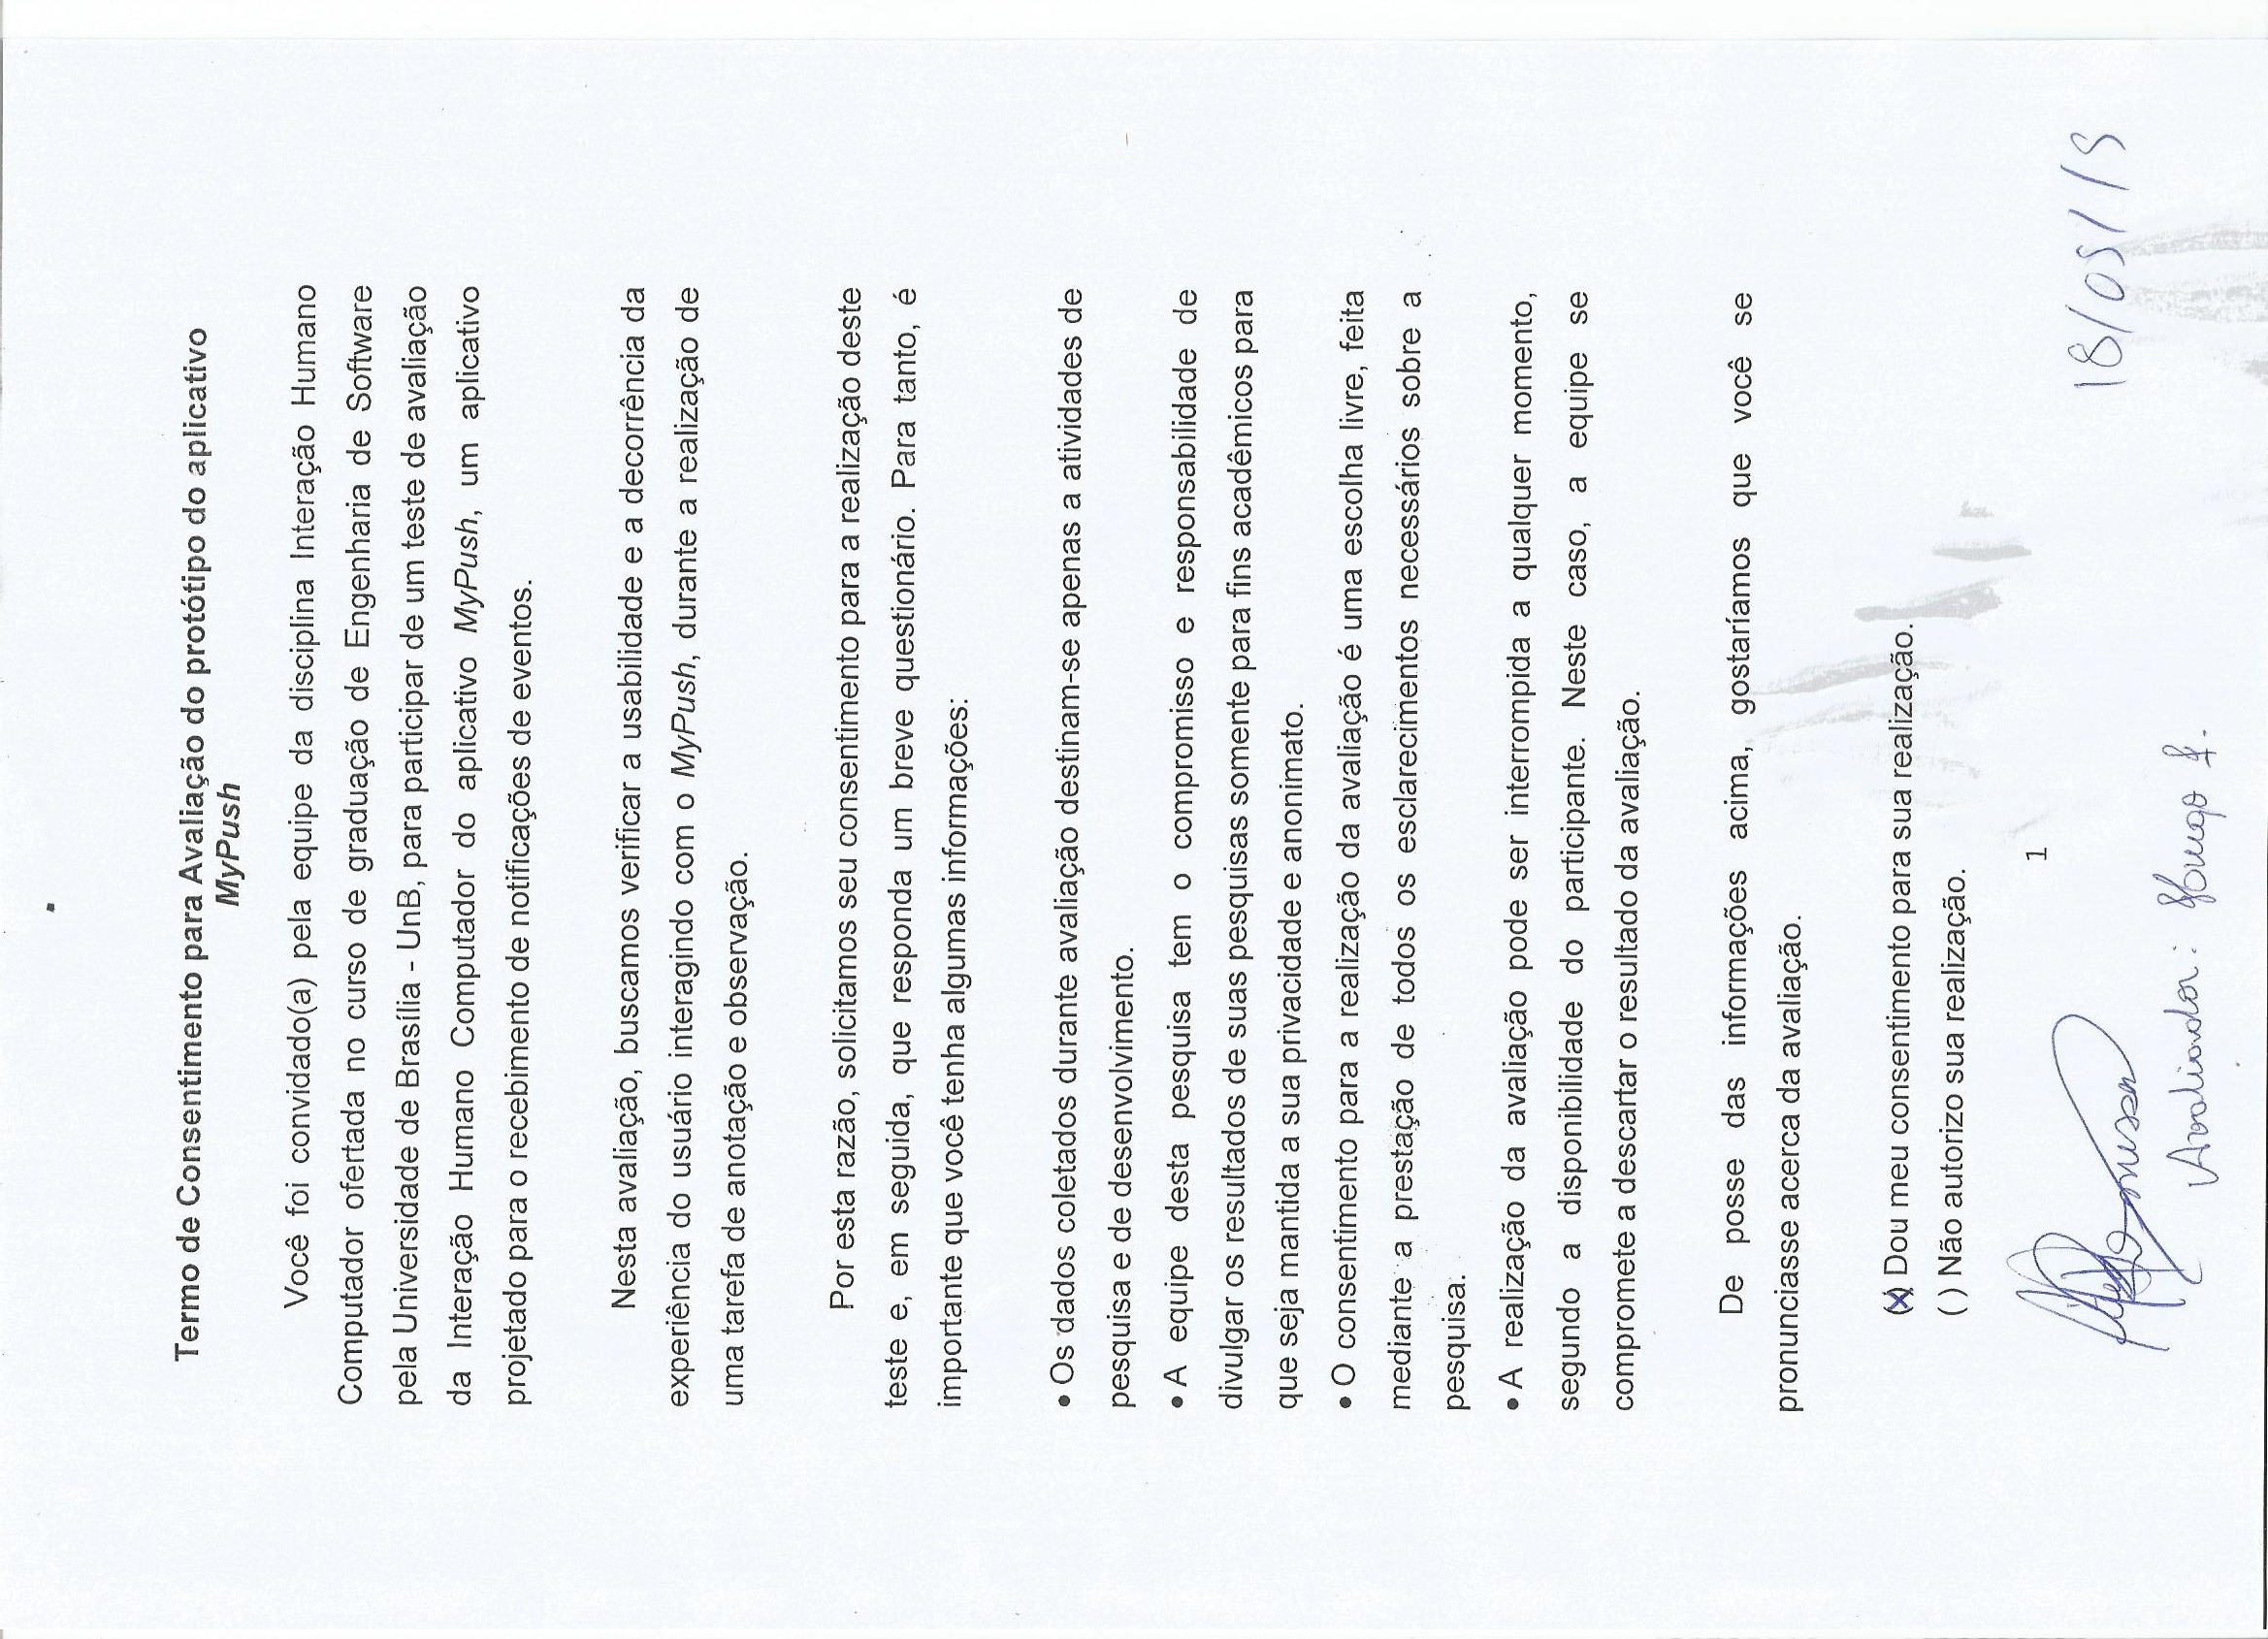
\includegraphics[scale=0.55, angle=-90]{editaveis/figuras/diego}
      \caption{Termo de consentimento assinado por um dos usuários que participaram da avaliação.}
      \label{termo_consentimento_1}
    \end{figure}
   
   \section*{Usuário 2}
    \begin{figure}[!htbp]
      \centering
      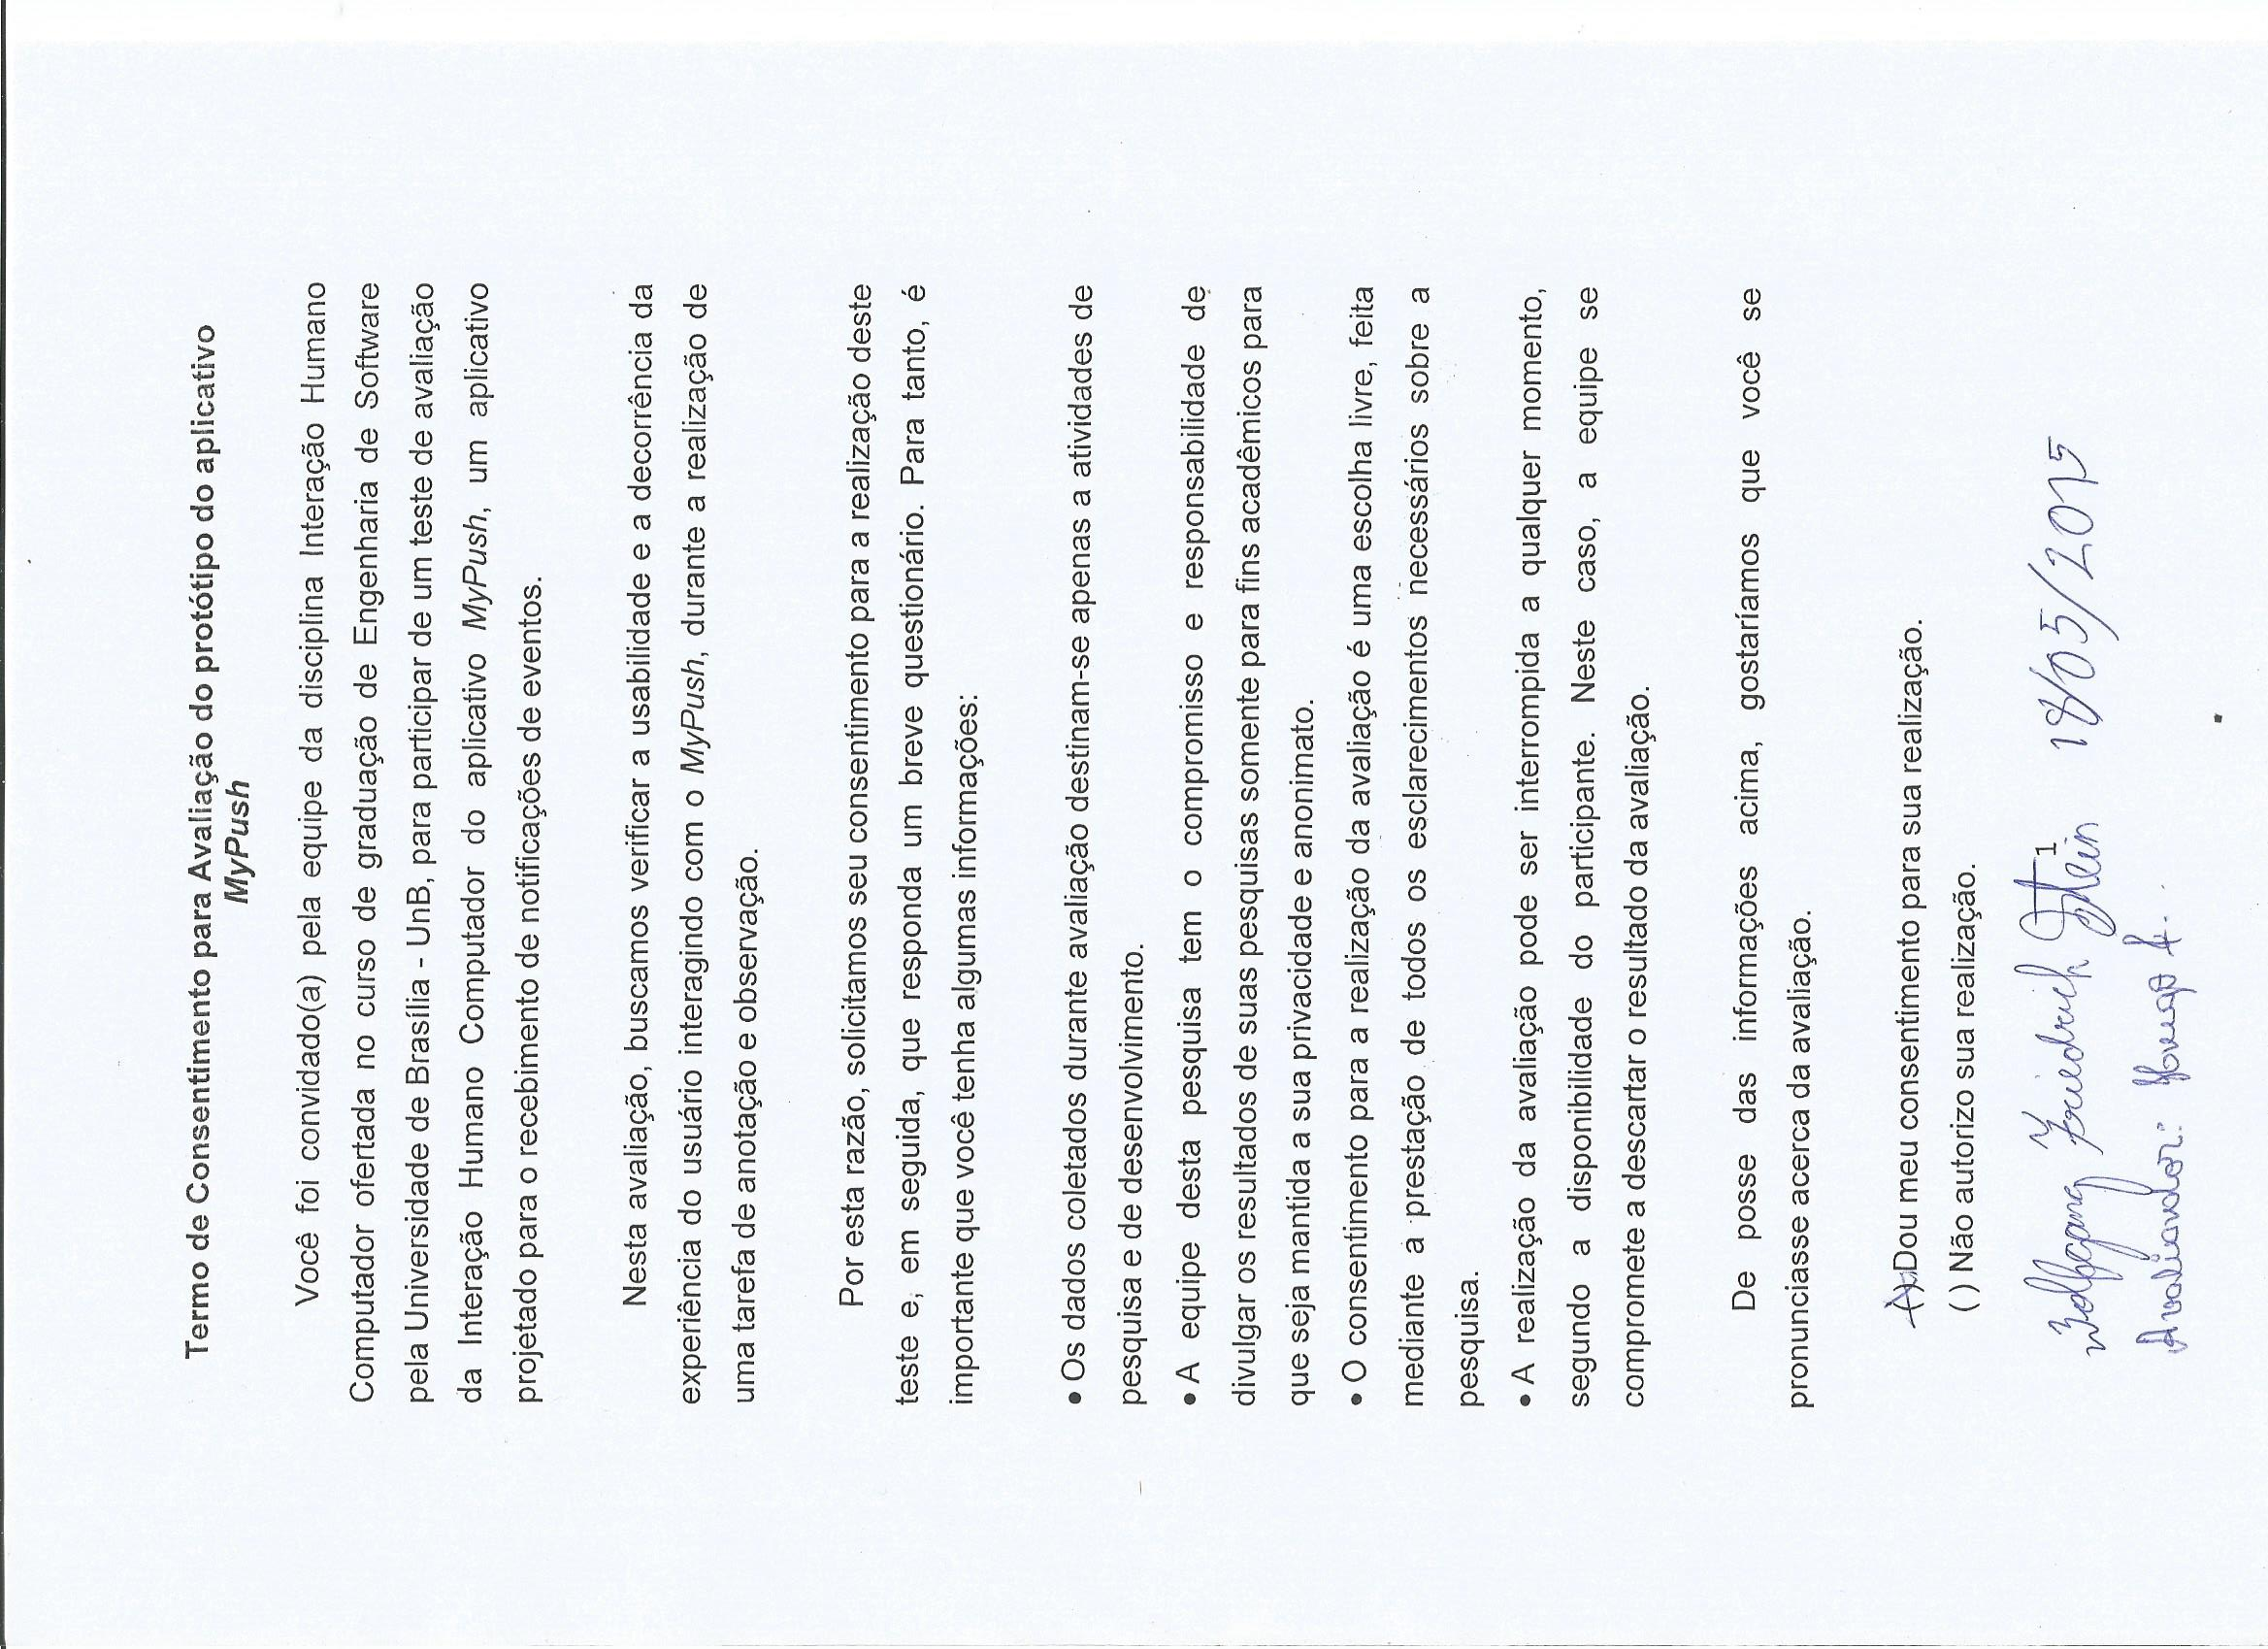
\includegraphics[scale=0.6, angle=-90]{editaveis/figuras/wolfgang}
      \caption{Termo de consentimento assinado por um dos usuários que participaram da avaliação.}
      \label{termo_consentimento_1}
    \end{figure}
    
       \section*{Usuário 3}
    \begin{figure}[!htbp]
      \centering
      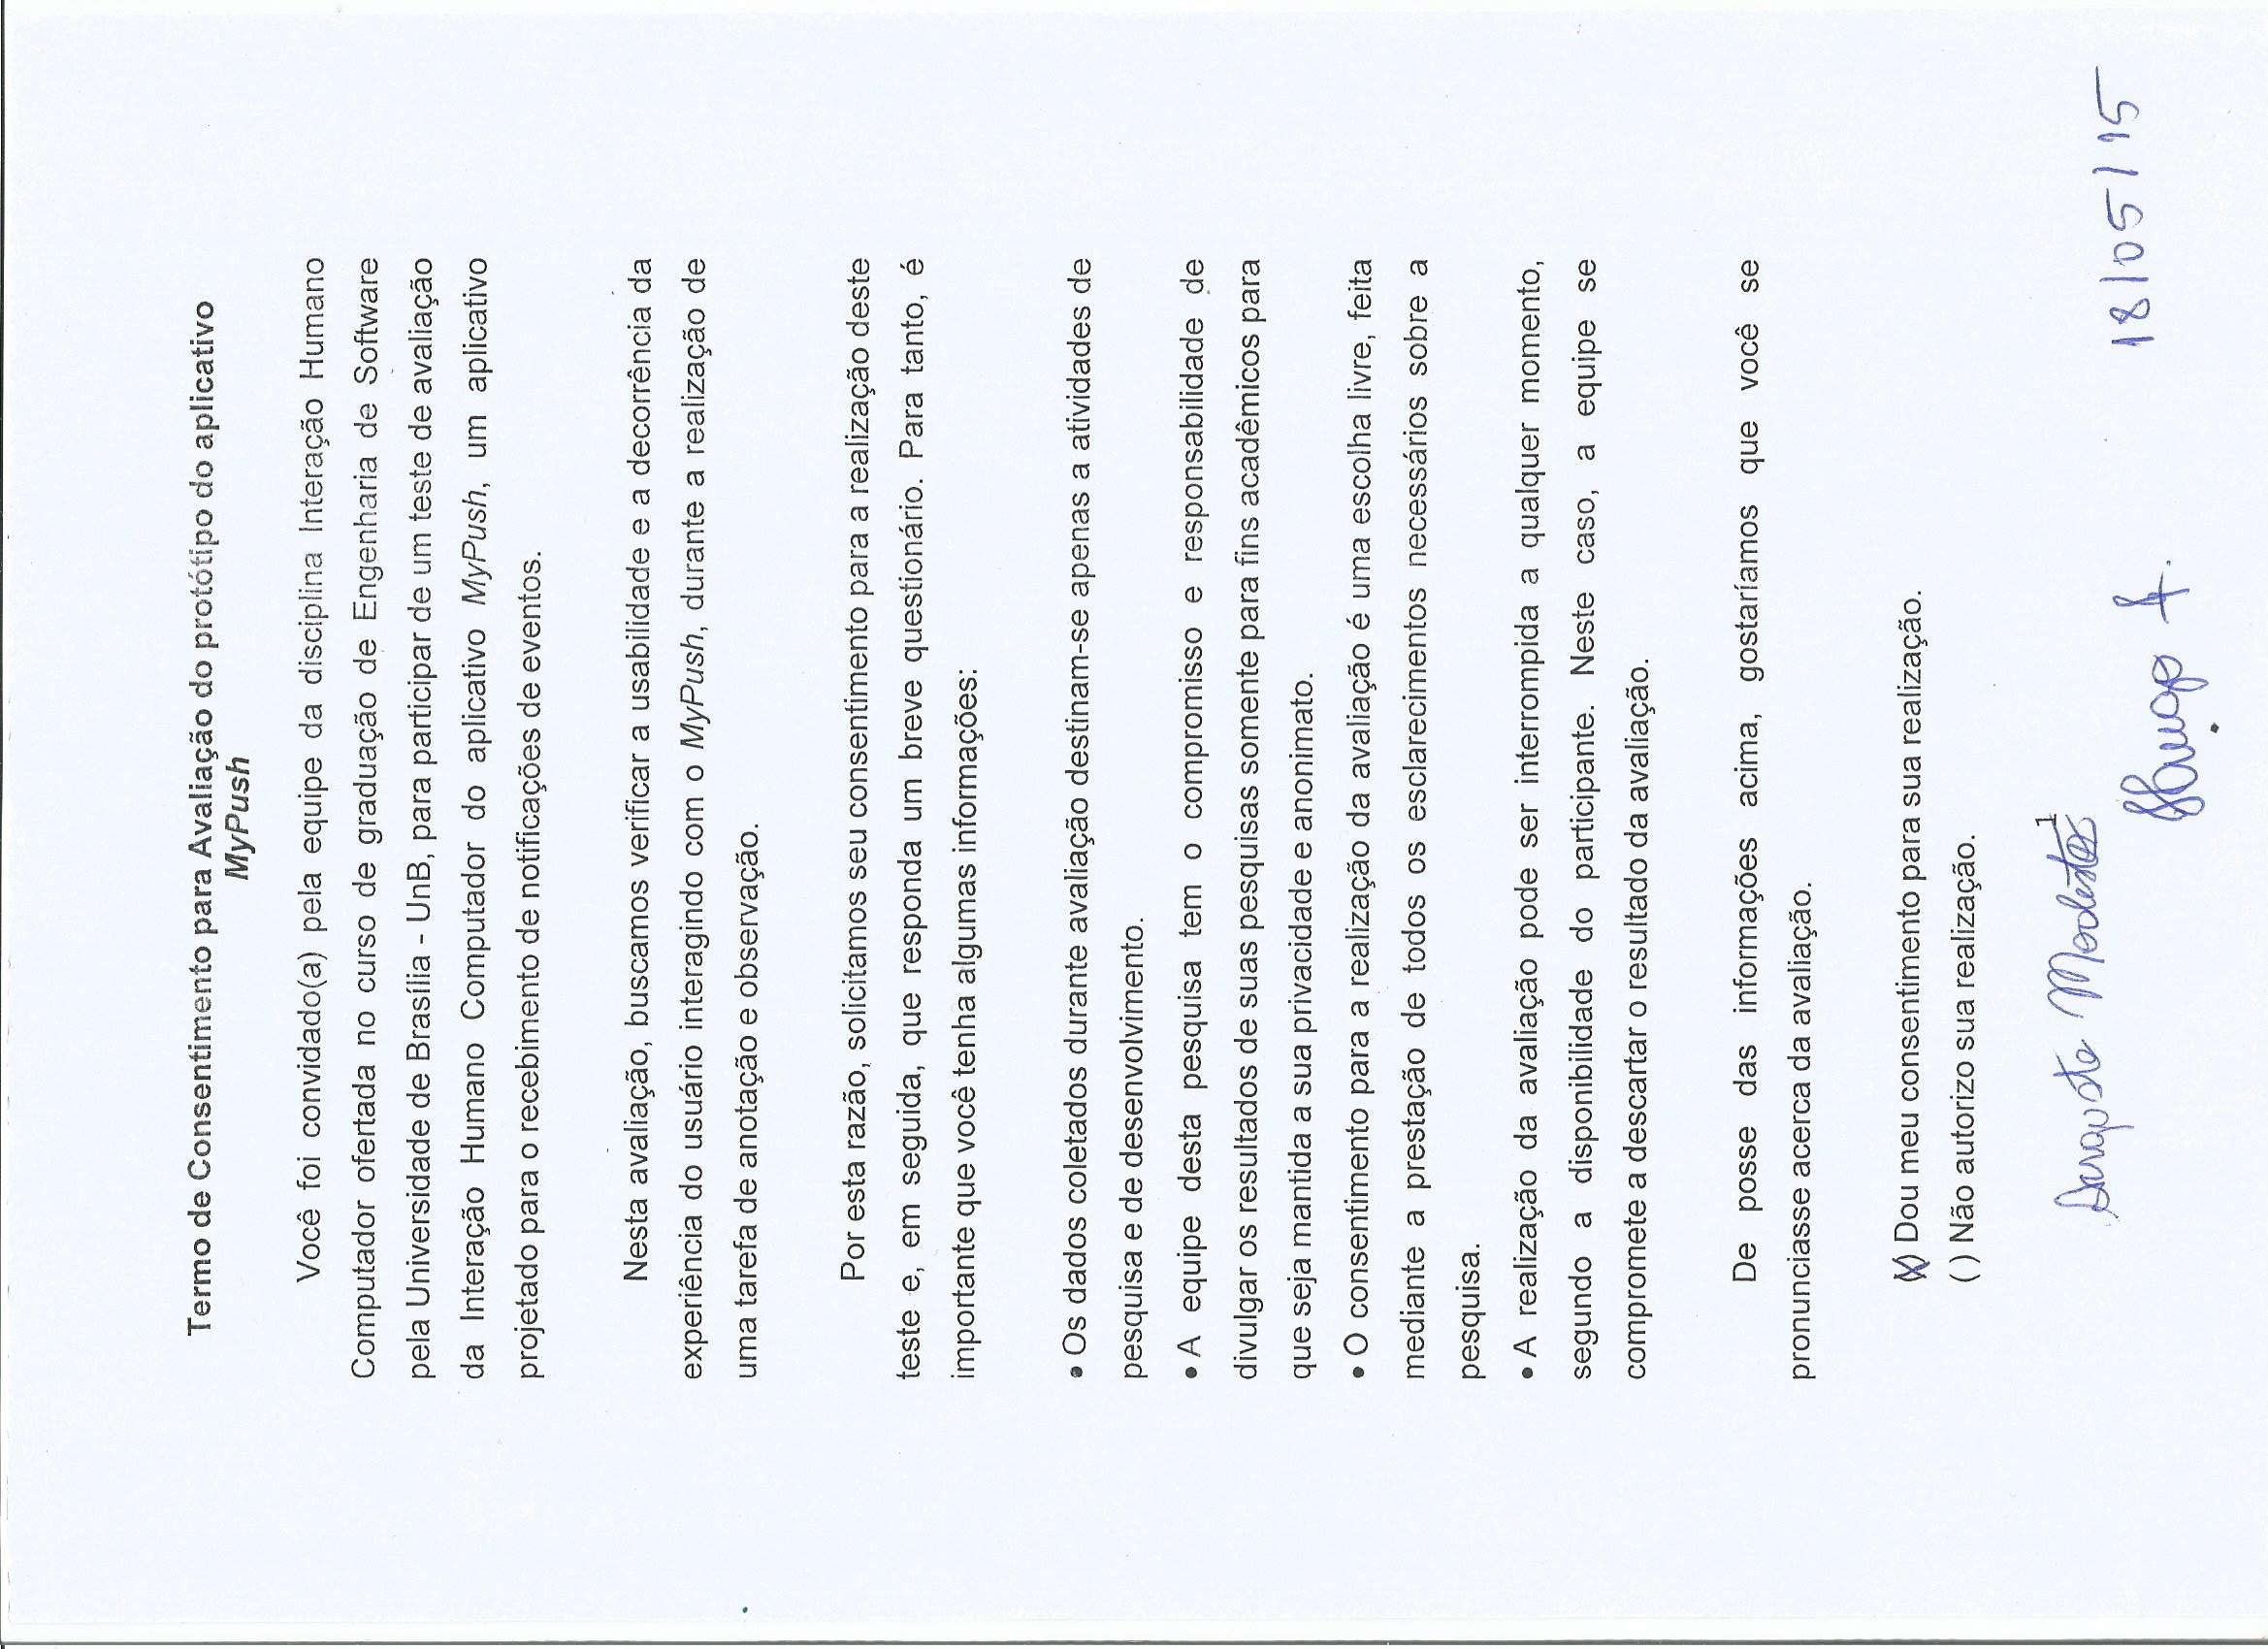
\includegraphics[scale=0.6, angle=-90]{editaveis/figuras/modesto}
      \caption{Termo de consentimento assinado por um dos usuários que participaram da avaliação.}
      \label{termo_consentimento_1}
    \end{figure}
    
       \section*{Usuário 4}
    \begin{figure}[!htbp]
      \centering
      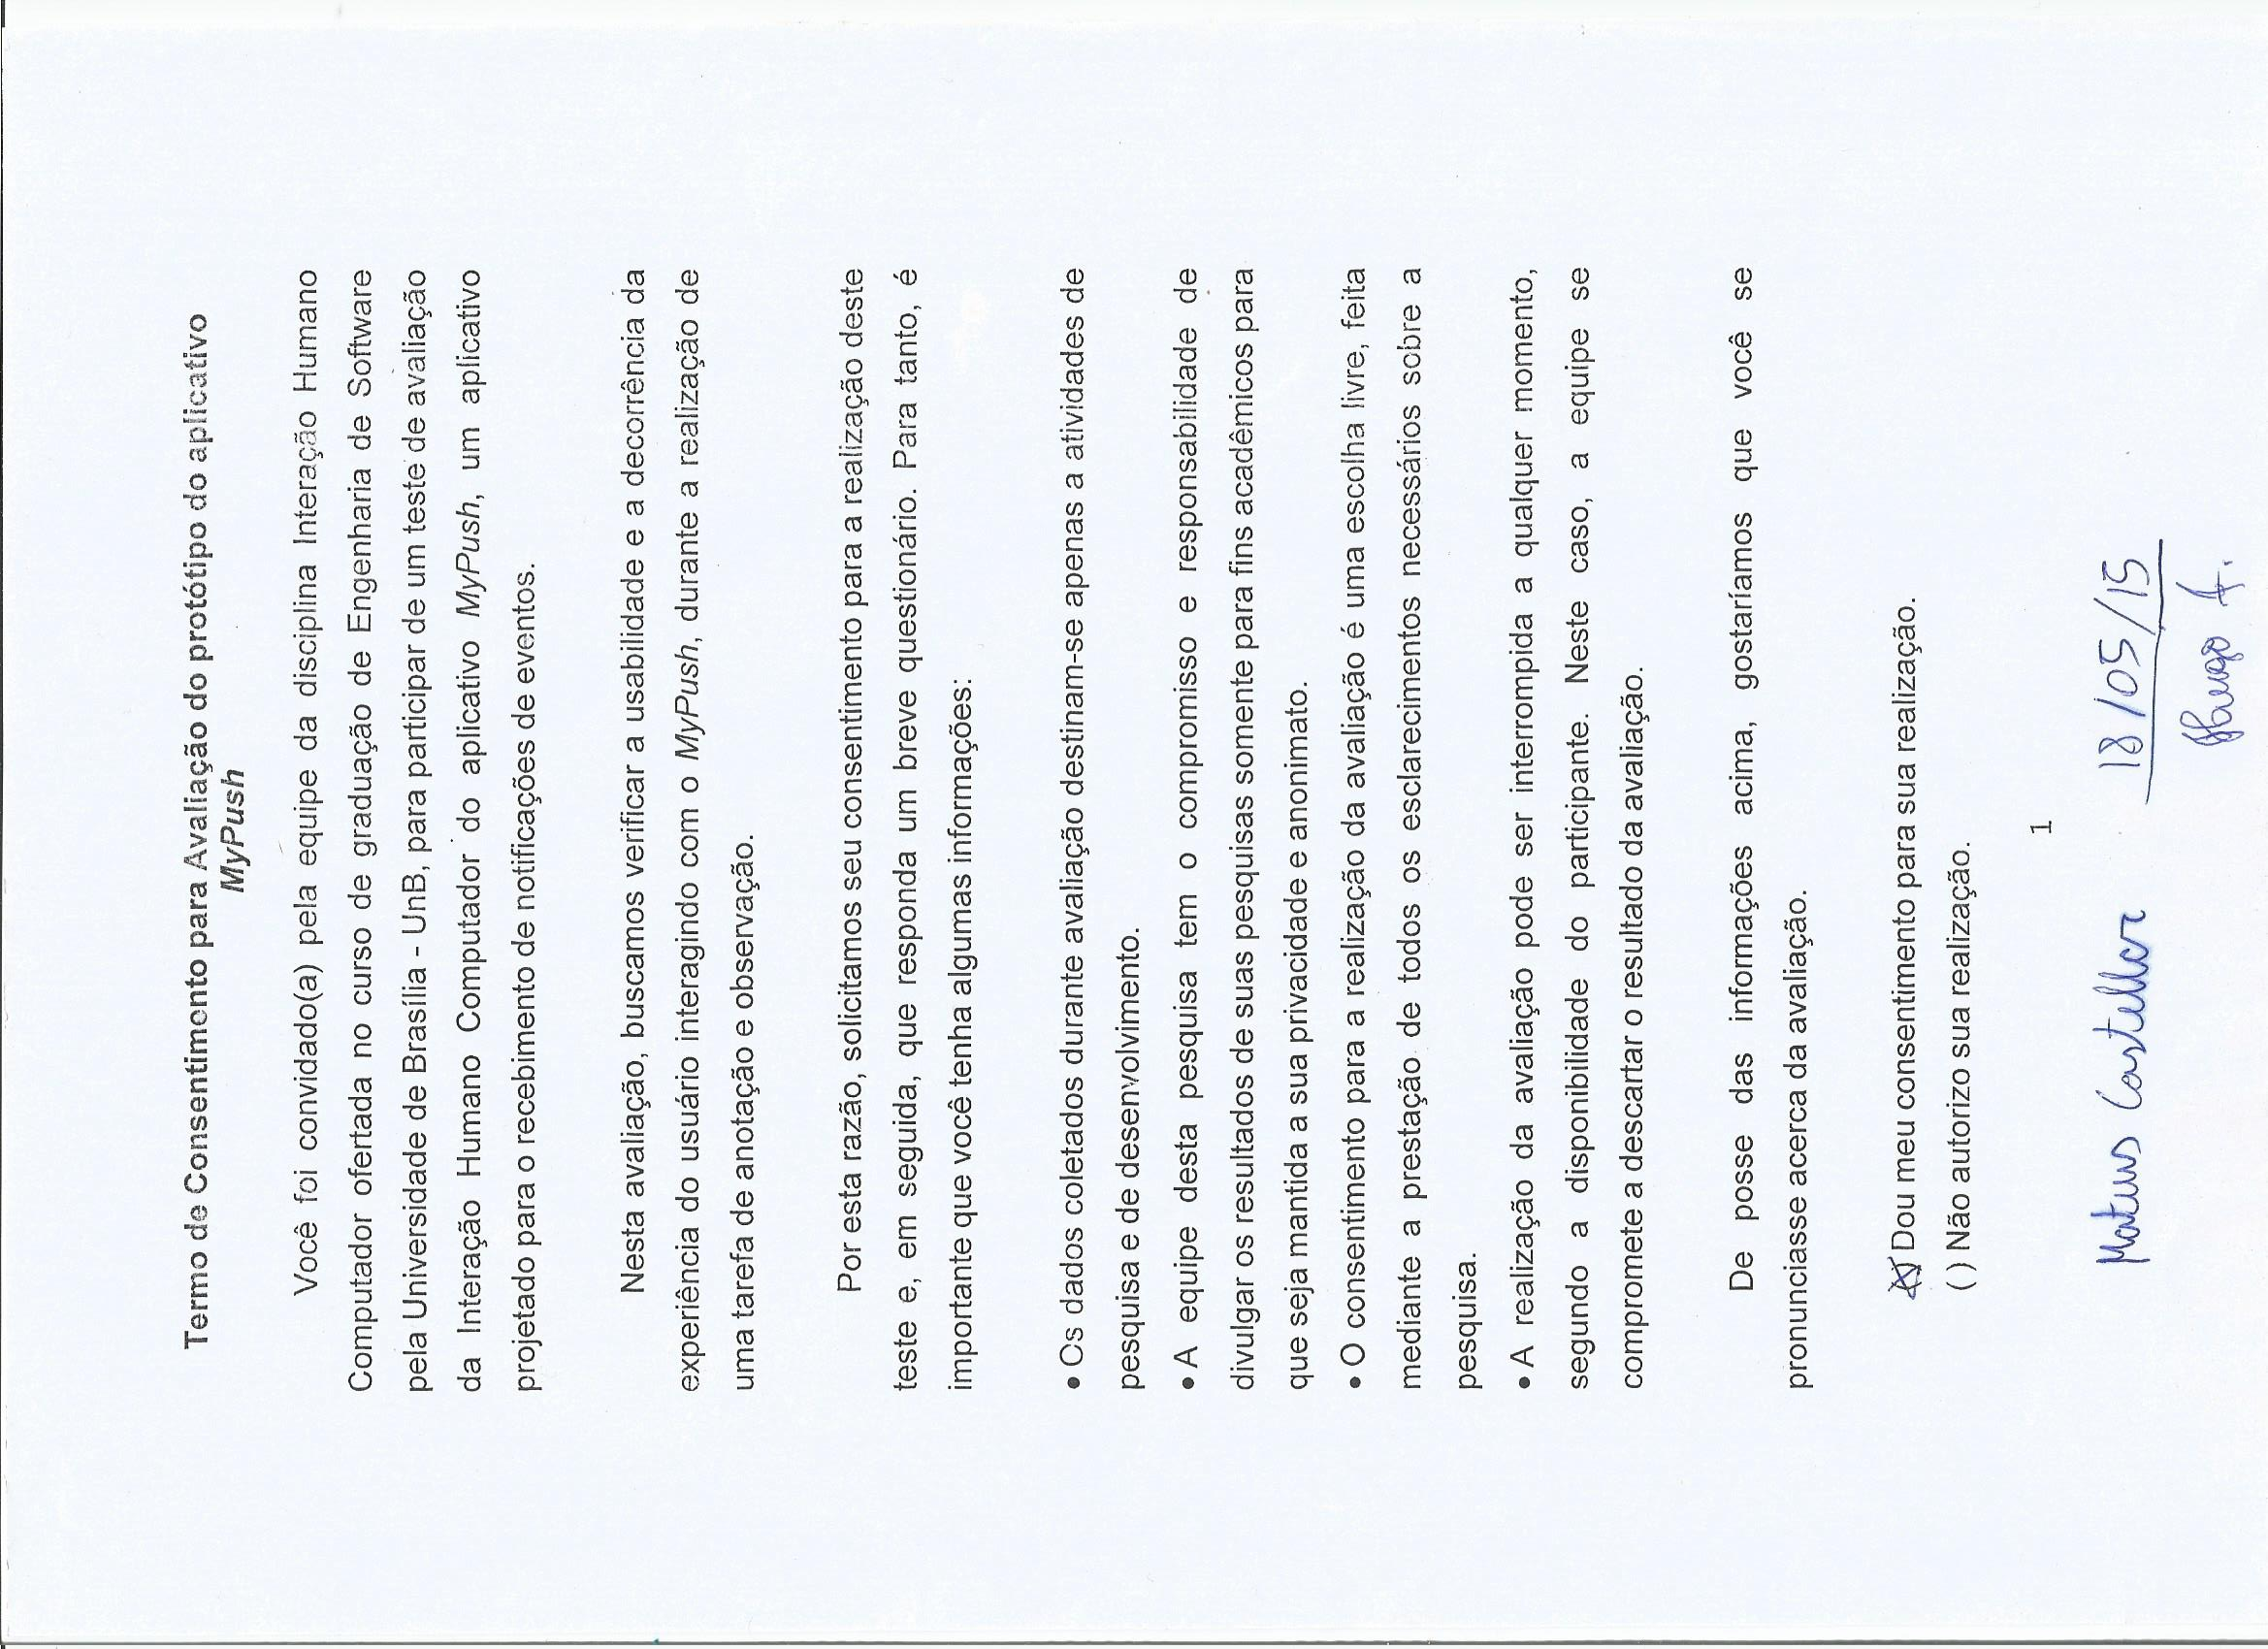
\includegraphics[scale=0.6, angle=-90]{editaveis/figuras/castellar}
      \caption{Termo de consentimento assinado por um dos usuários que participaram da avaliação.}
      \label{termo_consentimento_1}
    \end{figure}
    
       \section*{Usuário 5}
    \begin{figure}[!htbp]
      \centering
      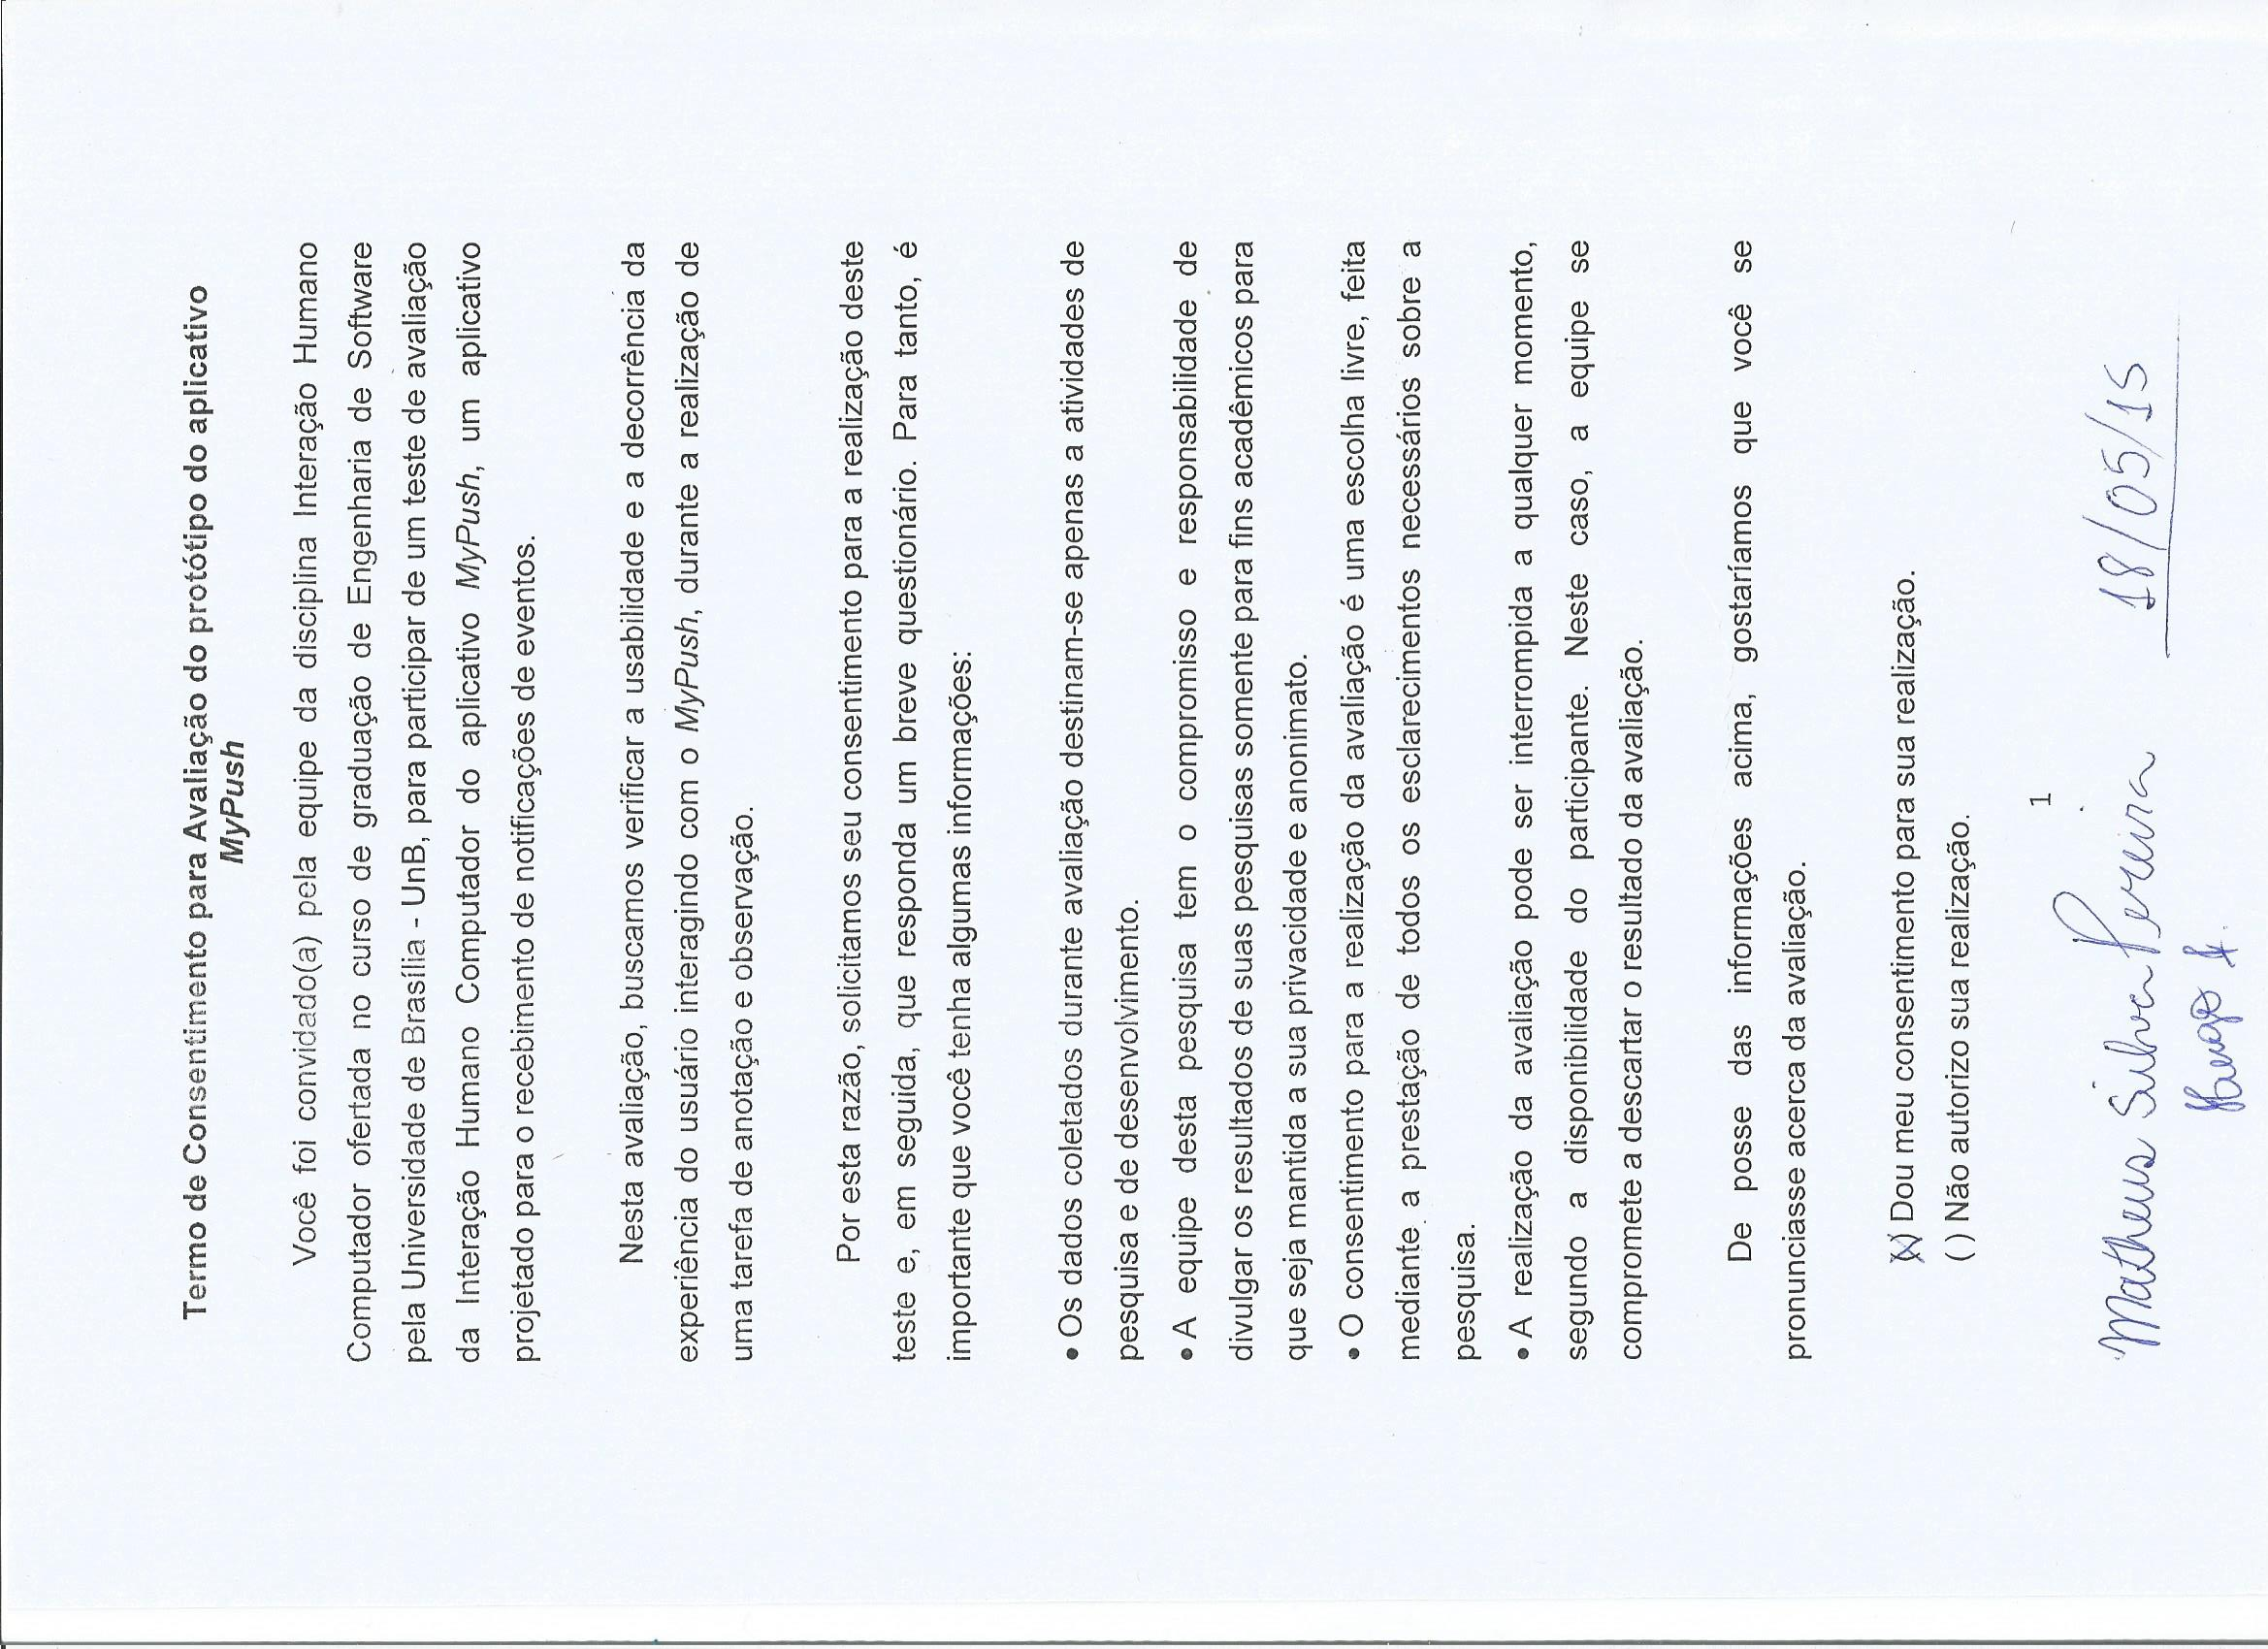
\includegraphics[scale=0.6, angle=-90]{editaveis/figuras/silva}
      \caption{Termo de consentimento assinado por um dos usuários que participaram da avaliação.}
      \label{termo_consentimento_1}
    \end{figure}
    
      \section*{Usuário 6}
    \begin{figure}[!htbp]
      \centering
      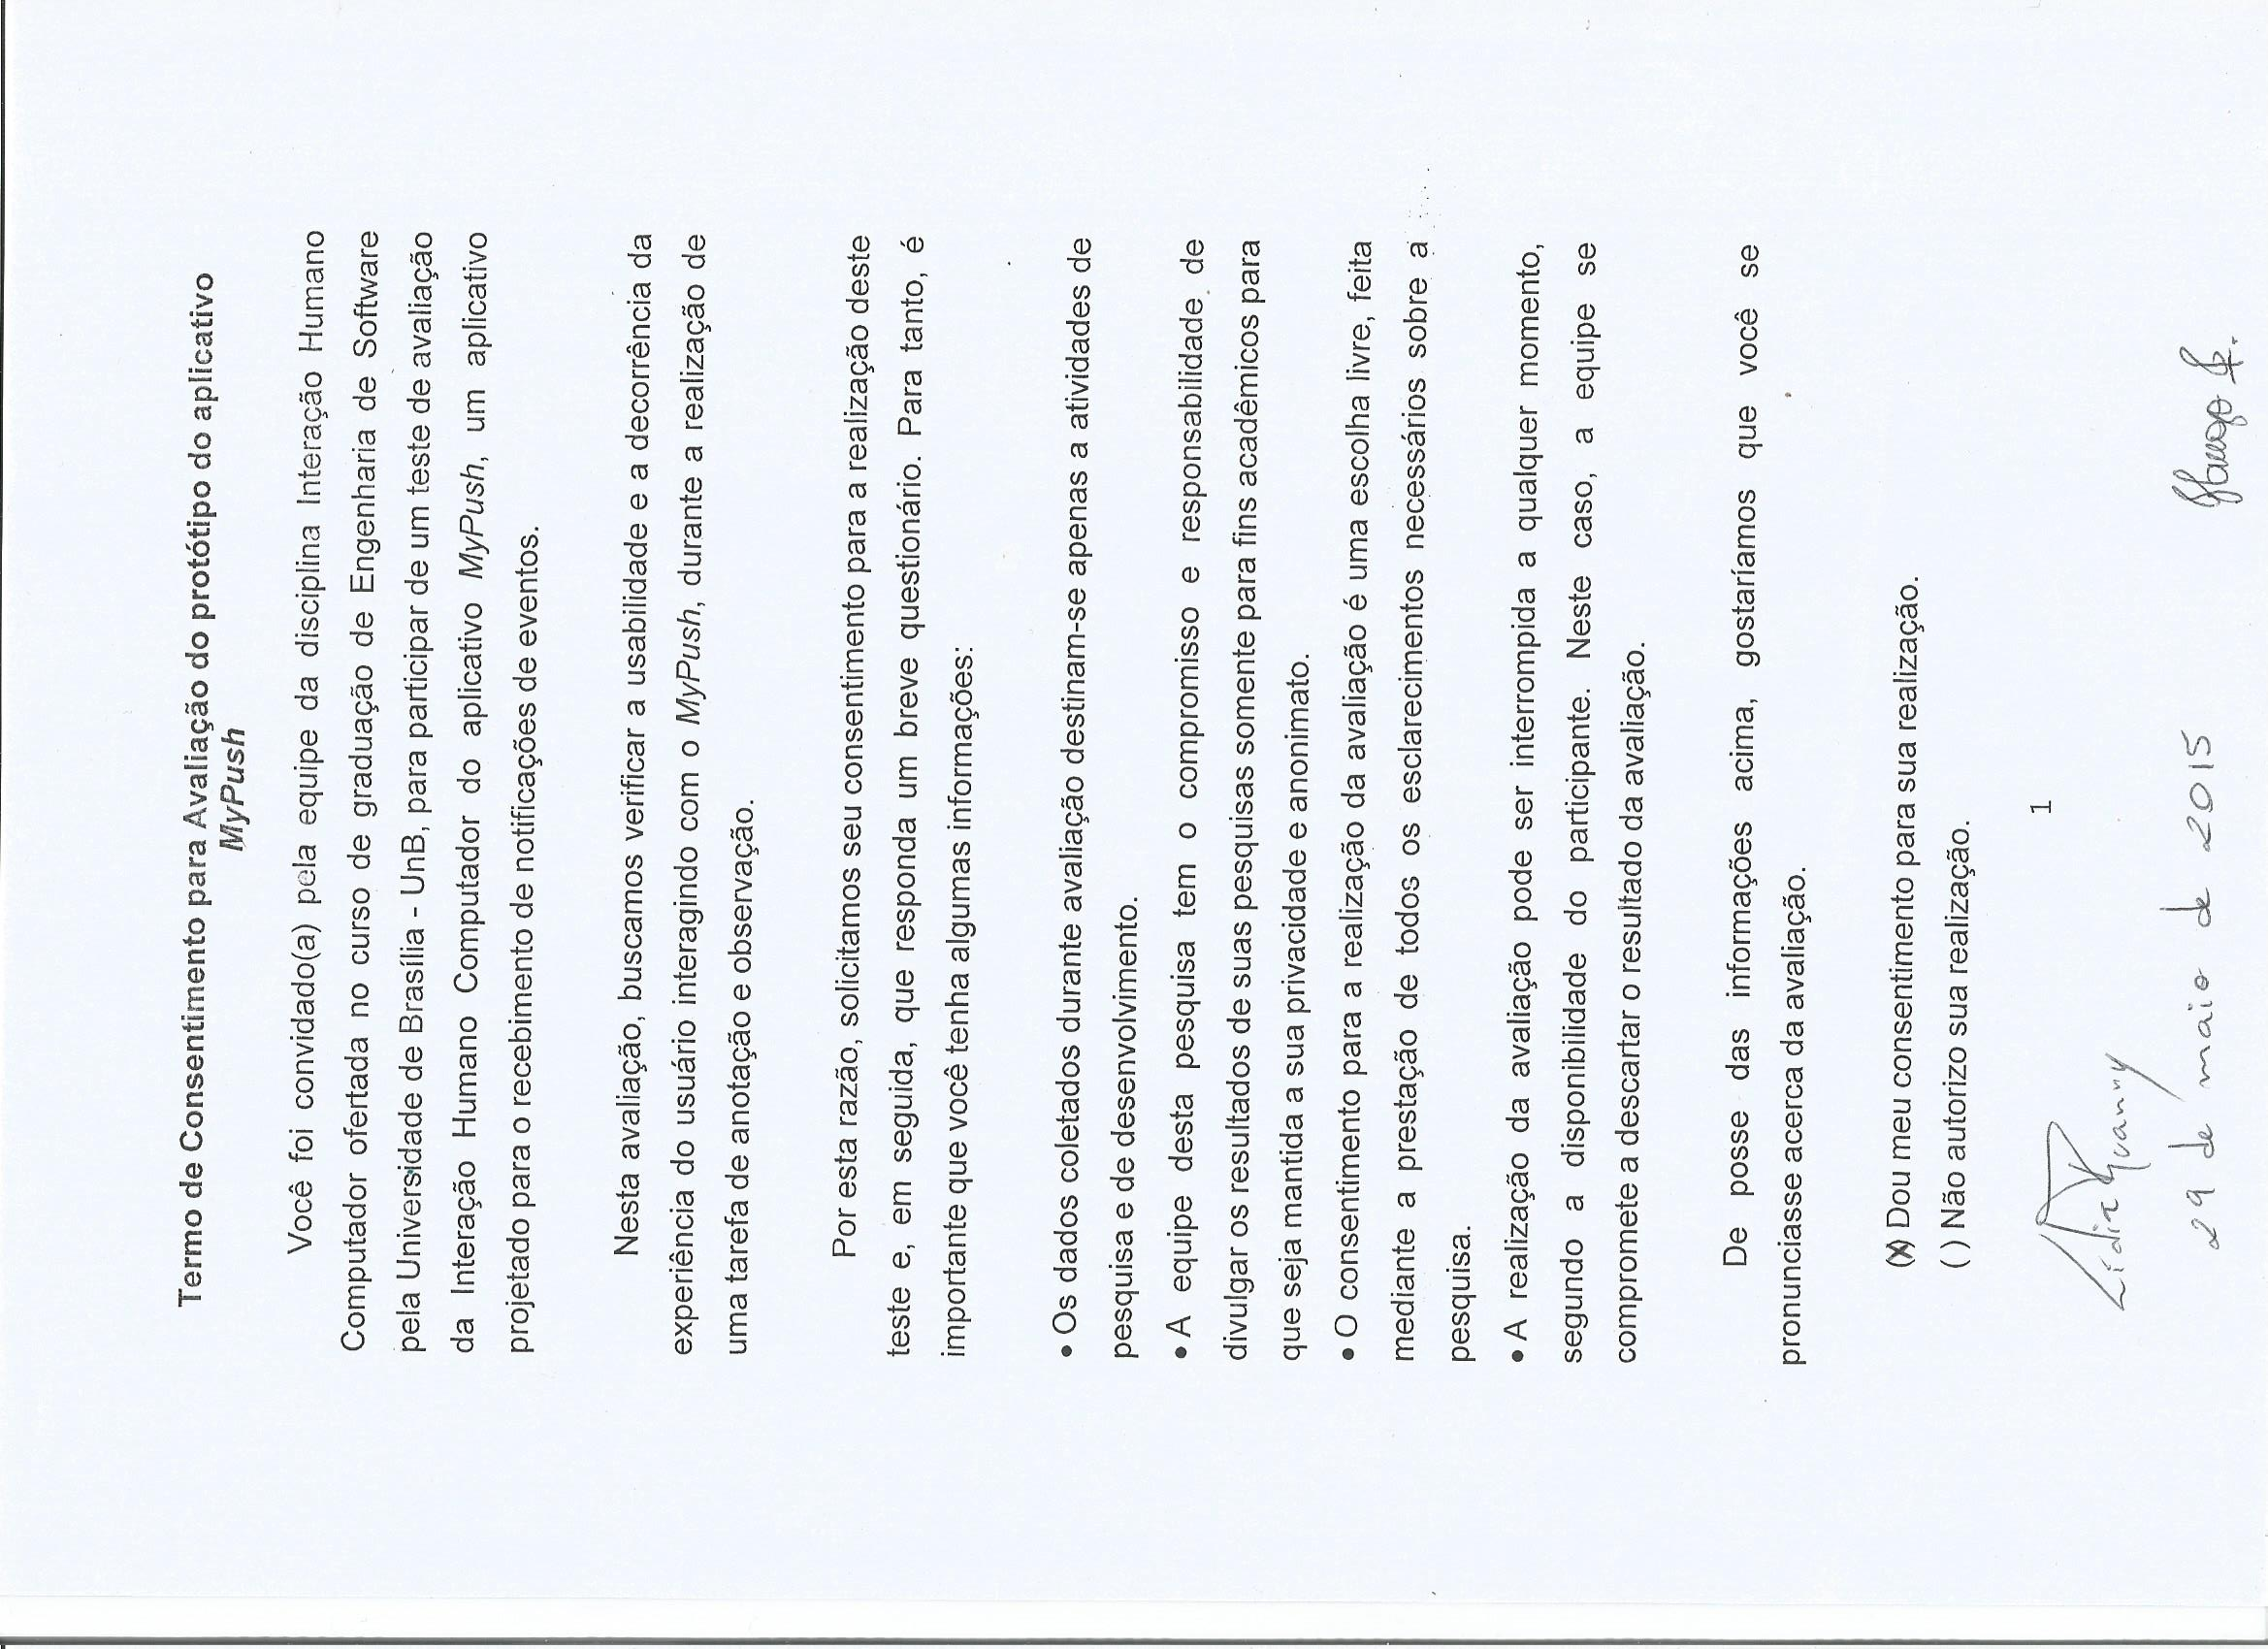
\includegraphics[scale=0.6, angle=-90]{editaveis/figuras/lidia}
      \caption{Termo de consentimento assinado por um dos usuários que participaram da avaliação.}
      \label{termo_consentimento_1}
    \end{figure}
    
      \section*{Usuário 7}
    \begin{figure}[!htbp]
      \centering
      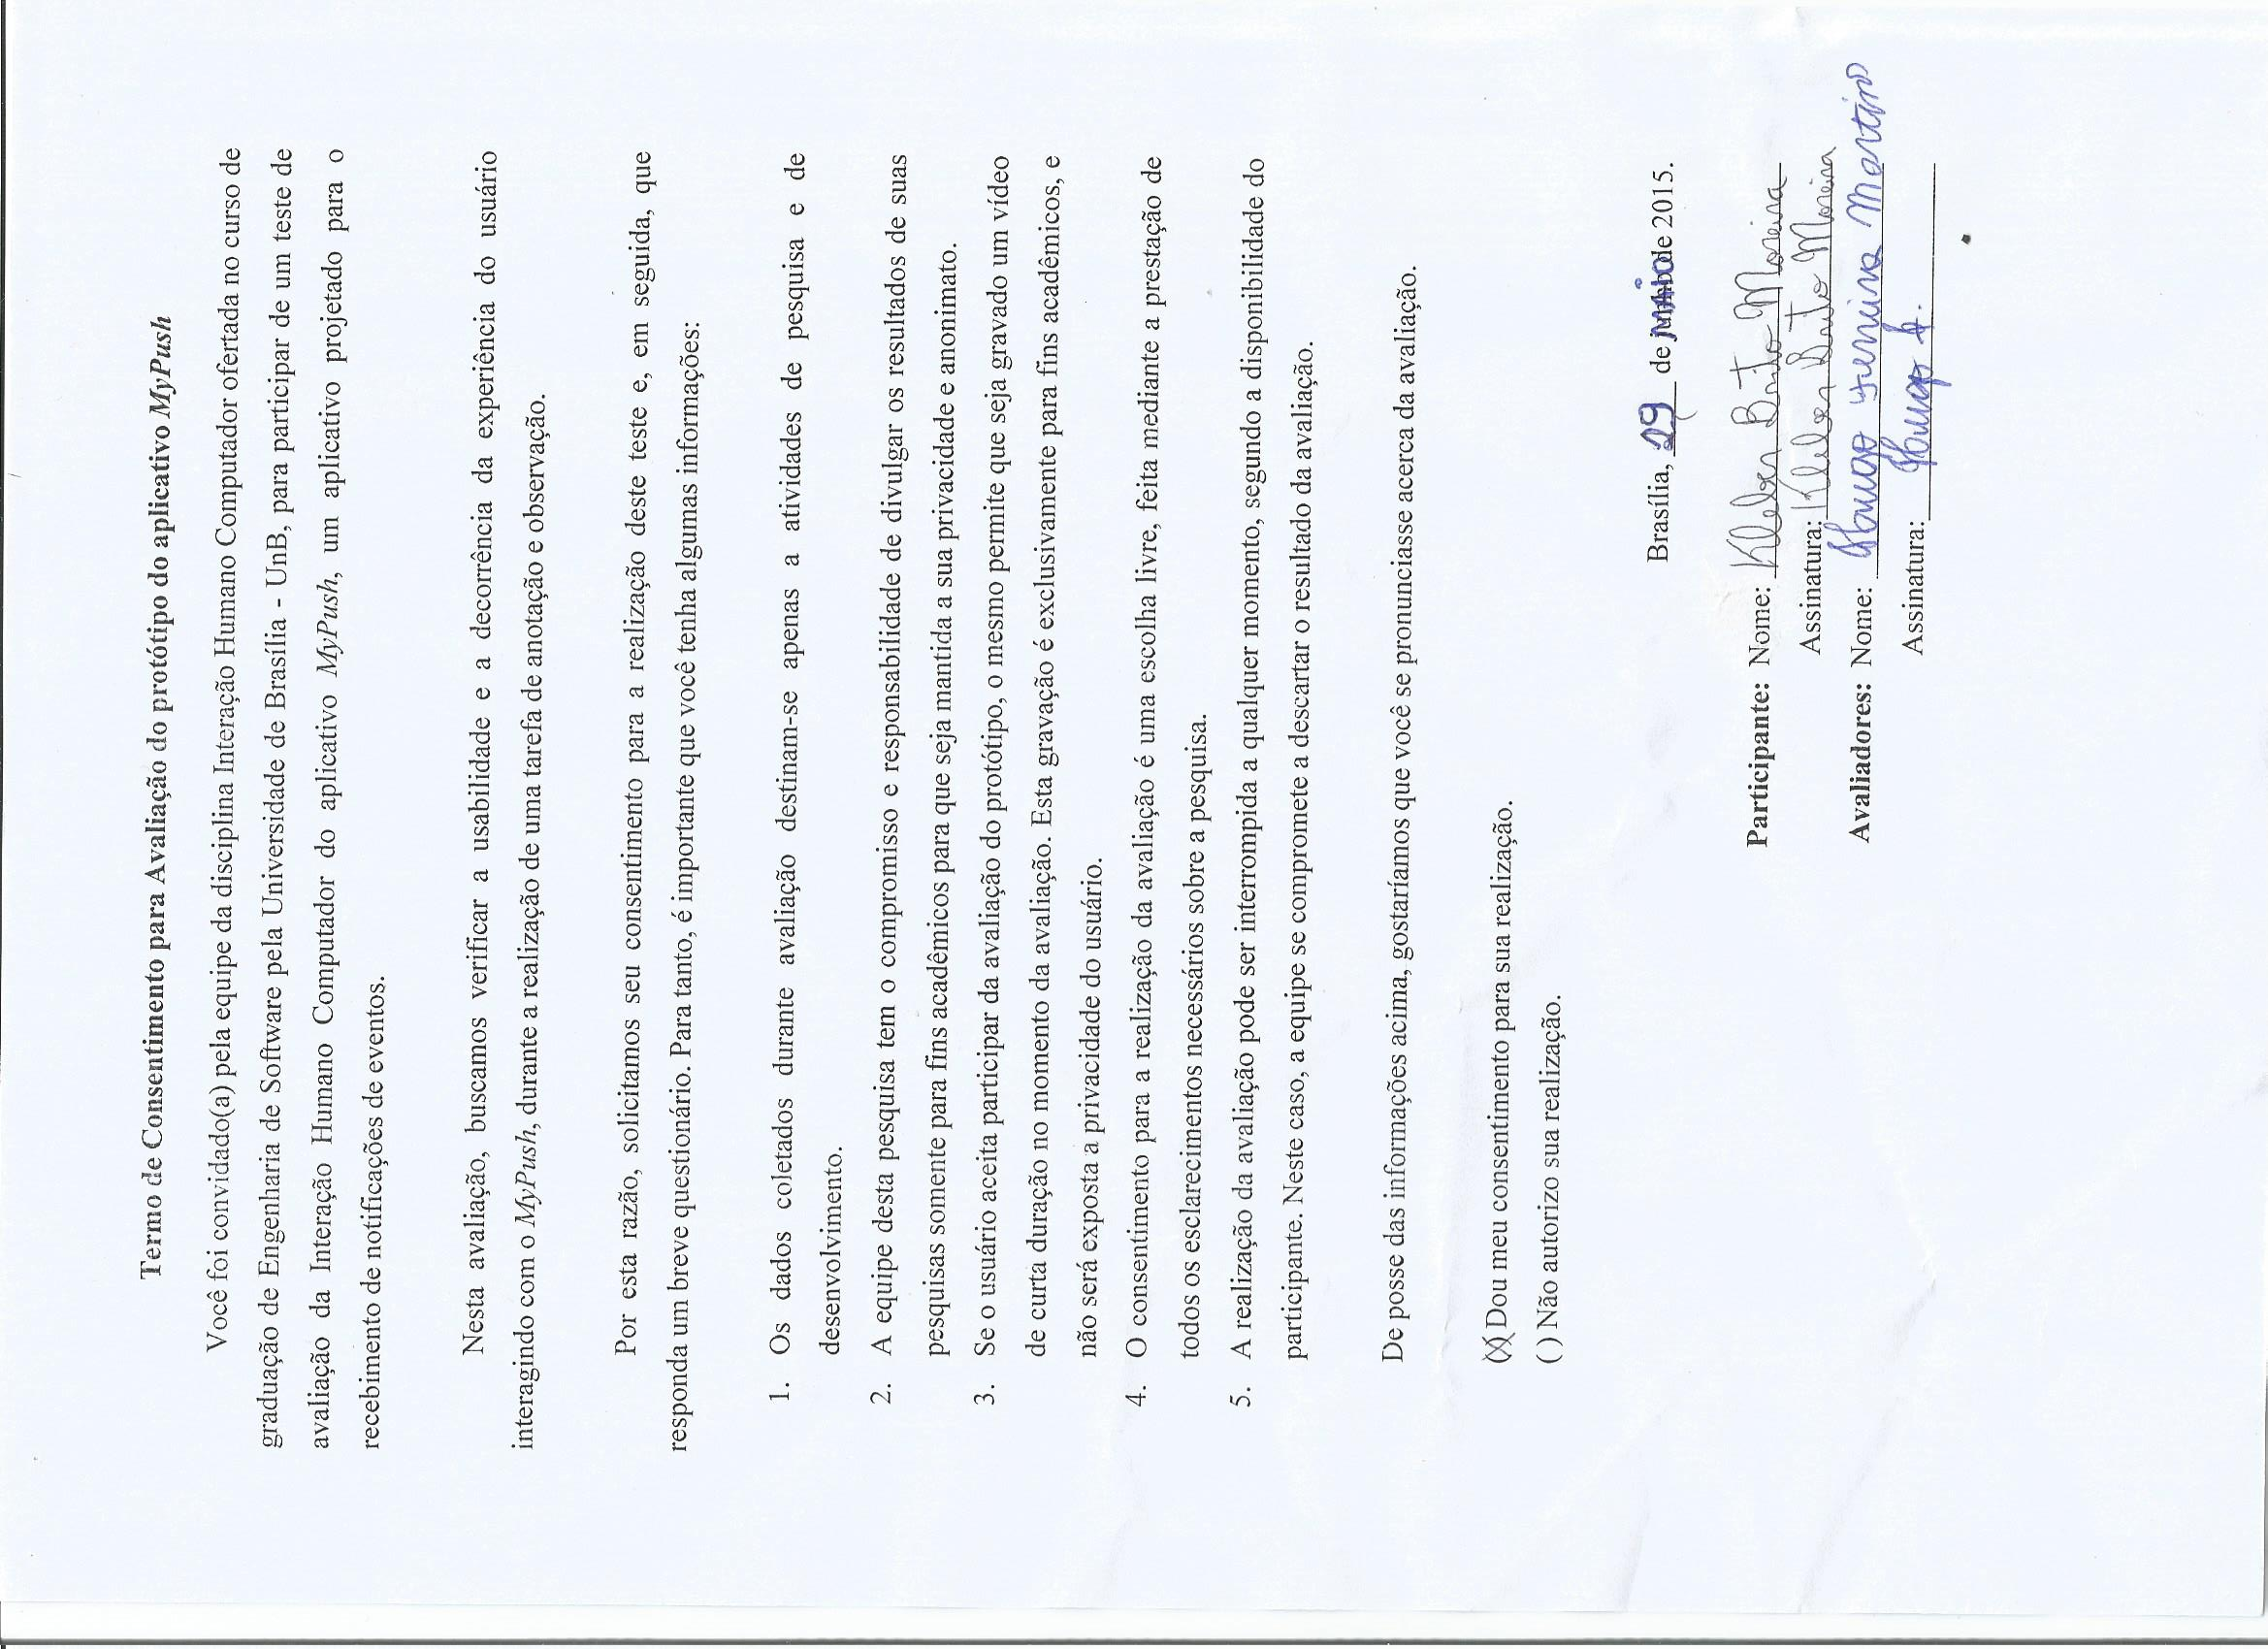
\includegraphics[scale=0.6, angle=-90]{editaveis/figuras/kleber}
      \caption{Termo de consentimento assinado por um dos usuários que participaram da avaliação.}
      \label{termo_consentimento_1}
    \end{figure}
    
      \section*{Usuário 8}
    \begin{figure}[!htbp]
      \centering
      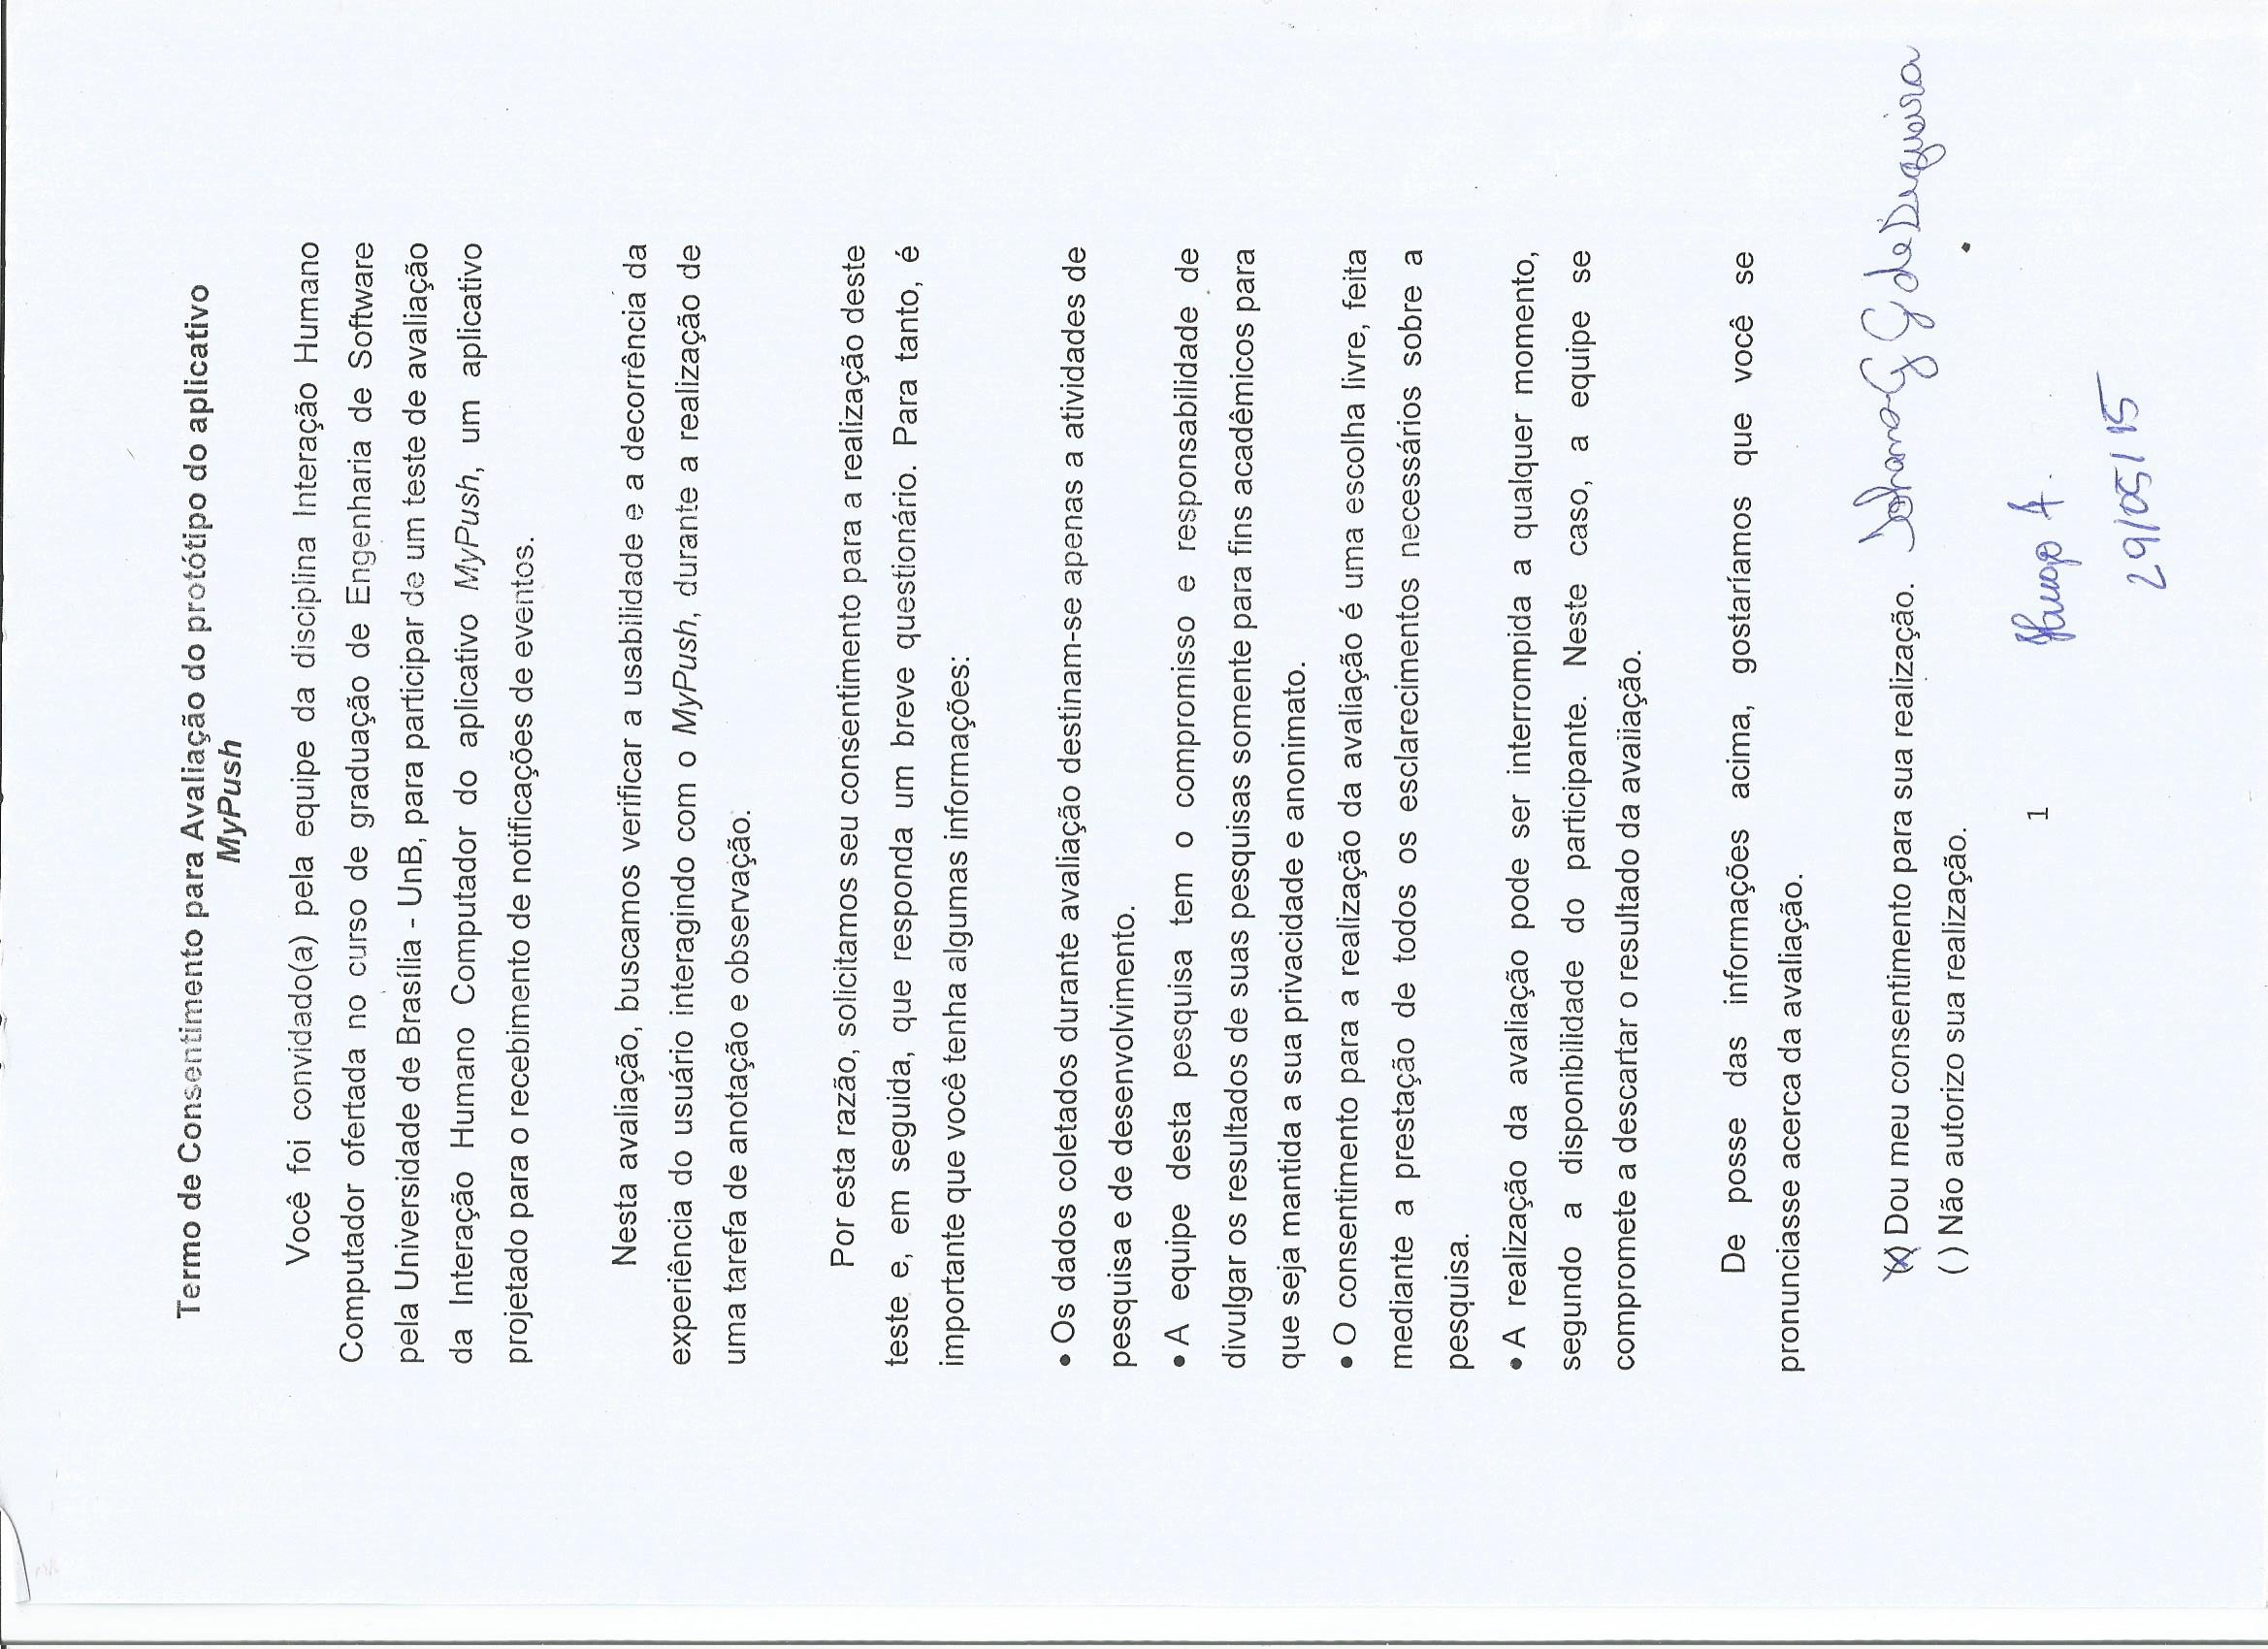
\includegraphics[scale=0.6, angle=-90]{editaveis/figuras/iohana}
      \caption{Termo de consentimento assinado por um dos usuários que participaram da avaliação.}
      \label{termo_consentimento_1}
    \end{figure}
    
      \section*{Usuário 9}
    \begin{figure}[!htbp]
      \centering
      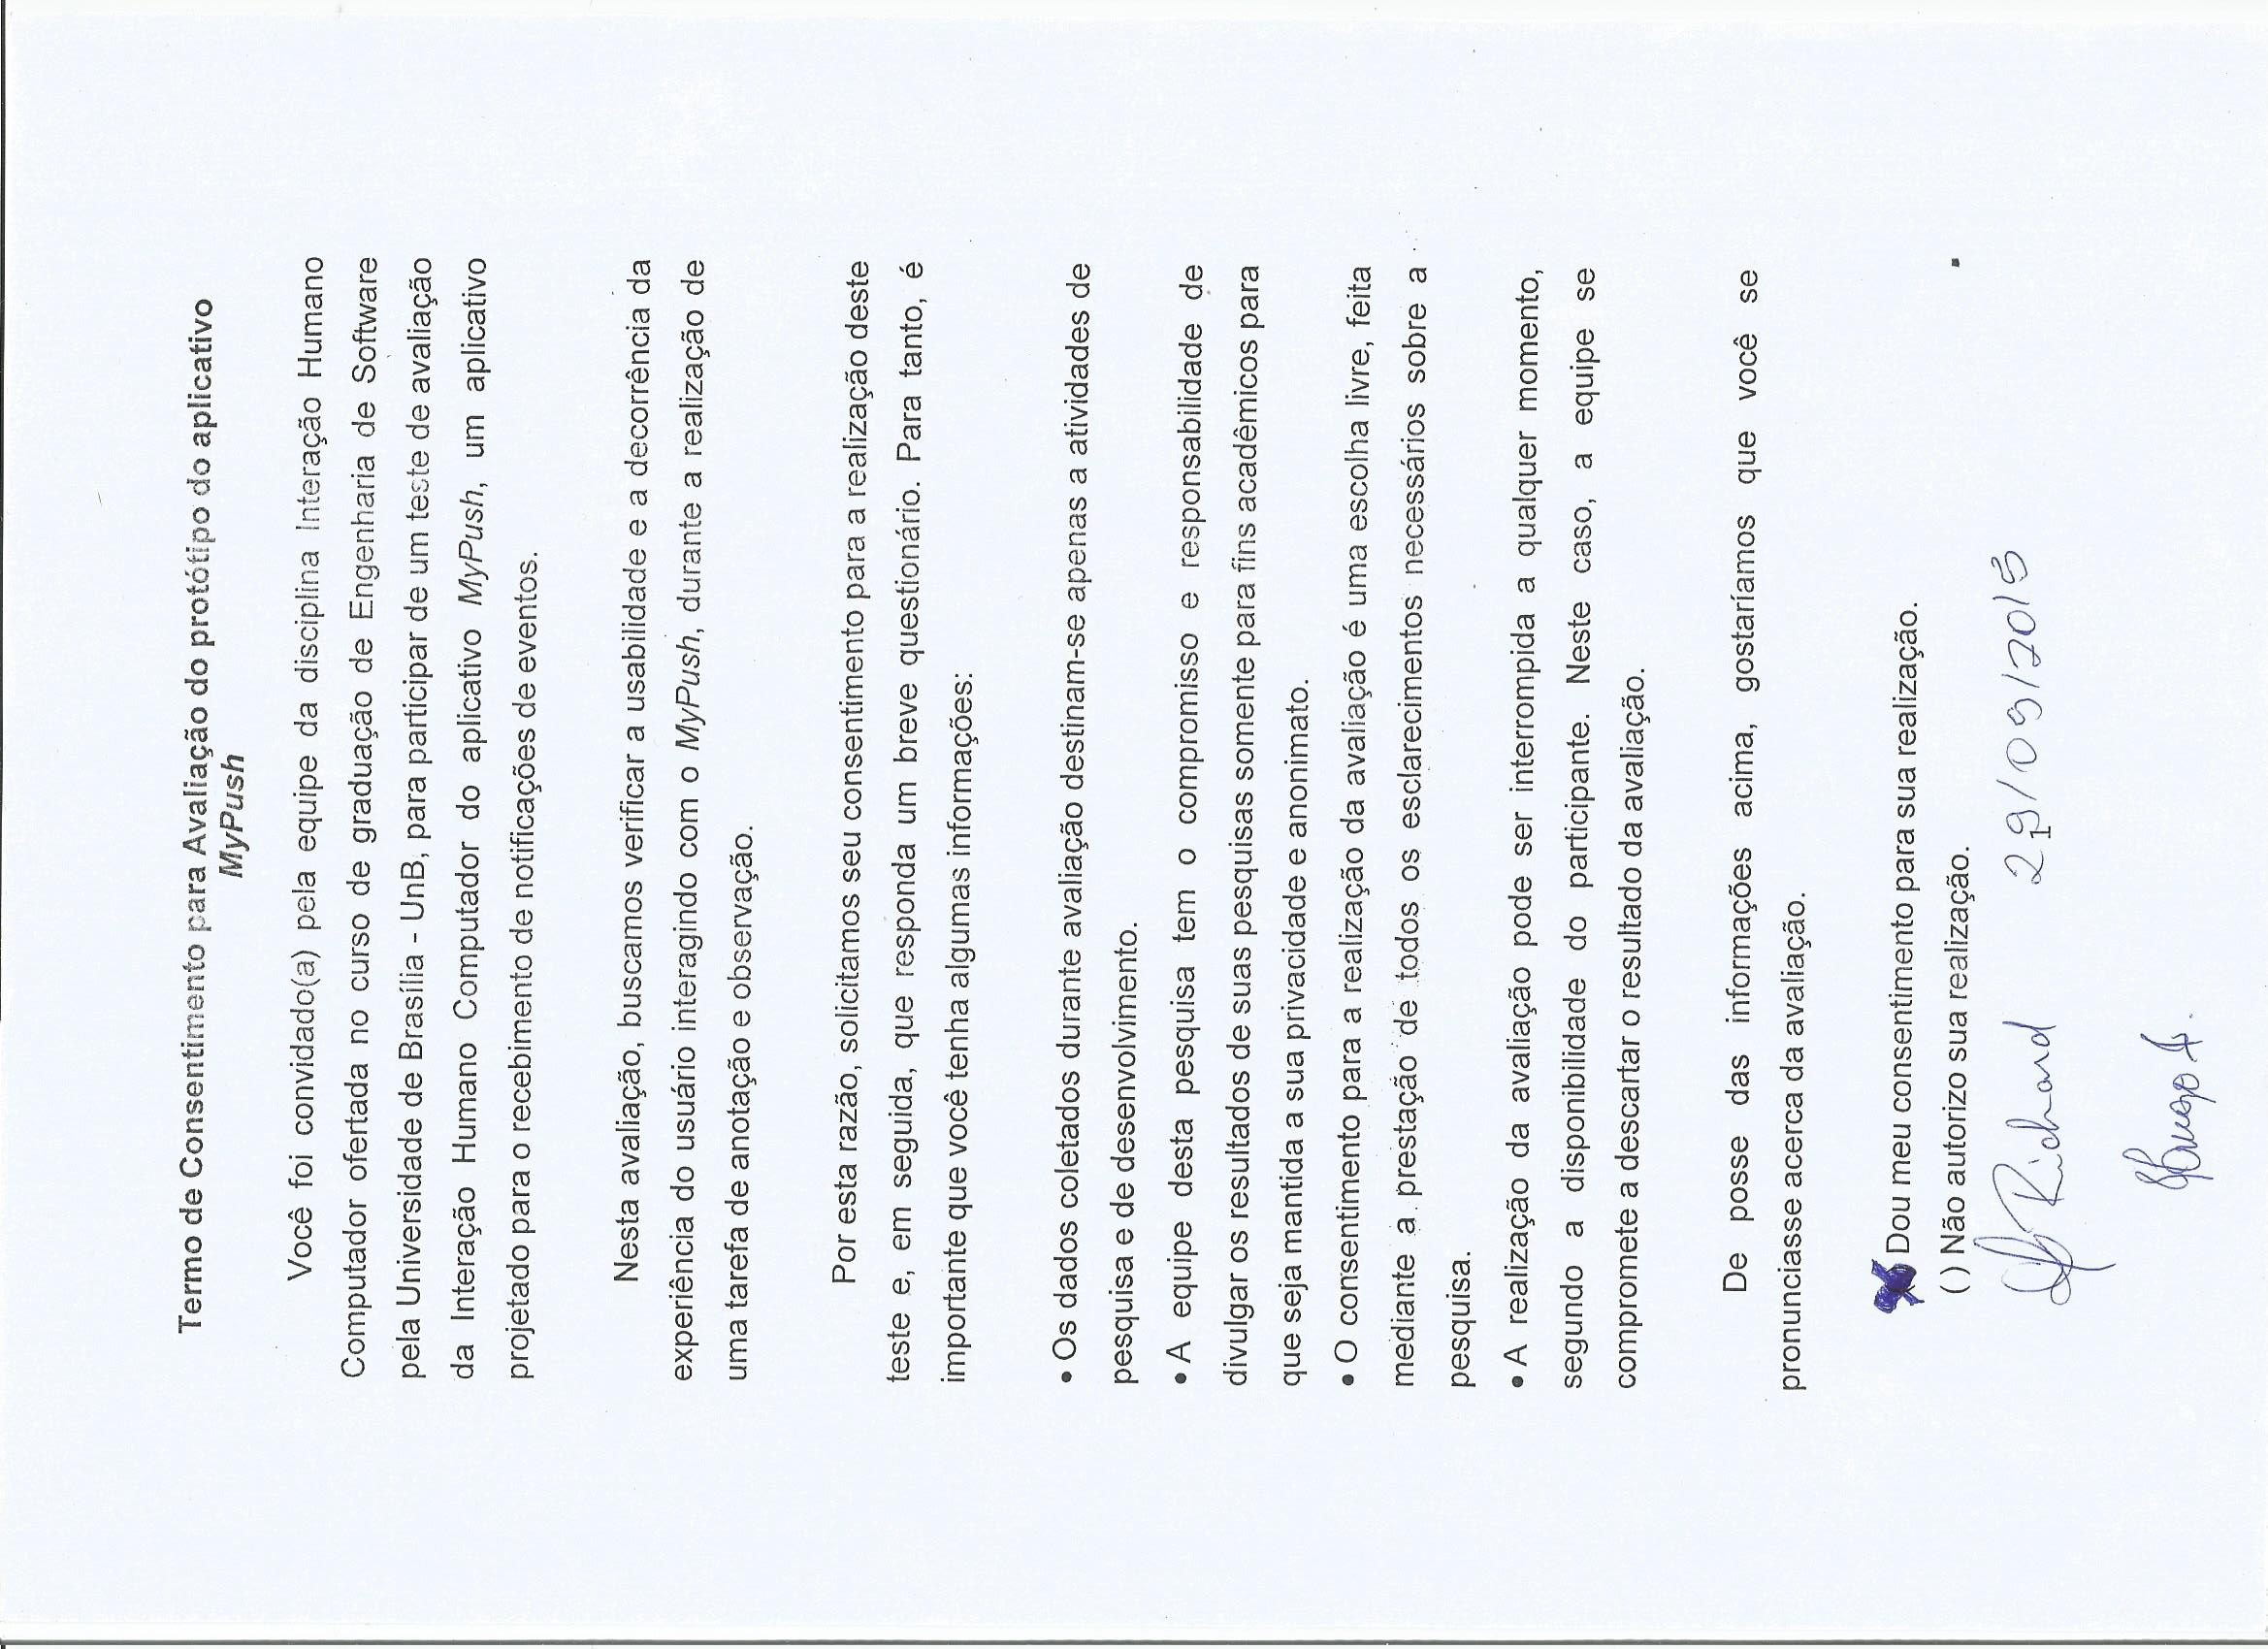
\includegraphics[scale=0.6, angle=-90]{editaveis/figuras/guilherme}
      \caption{Termo de consentimento assinado por um dos usuários que participaram da avaliação.}
      \label{termo_consentimento_1}
    \end{figure}
    
      \section*{Usuário 10}
    \begin{figure}[!htbp]
      \centering
      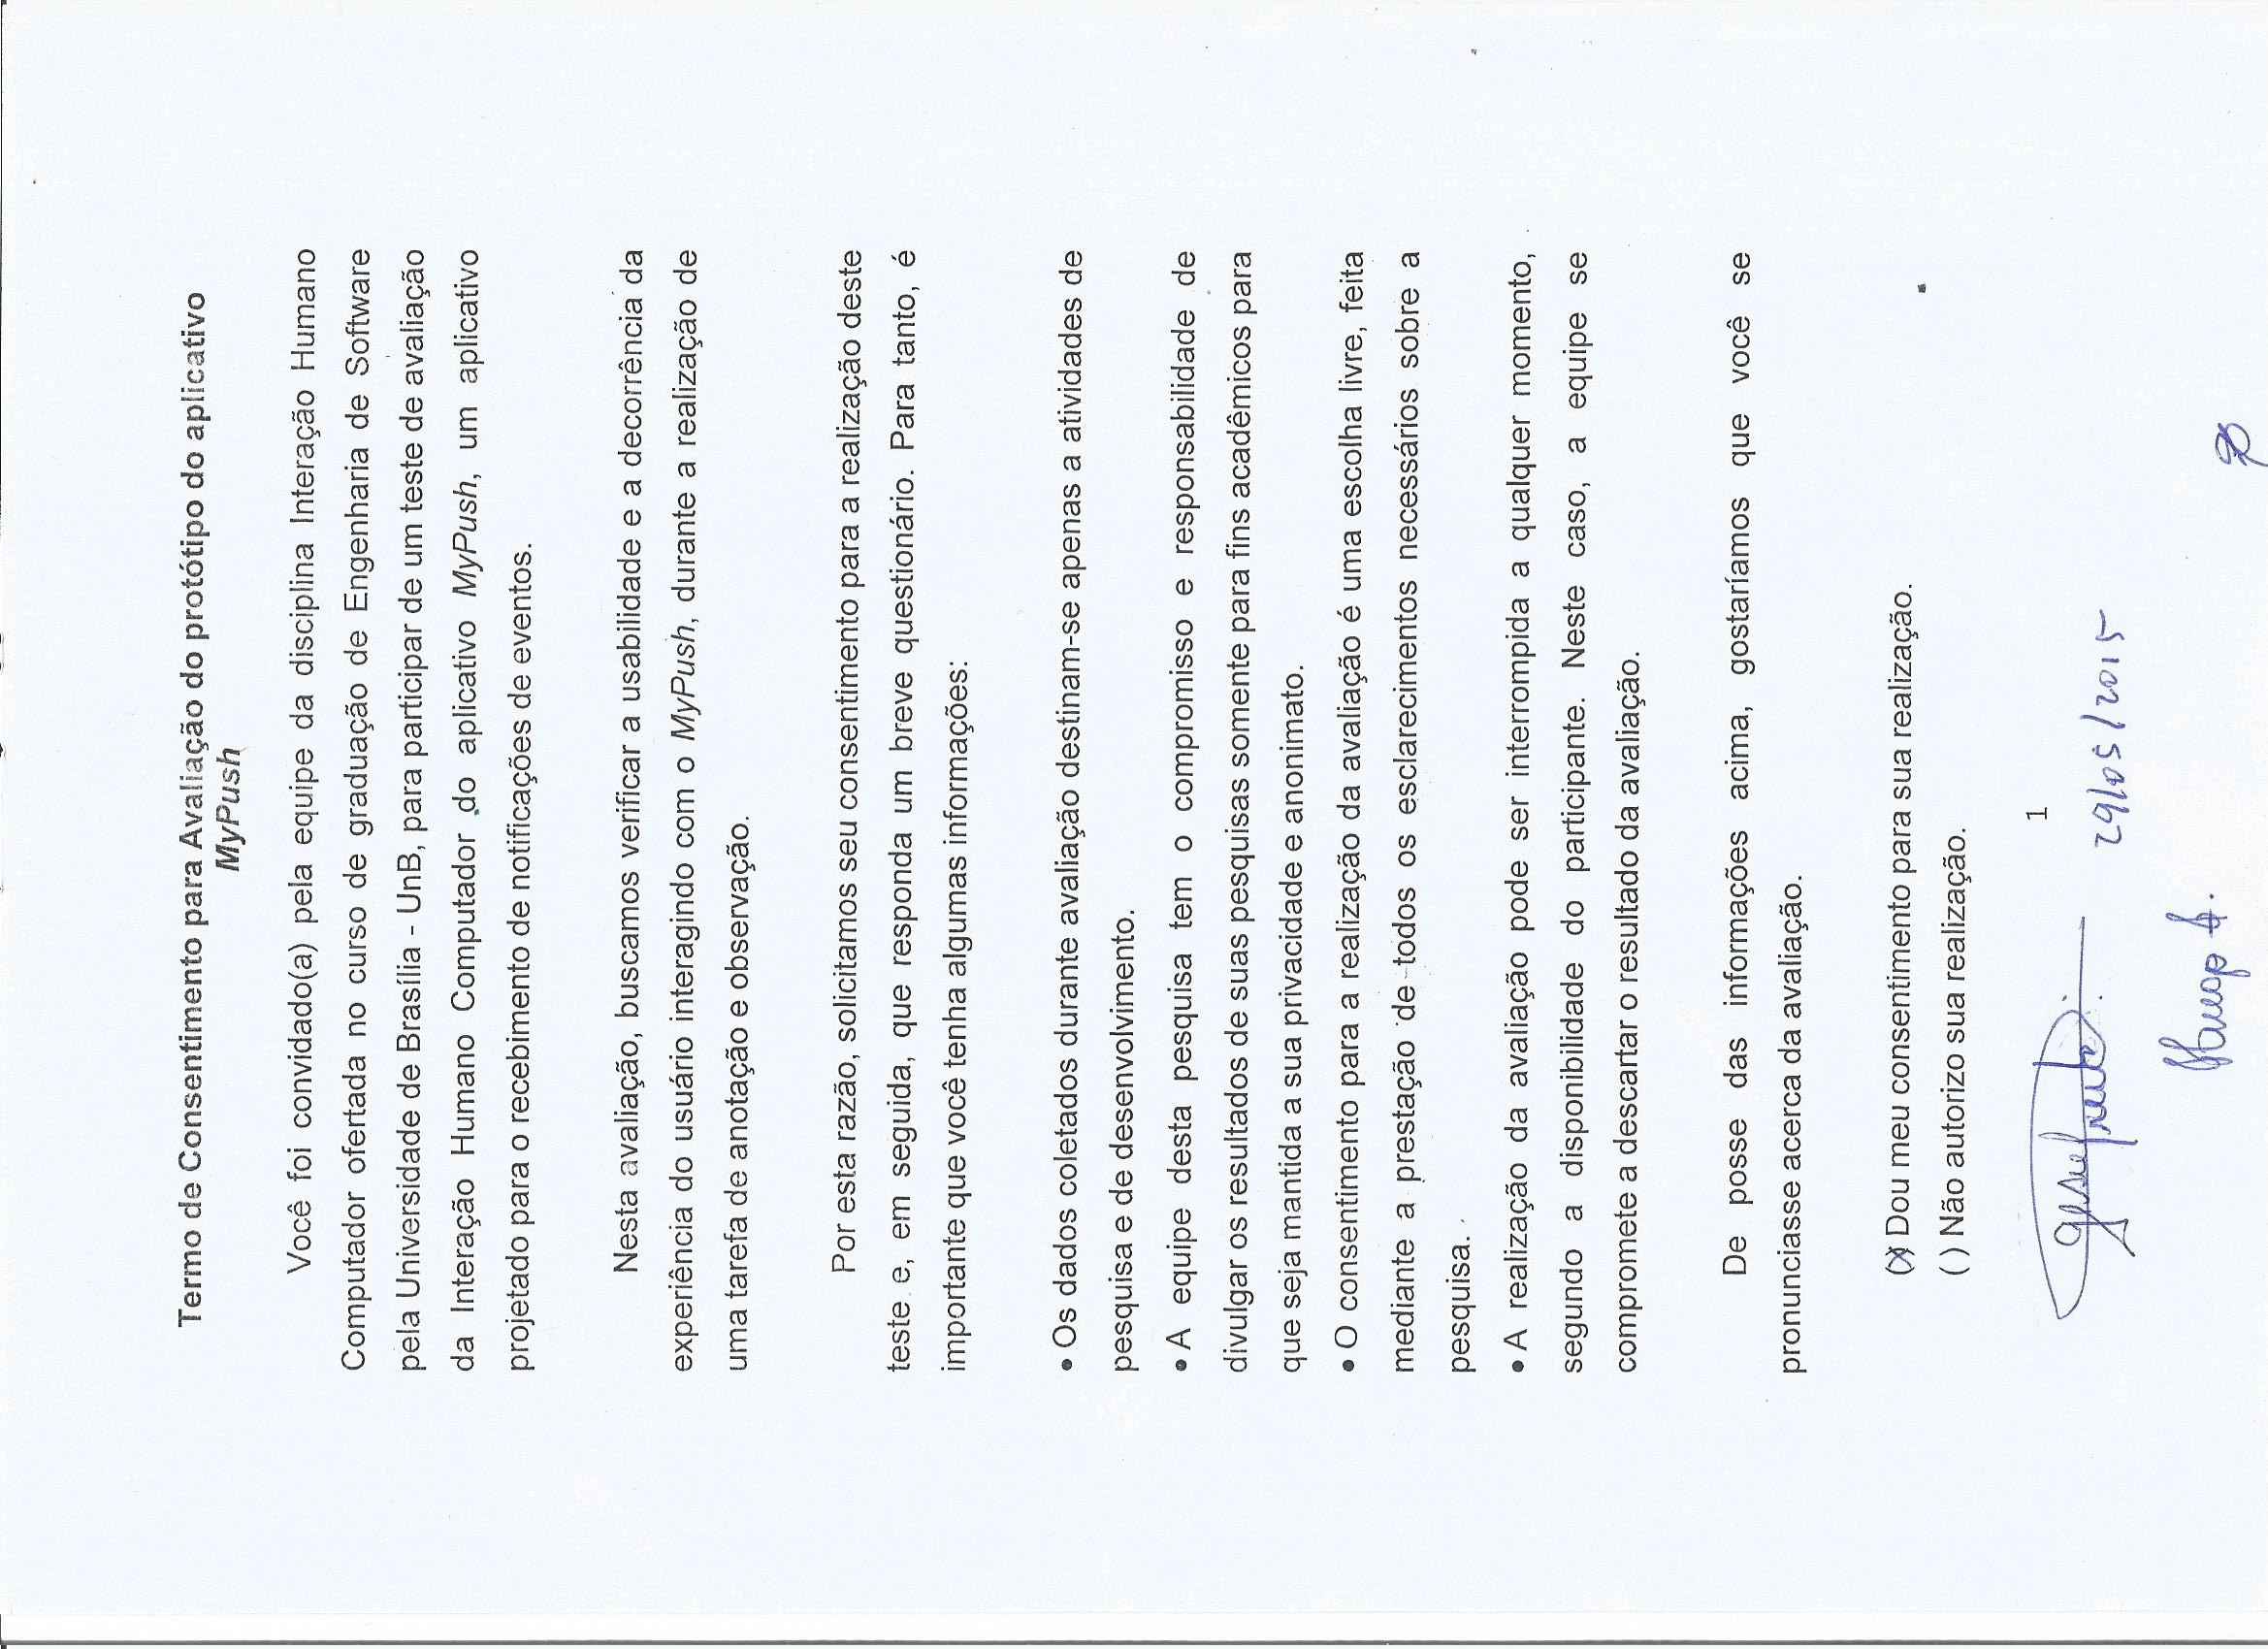
\includegraphics[scale=0.6, angle=-90]{editaveis/figuras/gesiel}
      \caption{Termo de consentimento assinado por um dos usuários que participaram da avaliação.}
      \label{termo_consentimento_1}
    \end{figure}
    
     \section*{Usuário 11}
    \begin{figure}[!htbp]
      \centering
      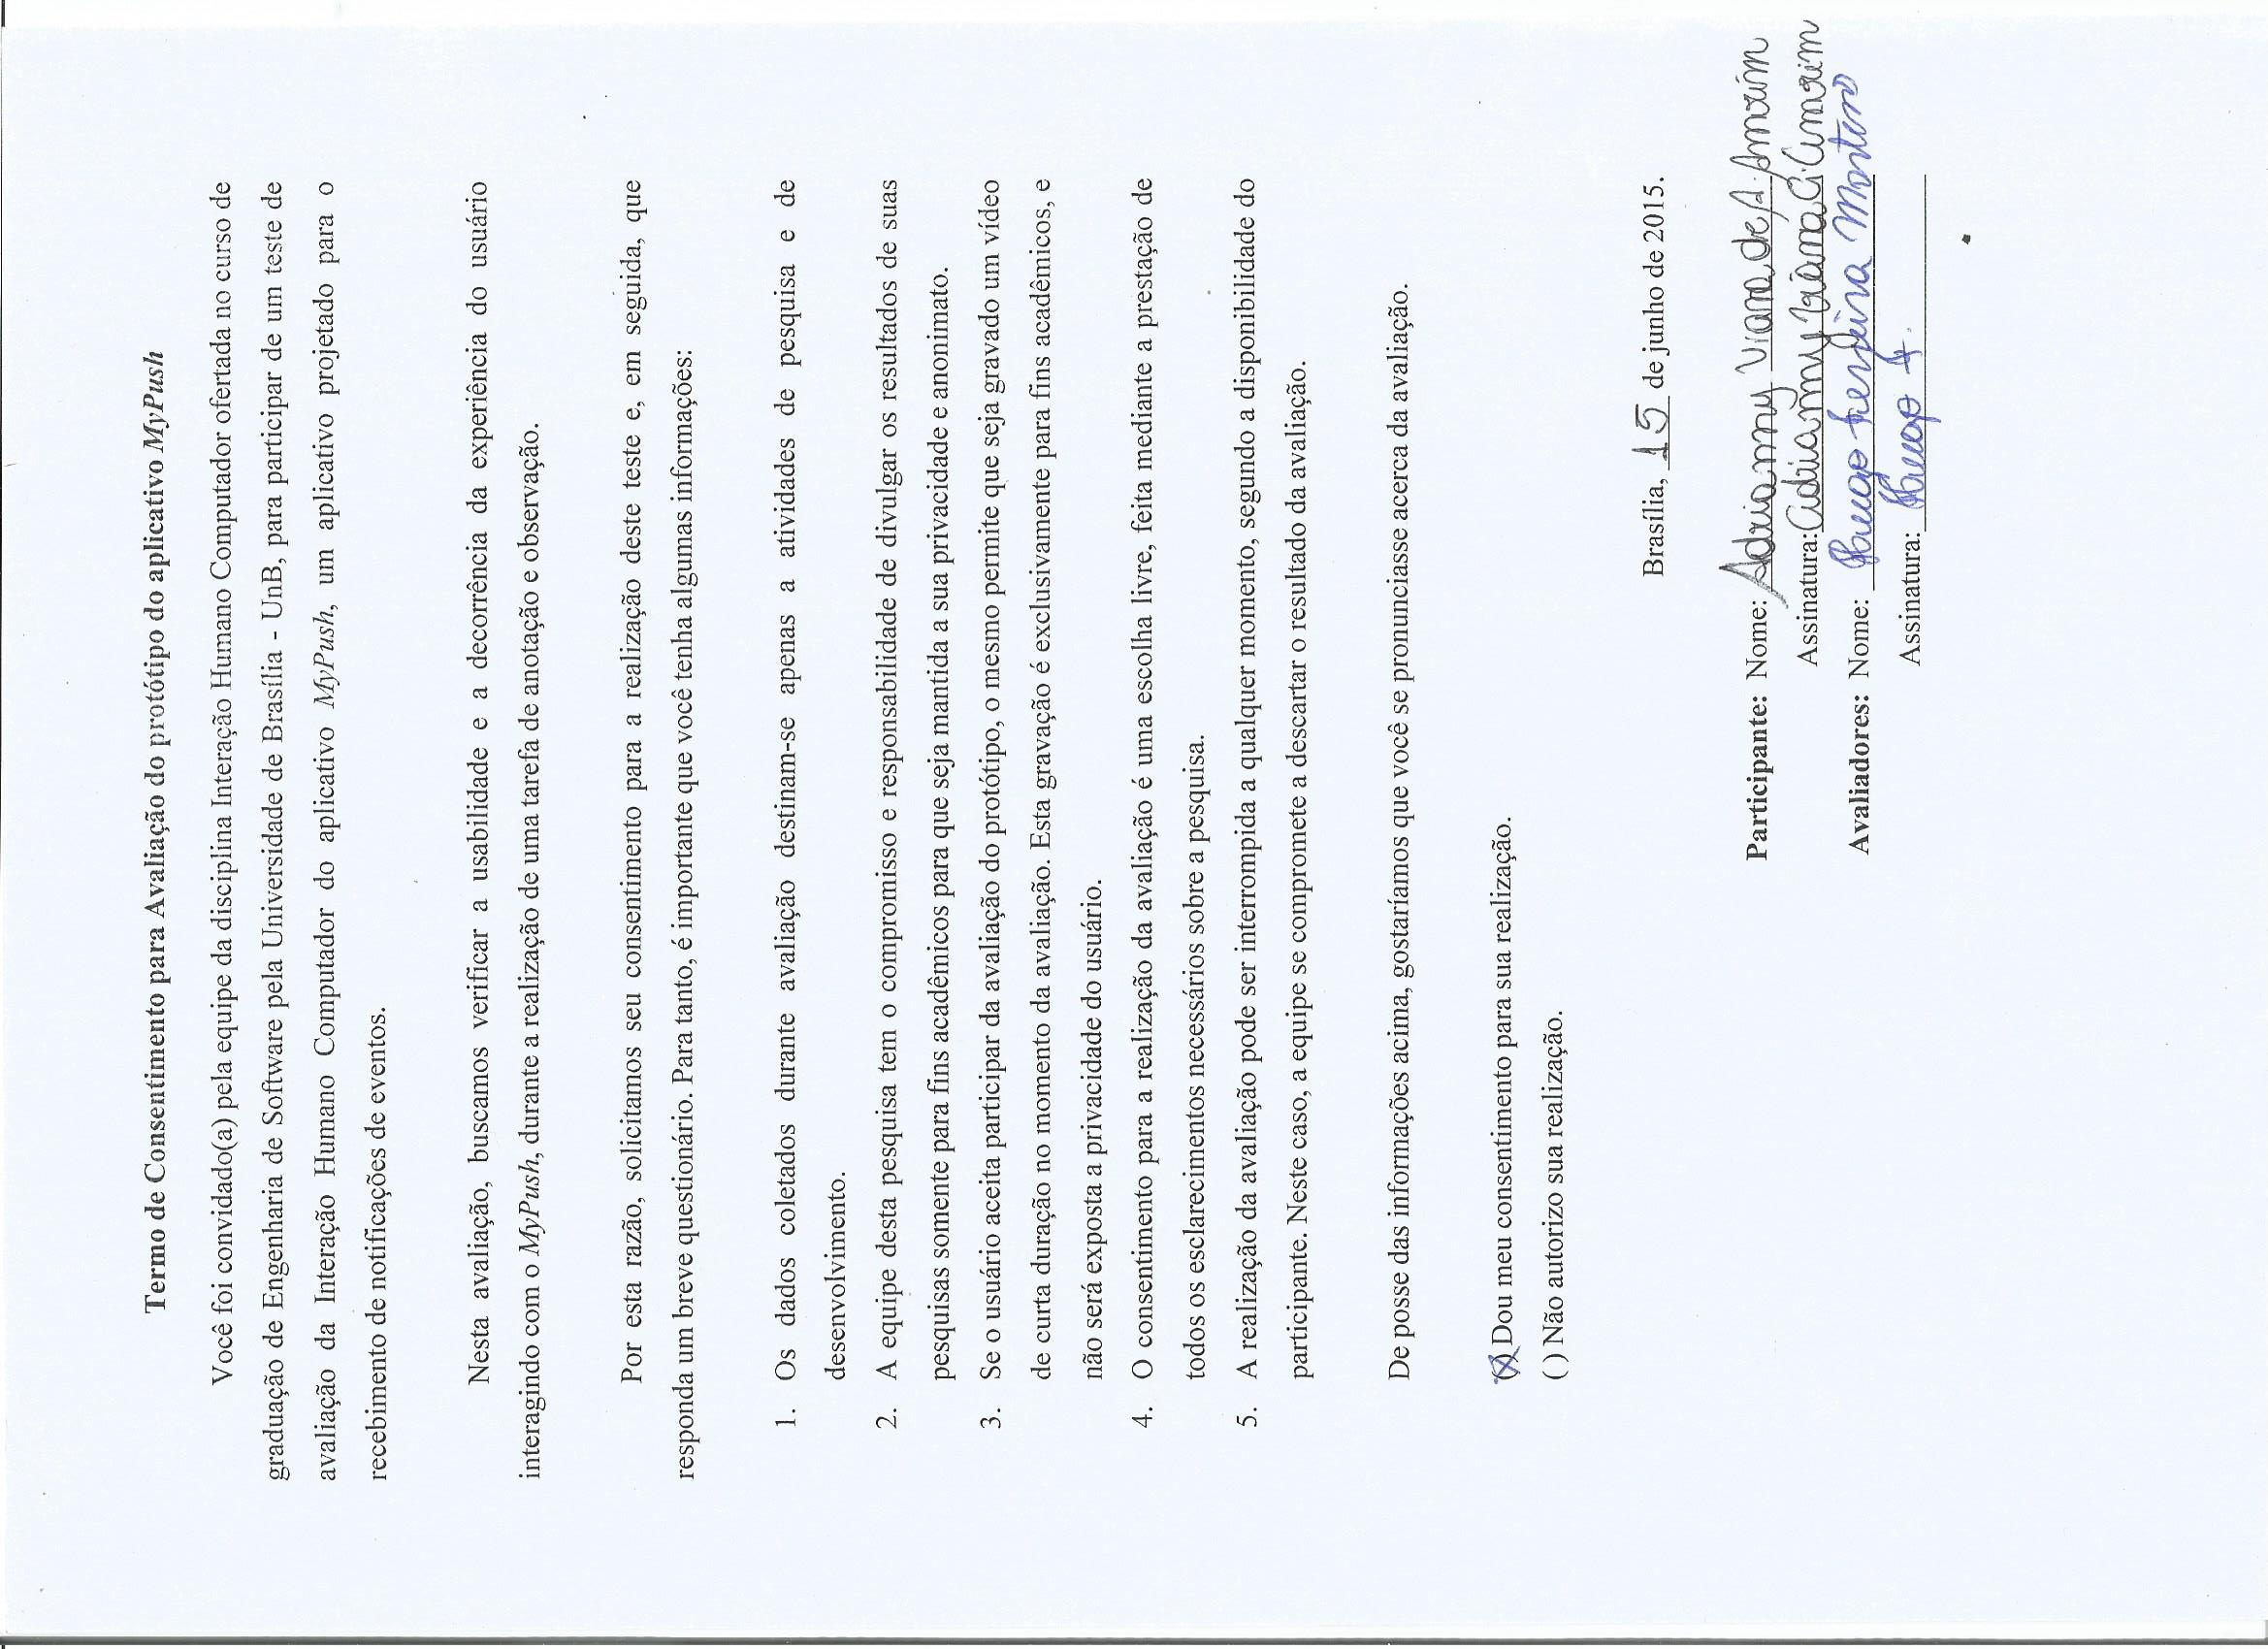
\includegraphics[scale=0.6, angle=-90]{editaveis/figuras/adrianny}
      \caption{Termo de consentimento assinado por um dos usuários que participaram da avaliação.}
      \label{termo_consentimento_1}
    \end{figure}
	
	
	 \section*{Usuário 12}
    \begin{figure}[!htbp]
      \centering
      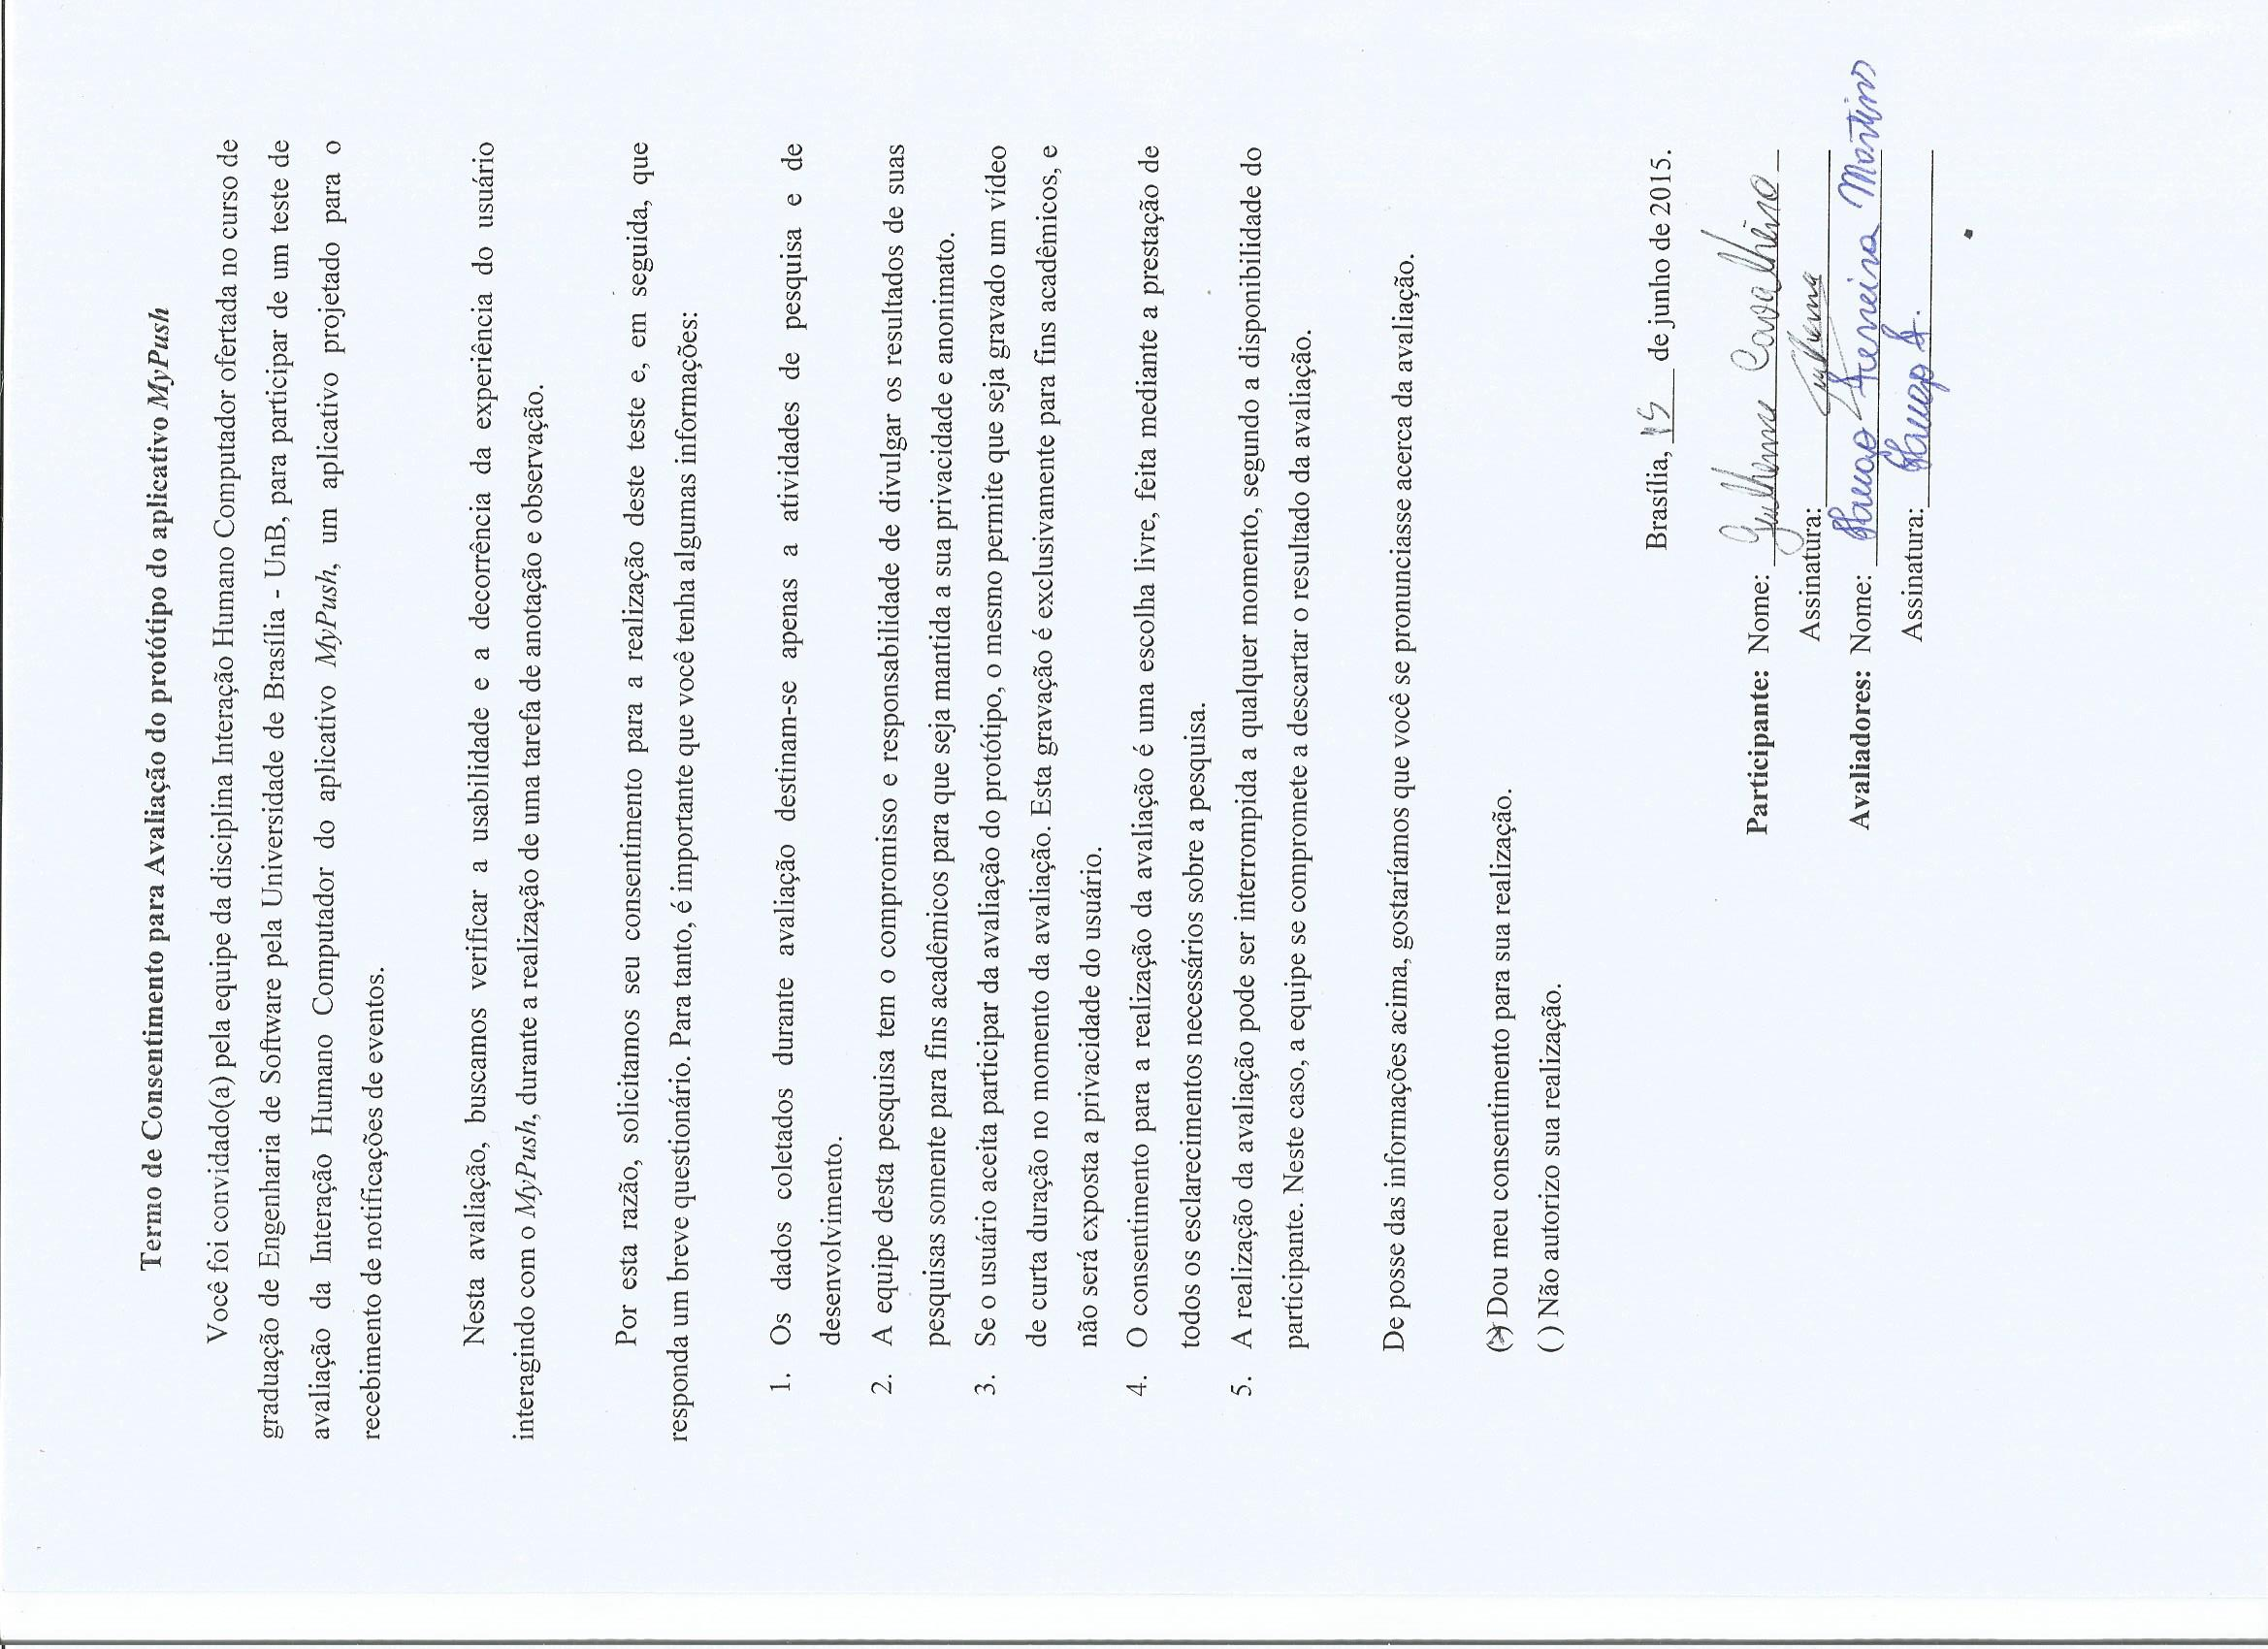
\includegraphics[scale=0.6, angle=-90]{editaveis/figuras/cavalheiro}
      \caption{Termo de consentimento assinado por um dos usuários que participaram da avaliação.}
      \label{termo_consentimento_1}
    \end{figure}
	
	
	 \section*{Usuário 13}
    \begin{figure}[!htbp]
      \centering
      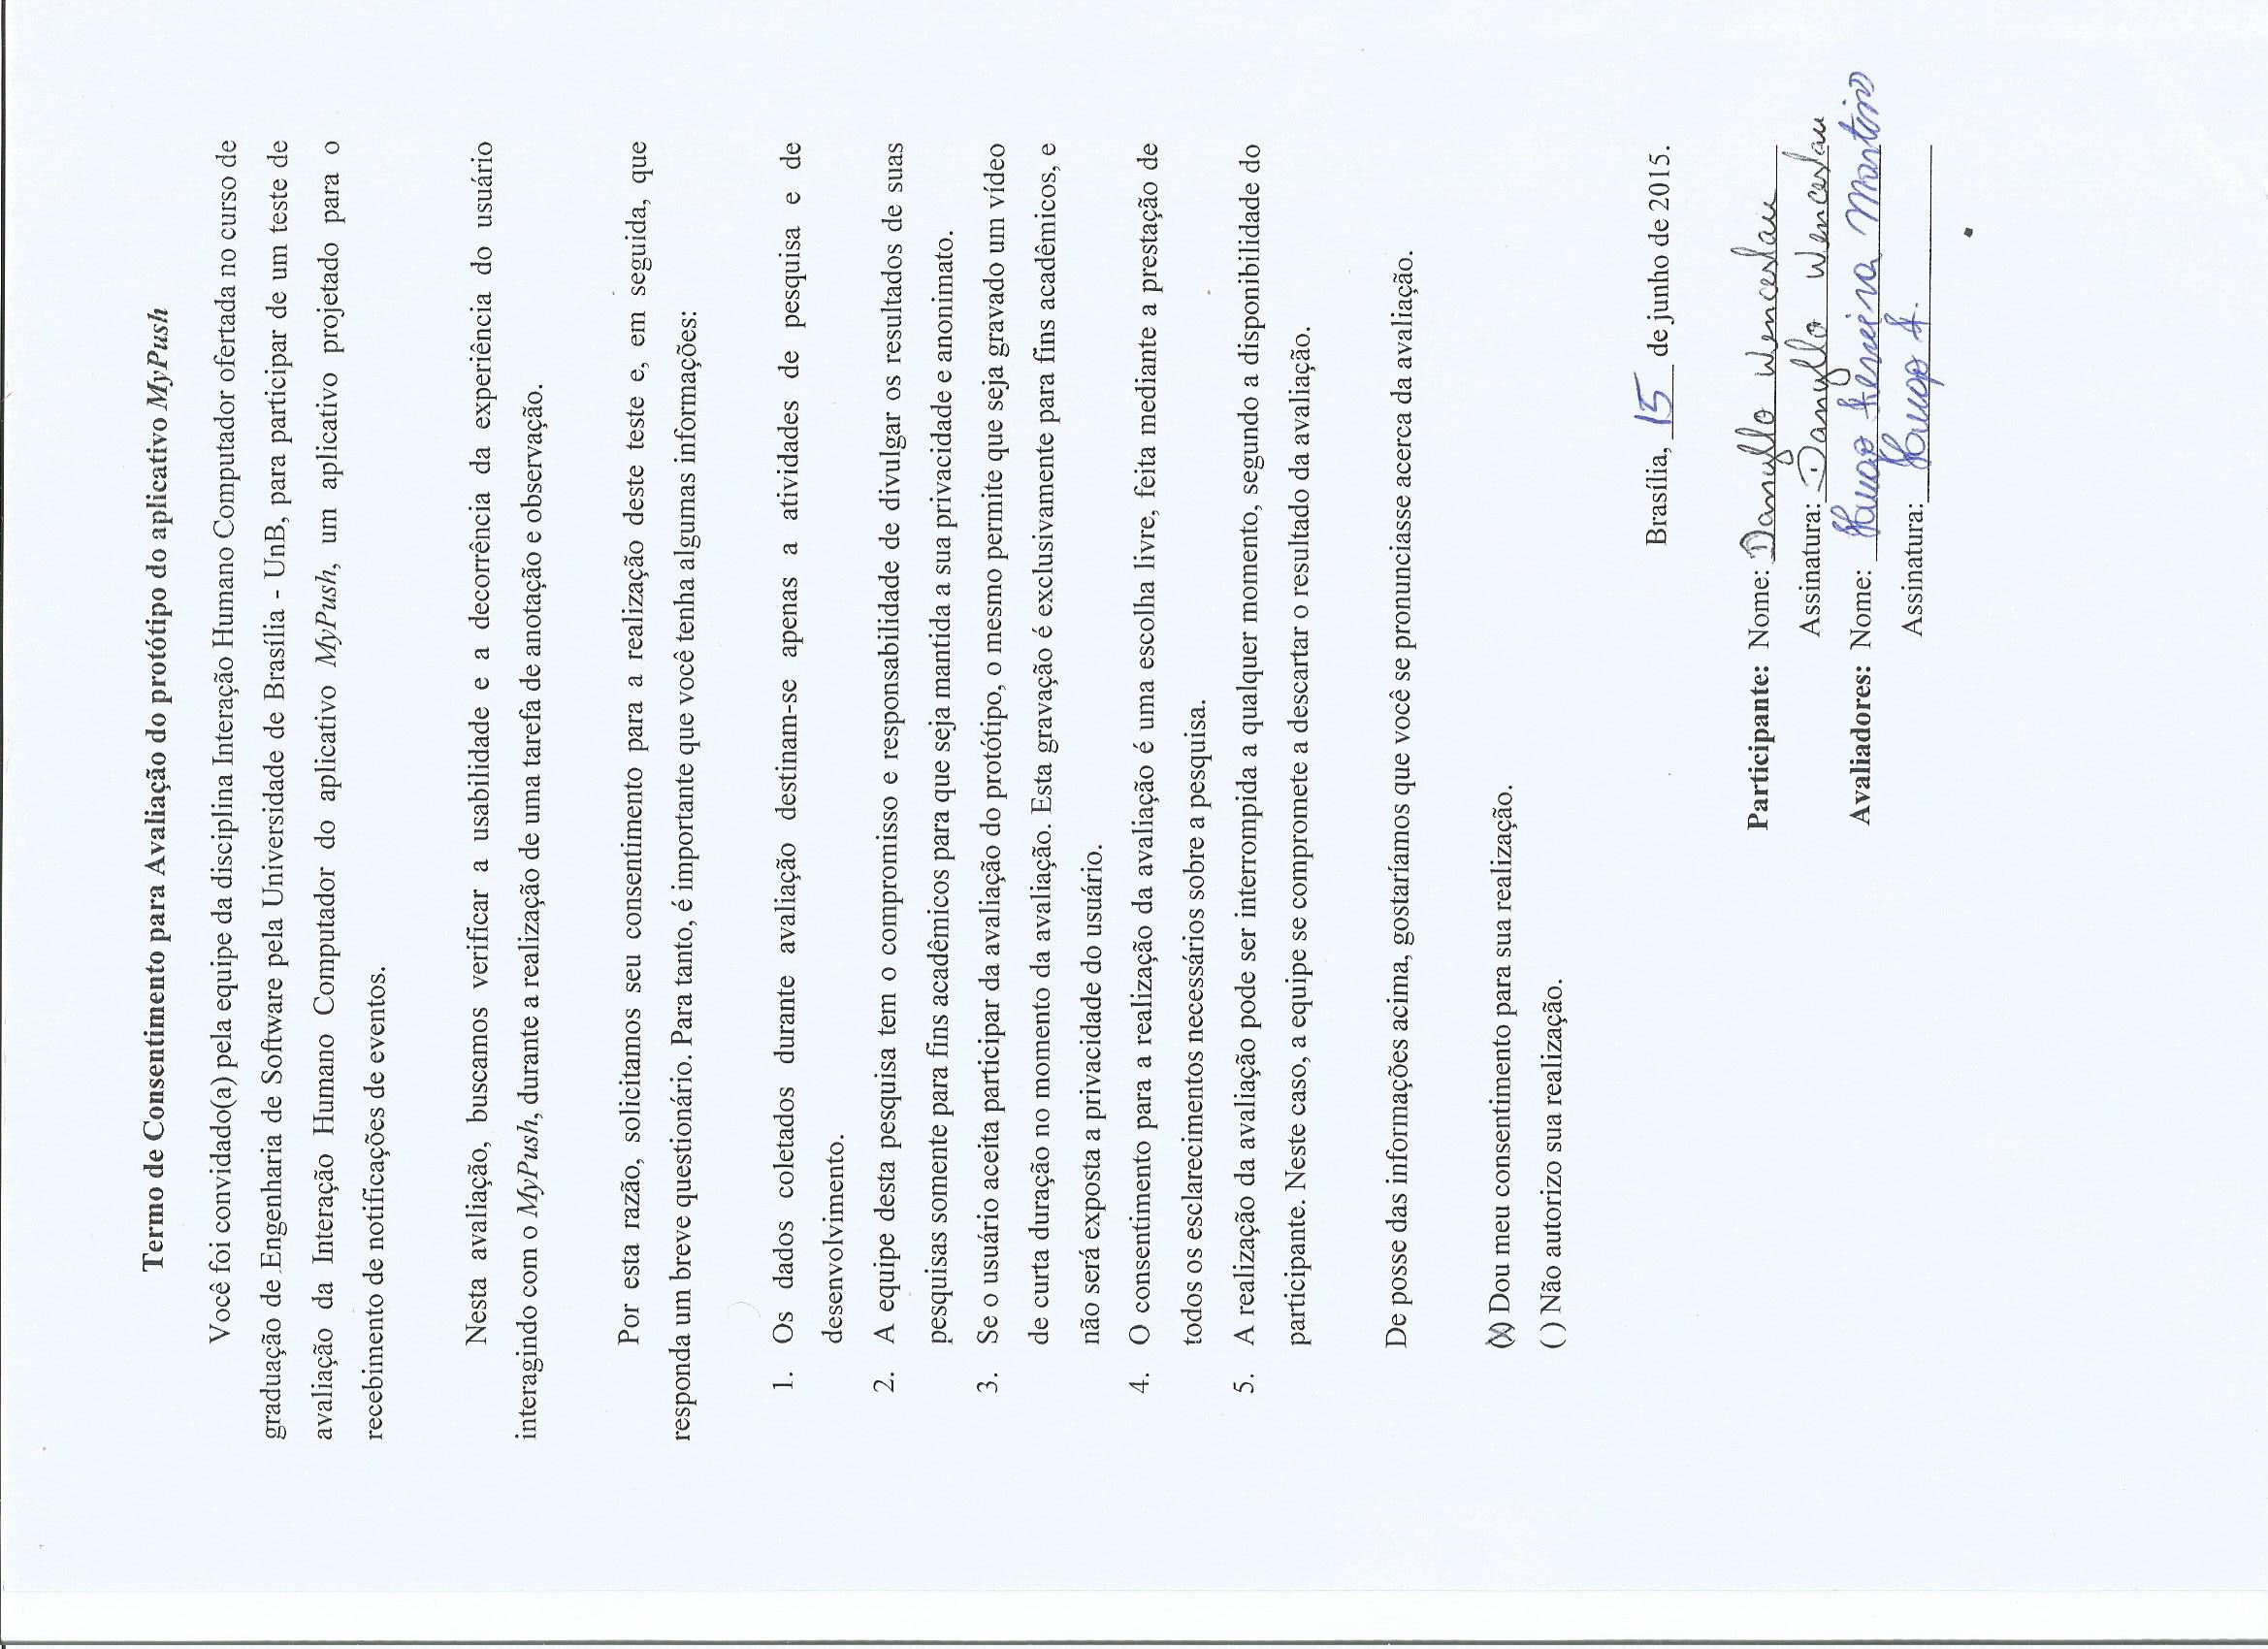
\includegraphics[scale=0.6, angle=-90]{editaveis/figuras/danilo}
      \caption{Termo de consentimento assinado por um dos usuários que participaram da avaliação.}
      \label{termo_consentimento_1}
    \end{figure}
	
	
	 \section*{Usuário 14}
    \begin{figure}[!htbp]
      \centering
      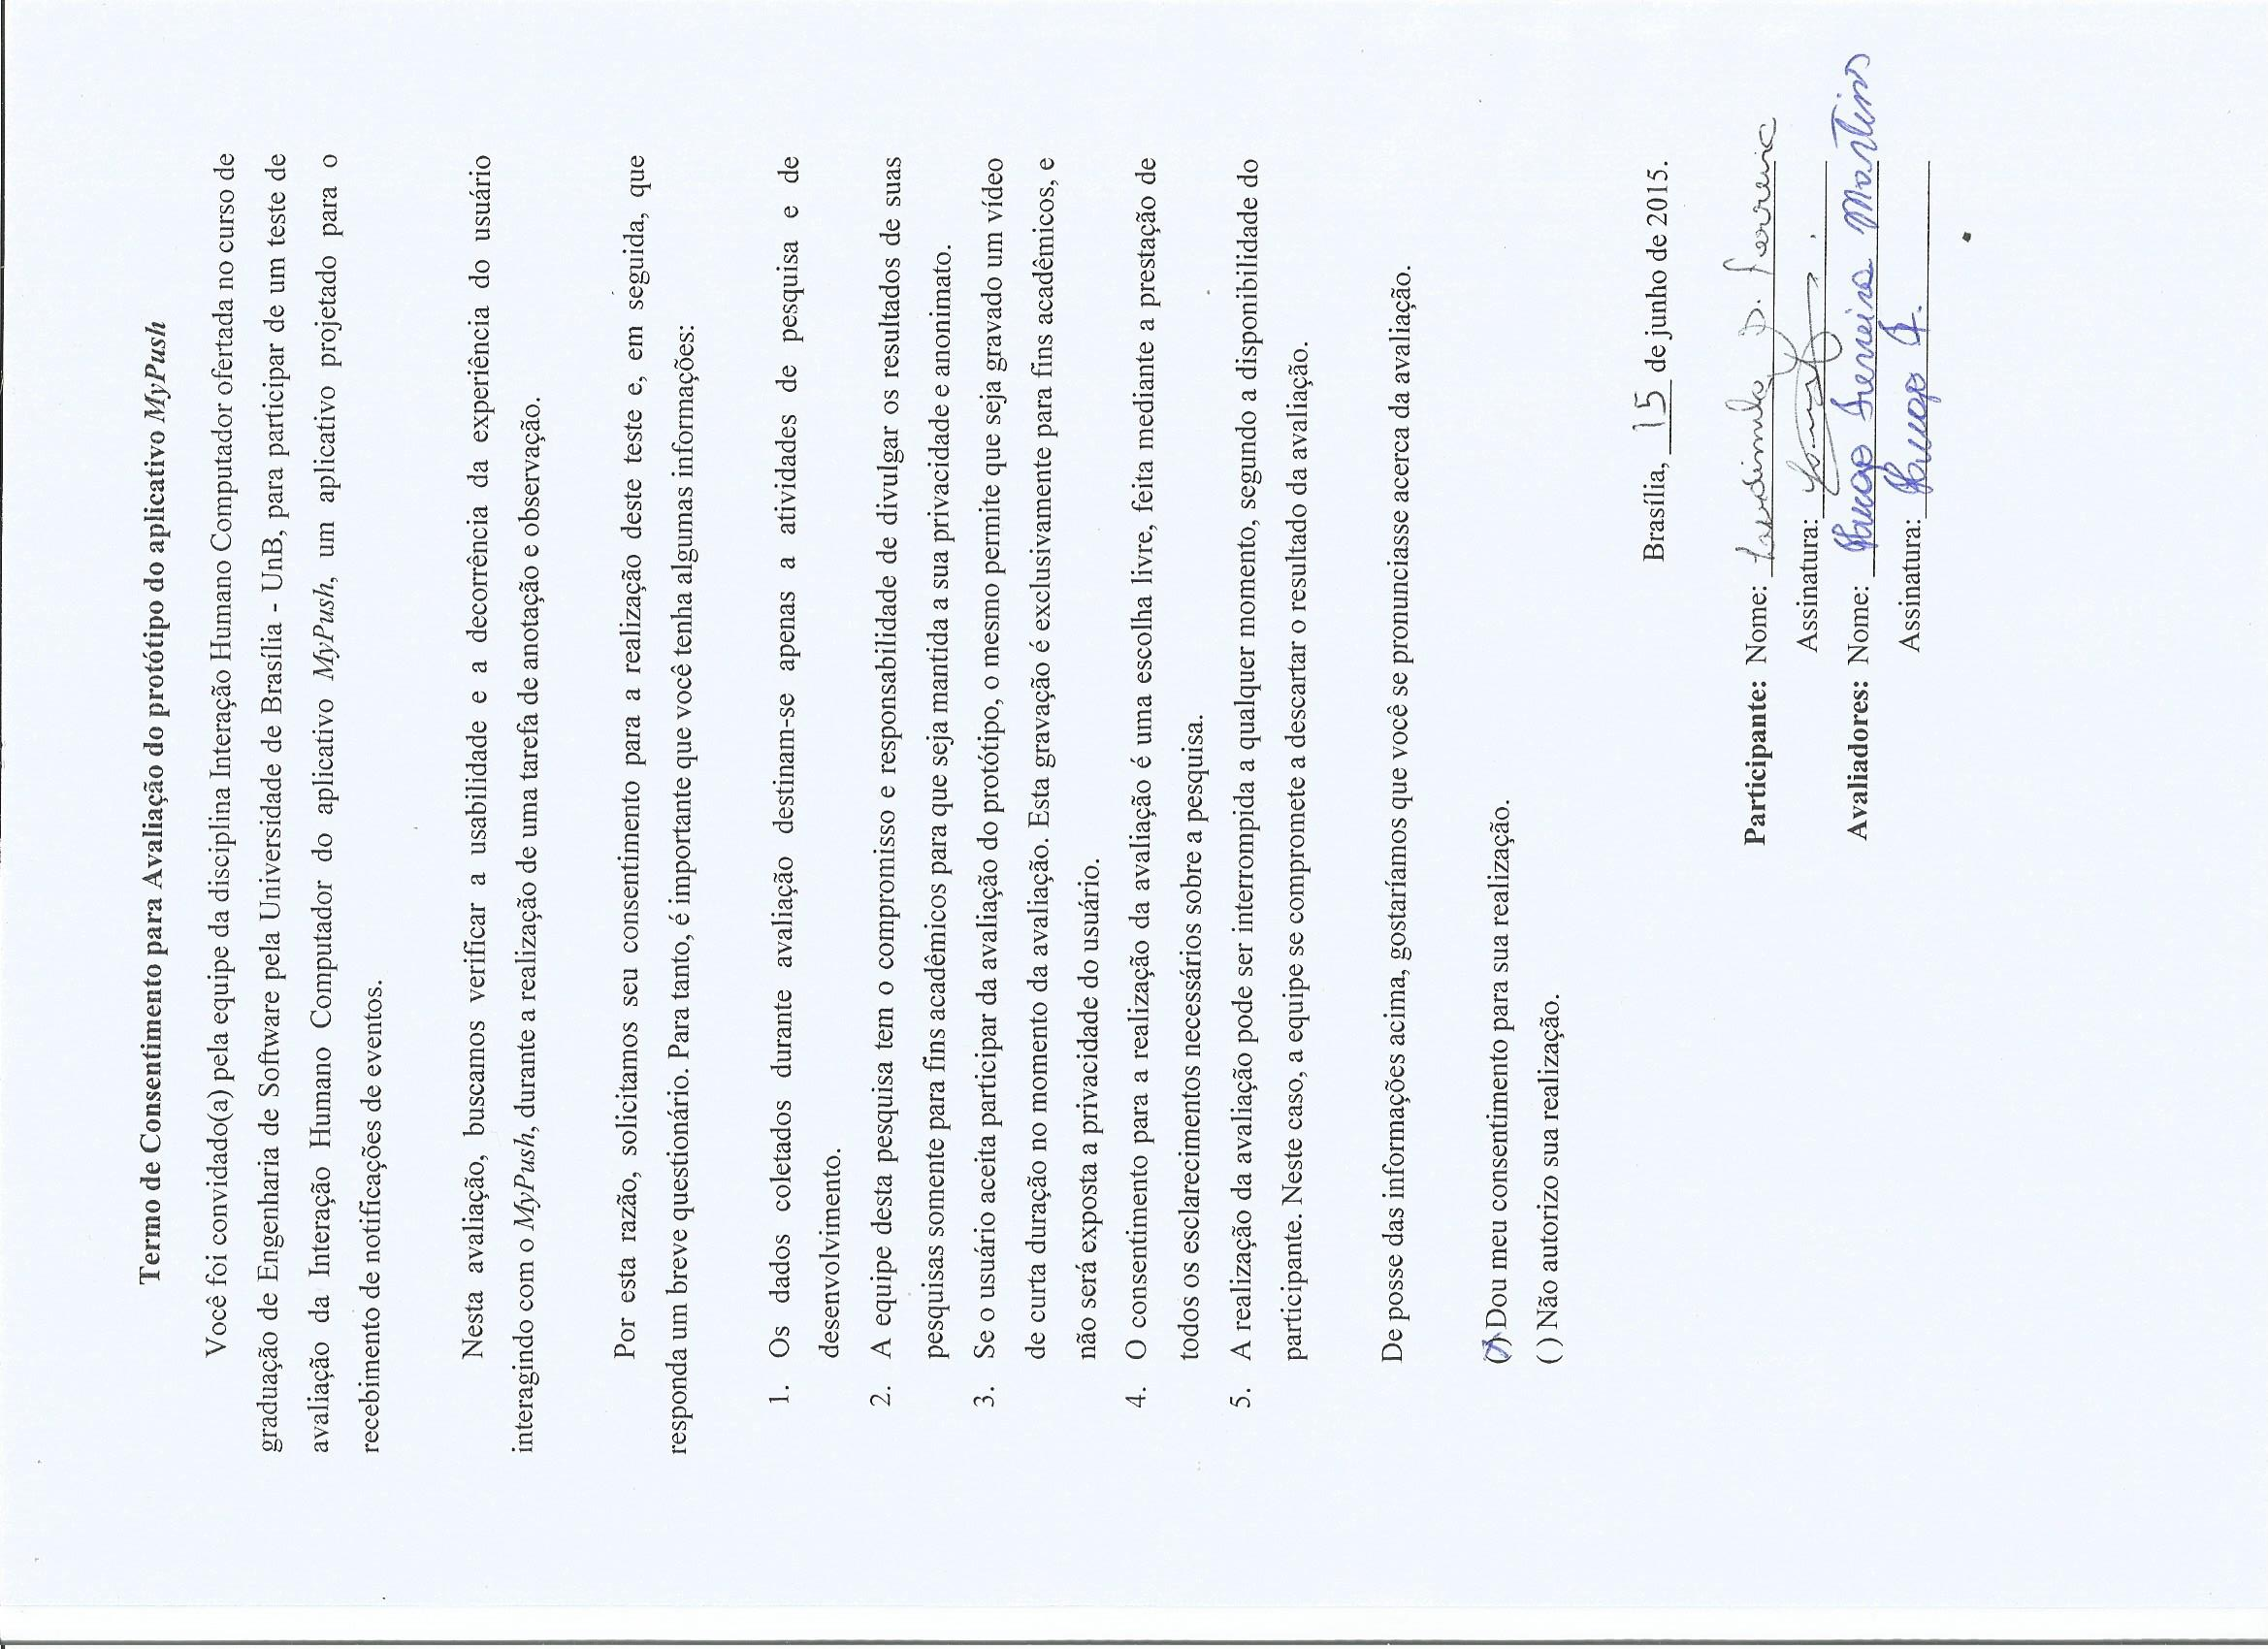
\includegraphics[scale=0.6, angle=-90]{editaveis/figuras/ludimila}
      \caption{Termo de consentimento assinado por um dos usuários que participaram da avaliação.}
      \label{termo_consentimento_1}
    \end{figure}
	
	
	 \section*{Usuário 15}
    \begin{figure}[!htbp]
      \centering
      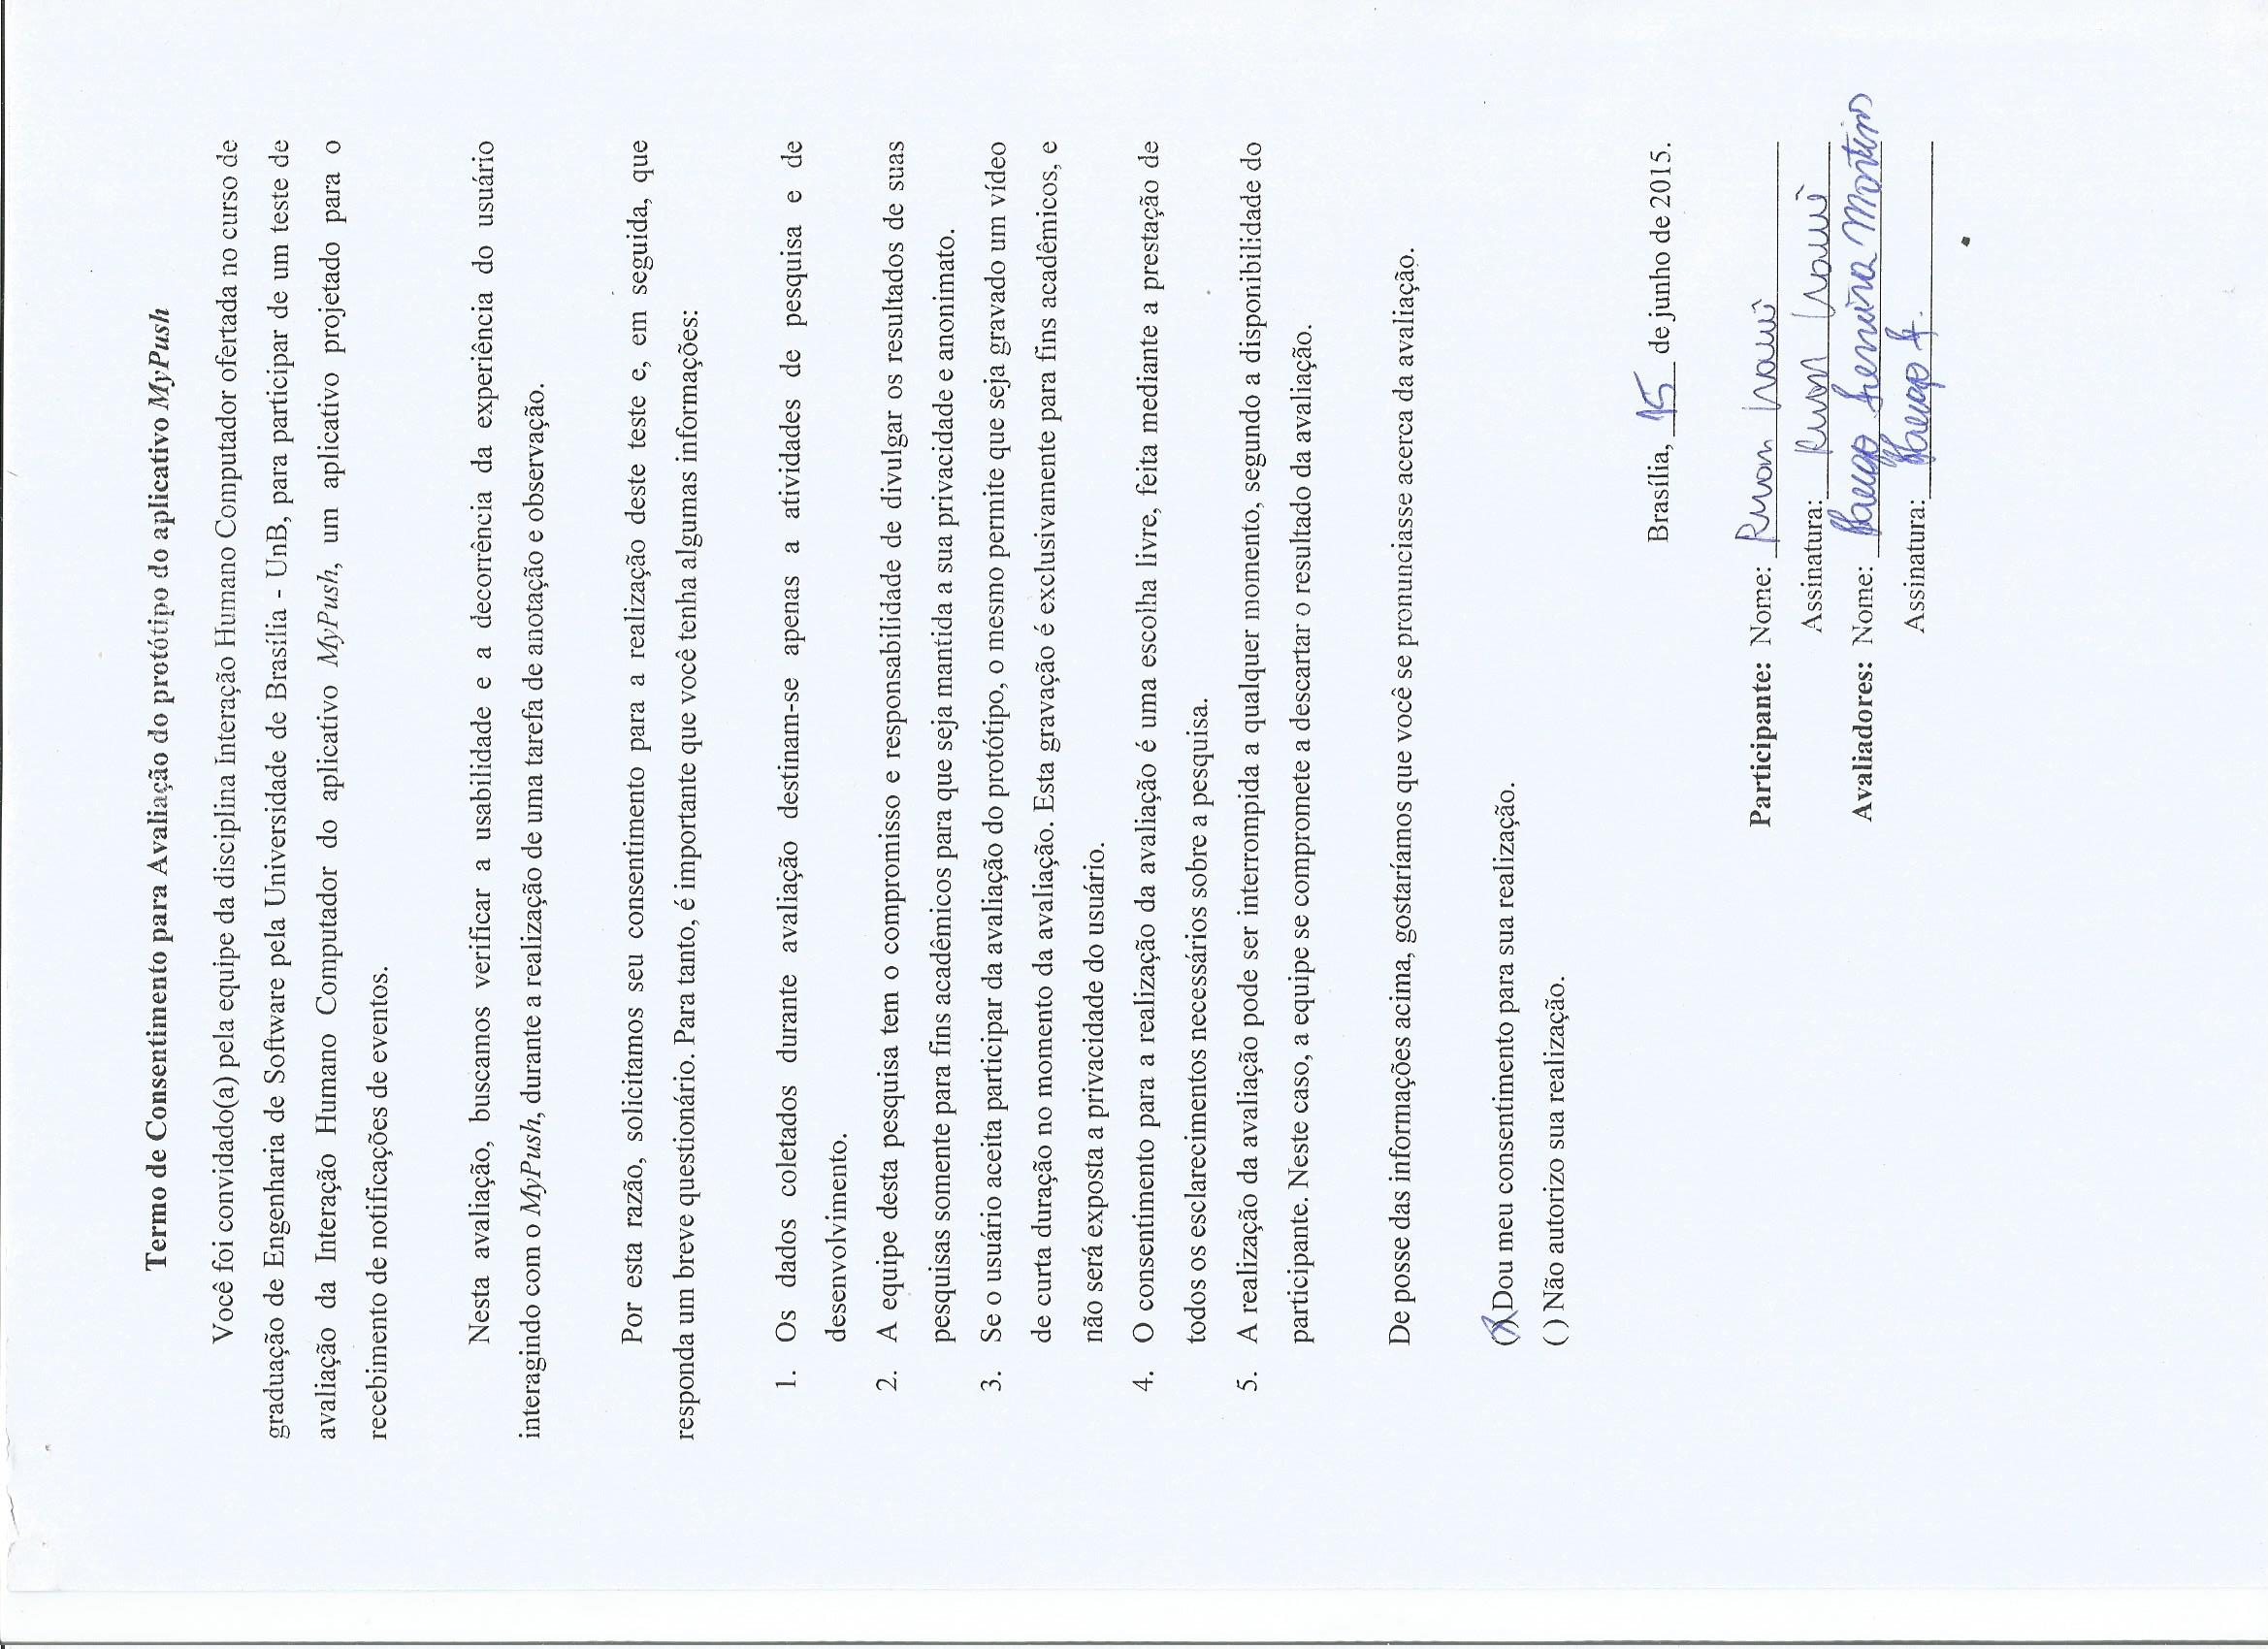
\includegraphics[scale=0.6, angle=-90]{editaveis/figuras/ruan}
      \caption{Termo de consentimento assinado por um dos usuários que participaram da avaliação.}
      \label{termo_consentimento_1}
    \end{figure}
    
    \section*{Usuário 16}
    \begin{figure}[!htbp]
      \centering
      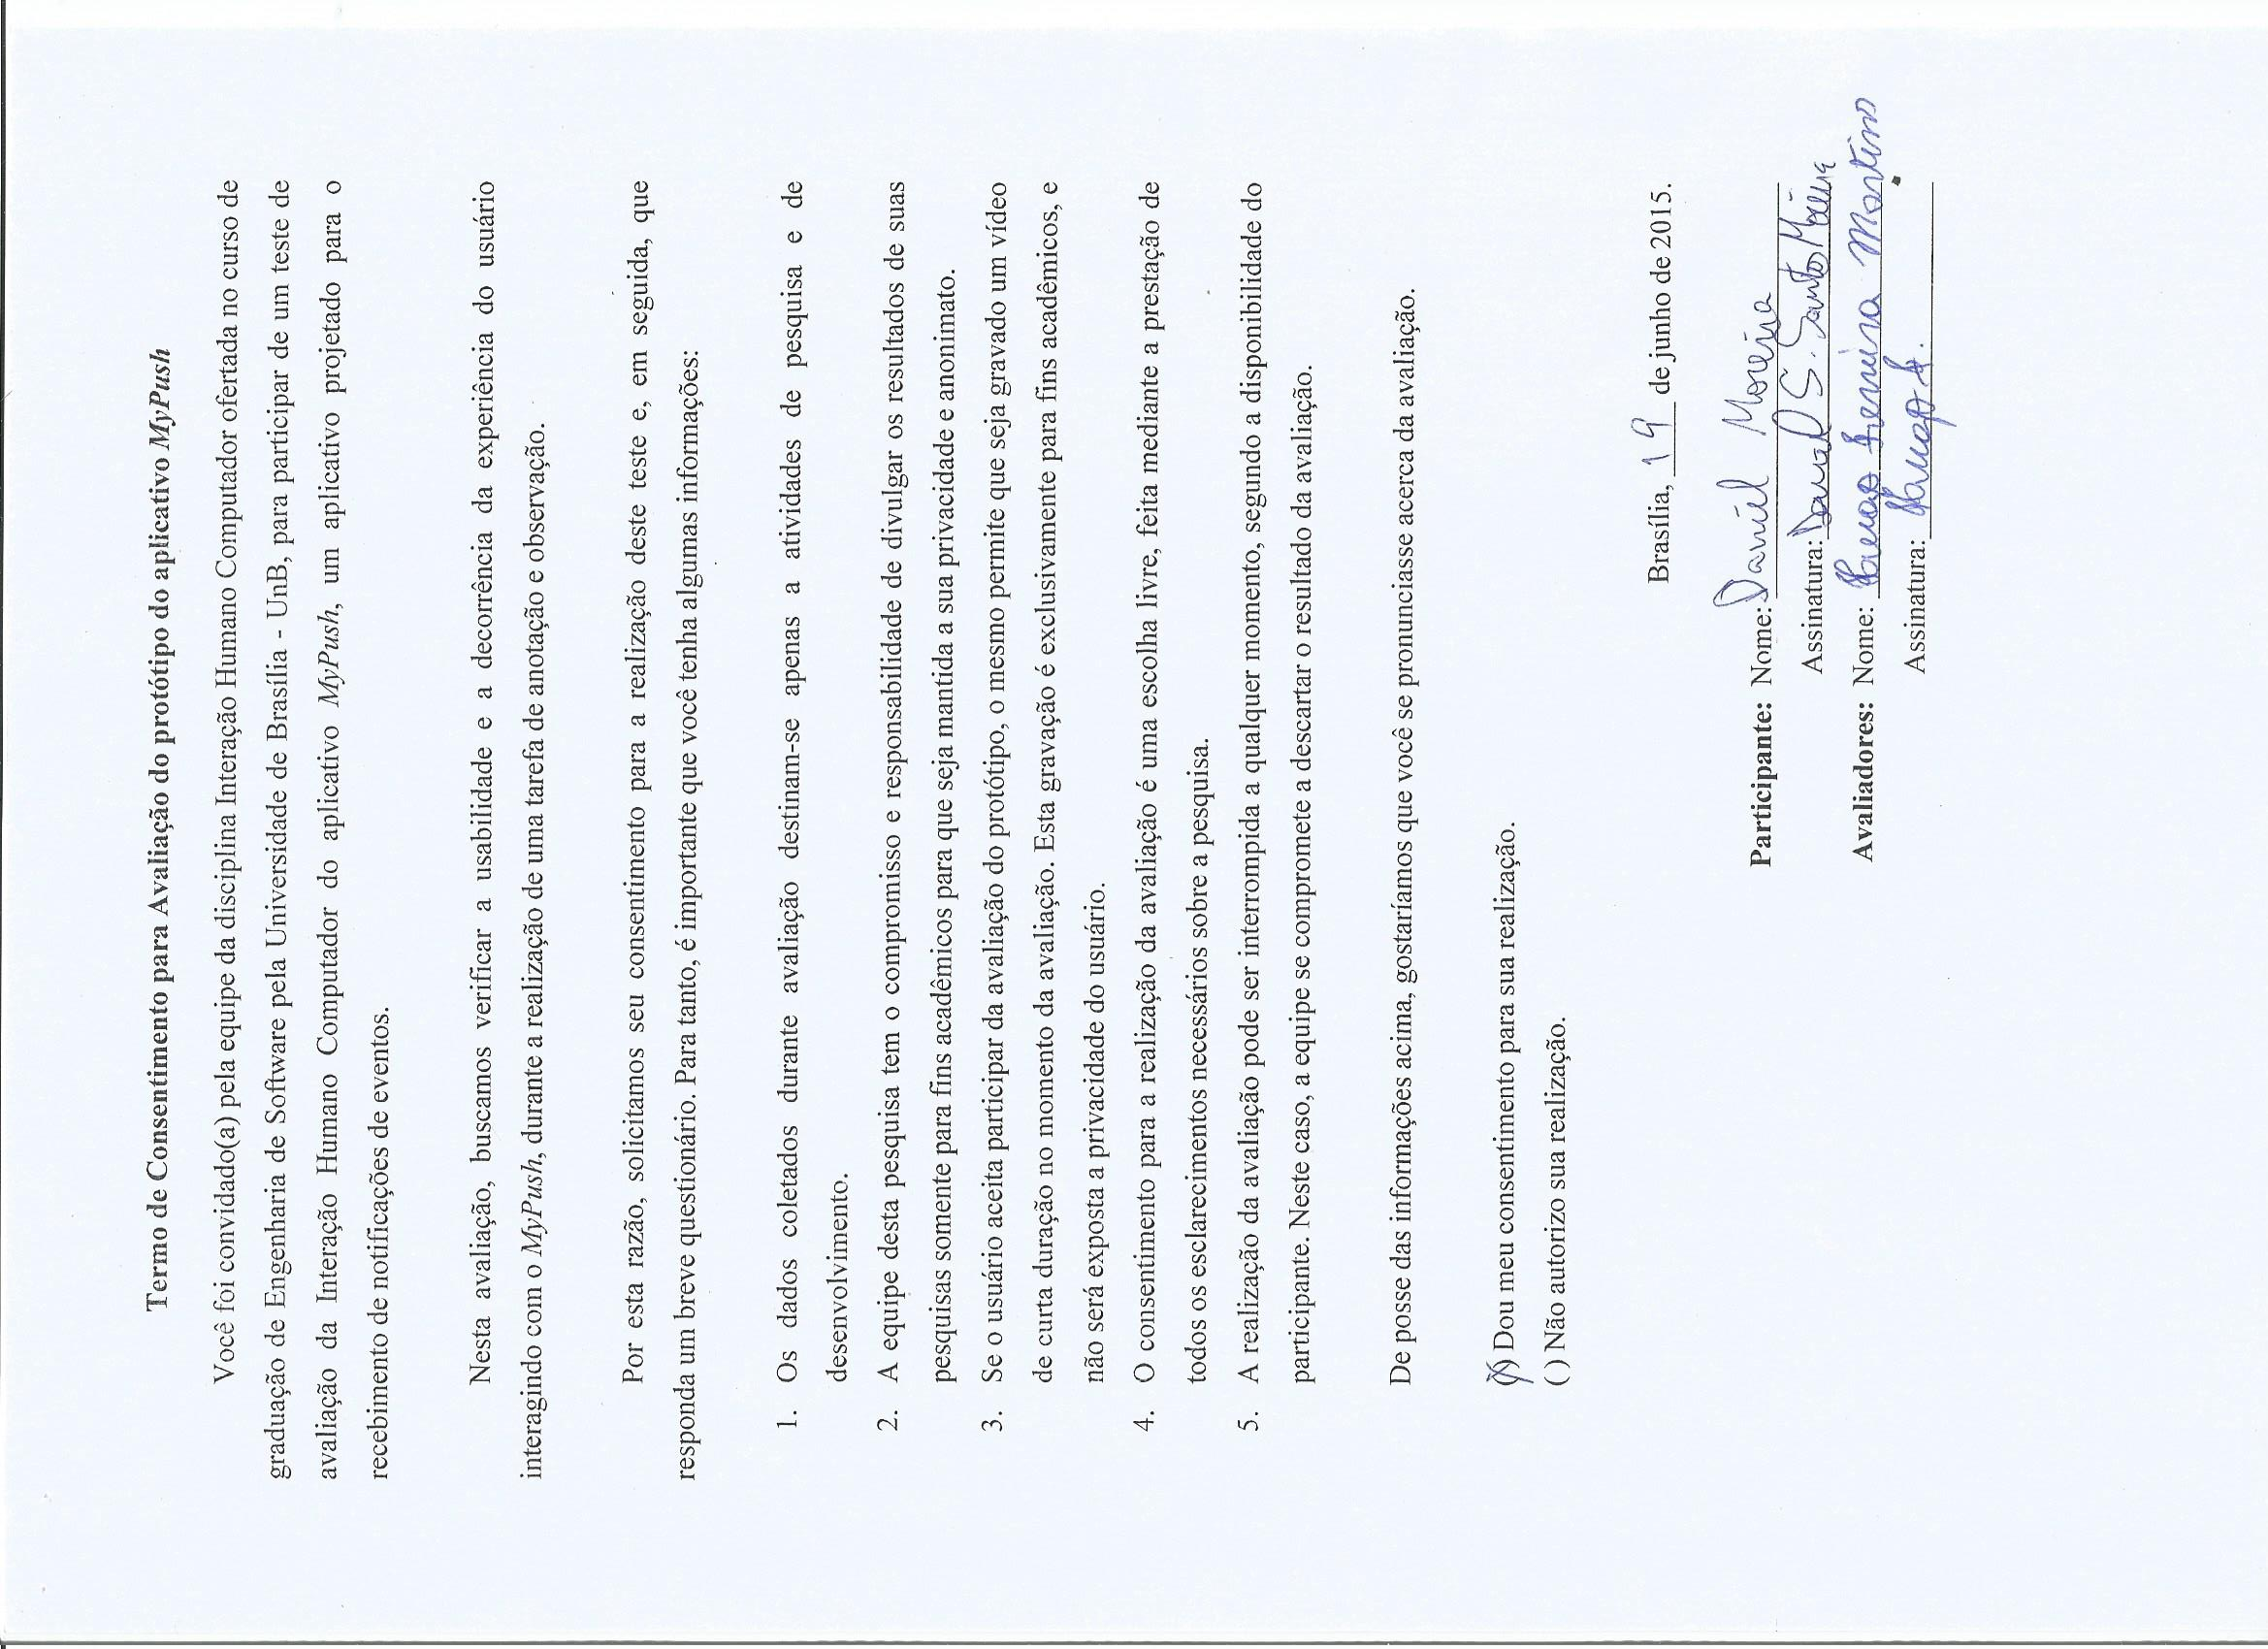
\includegraphics[scale=0.6, angle=-90]{editaveis/figuras/daniel}
      \caption{Termo de consentimento assinado por um dos usuários que participaram da avaliação.}
      \label{termo_consentimento_1}
    \end{figure}
    
    \section*{Usuário 17}
    \begin{figure}[!htbp]
      \centering
      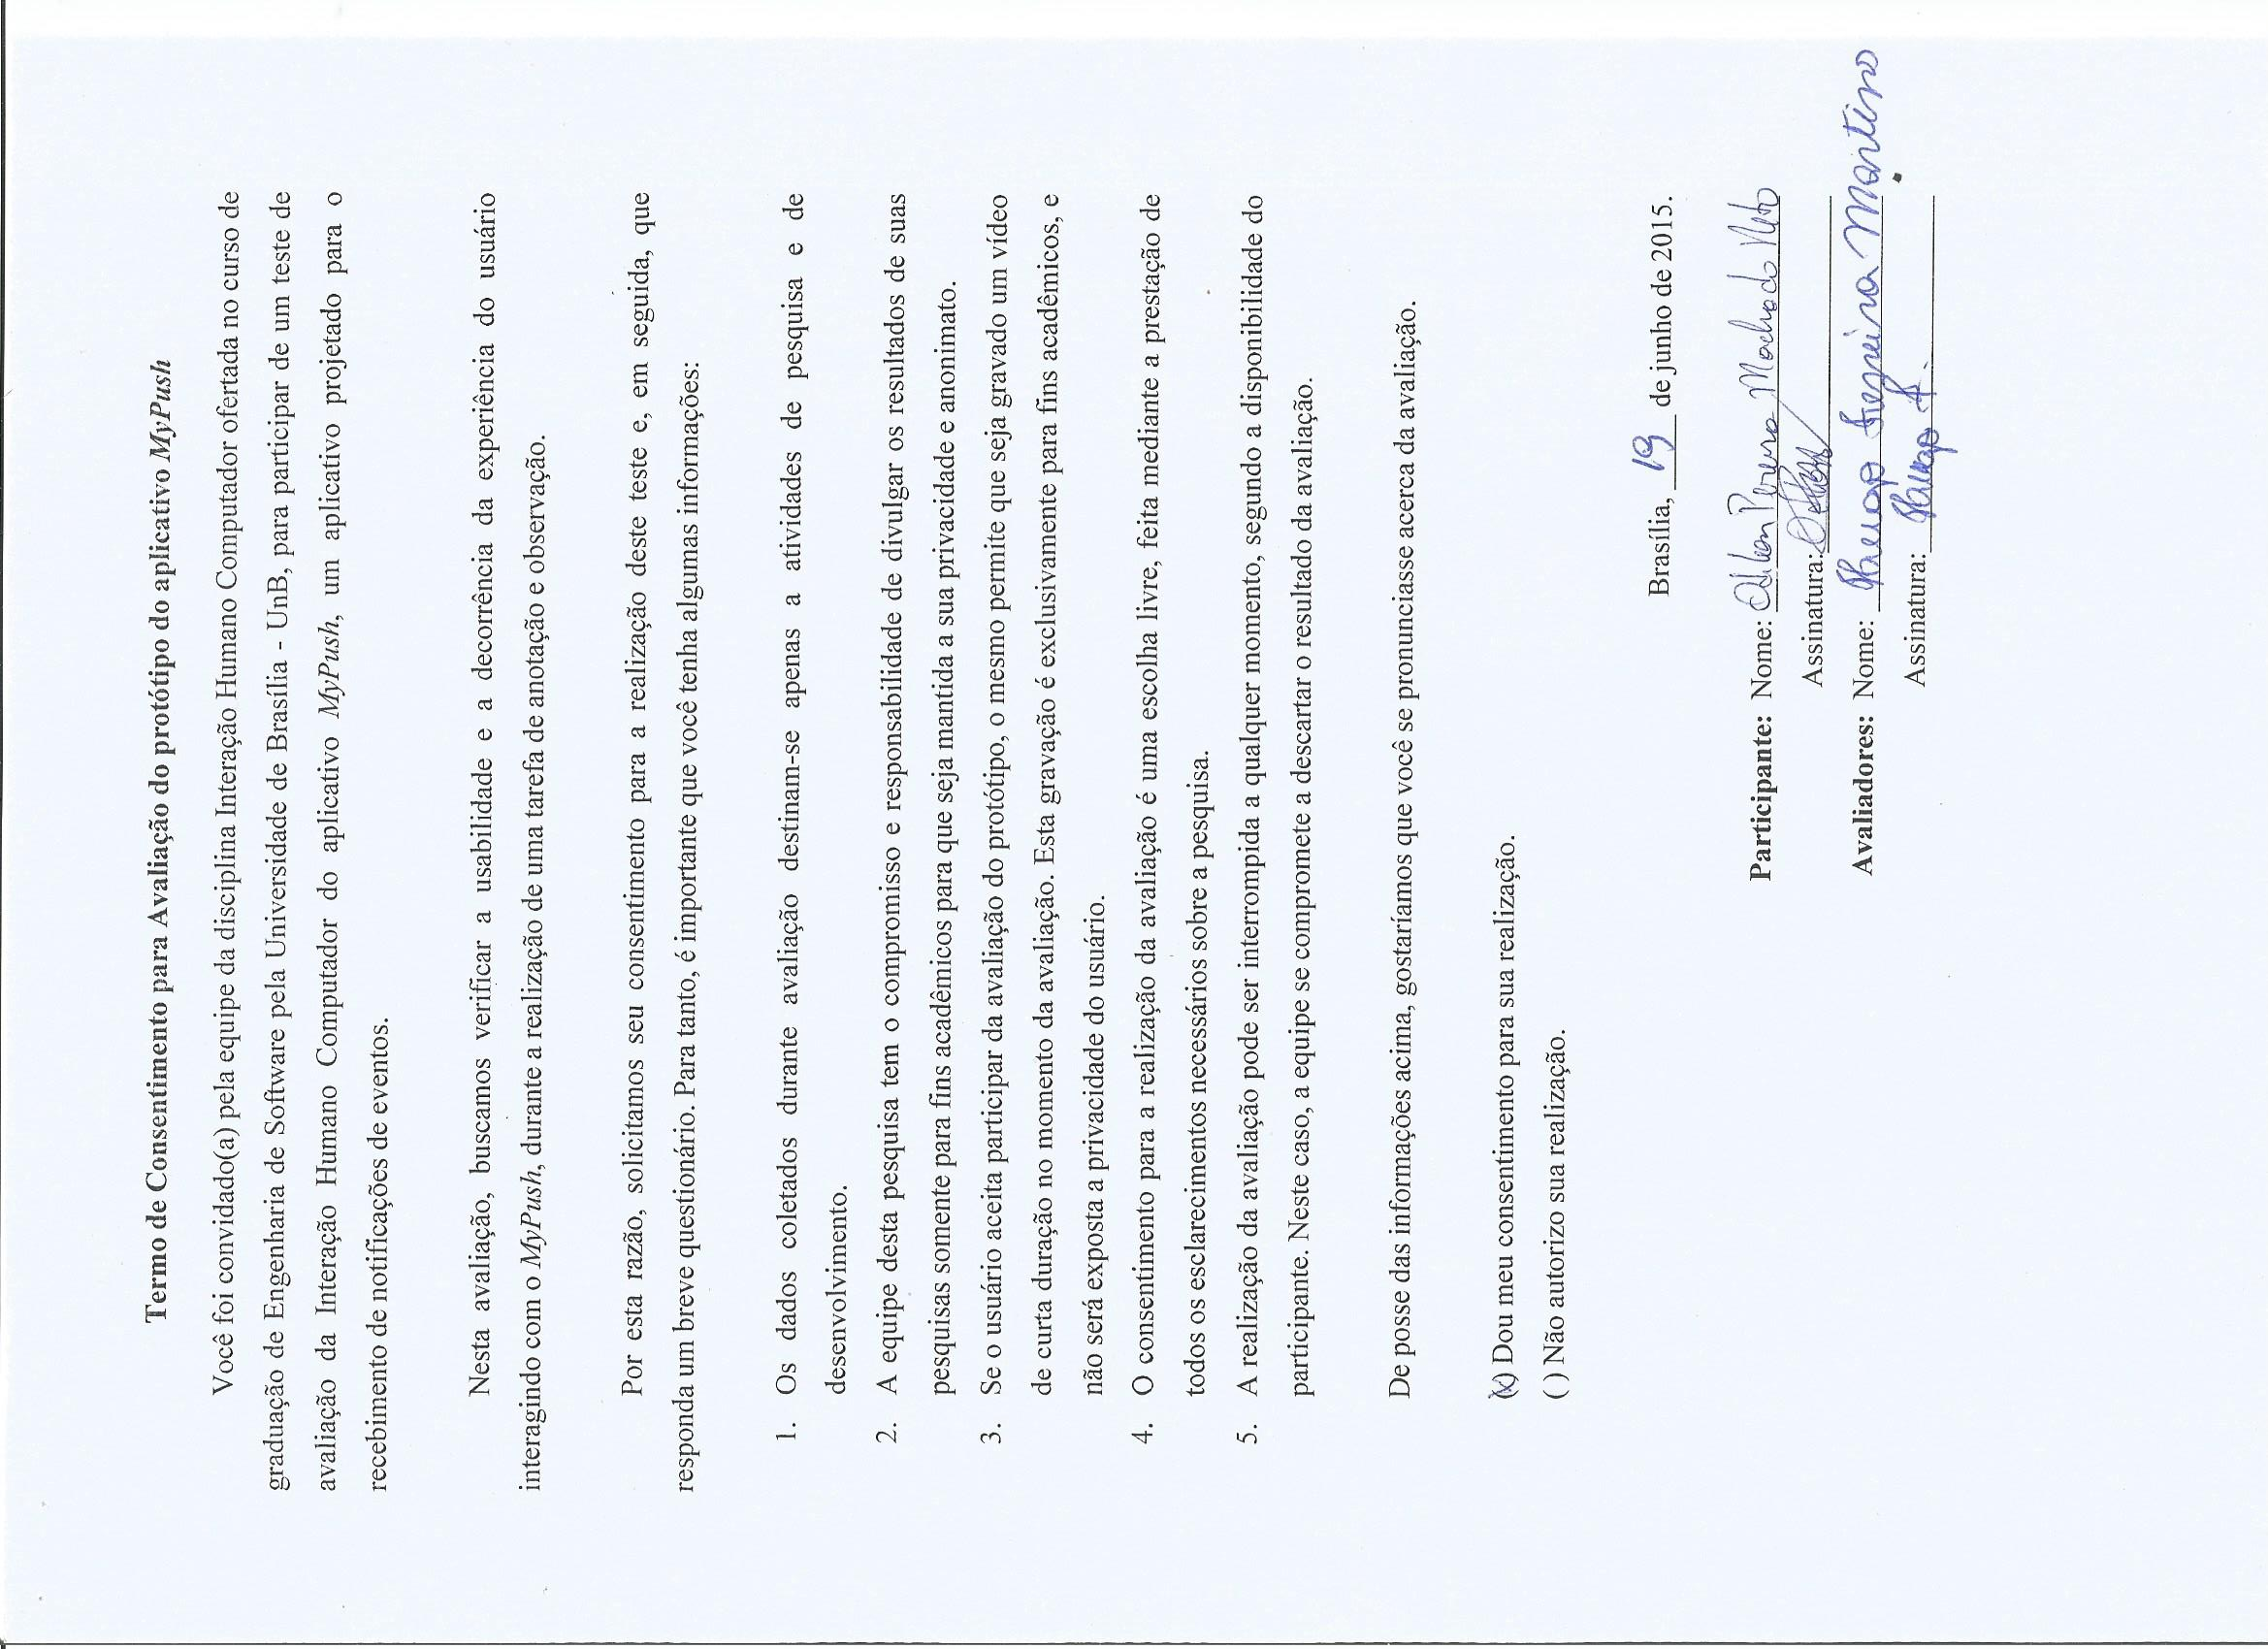
\includegraphics[scale=0.6, angle=-90]{editaveis/figuras/odilon}
      \caption{Termo de consentimento assinado por um dos usuários que participaram da avaliação.}
      \label{termo_consentimento_1}
    \end{figure}
    
    \section*{Usuário 18}
    \begin{figure}[!htbp]
      \centering
      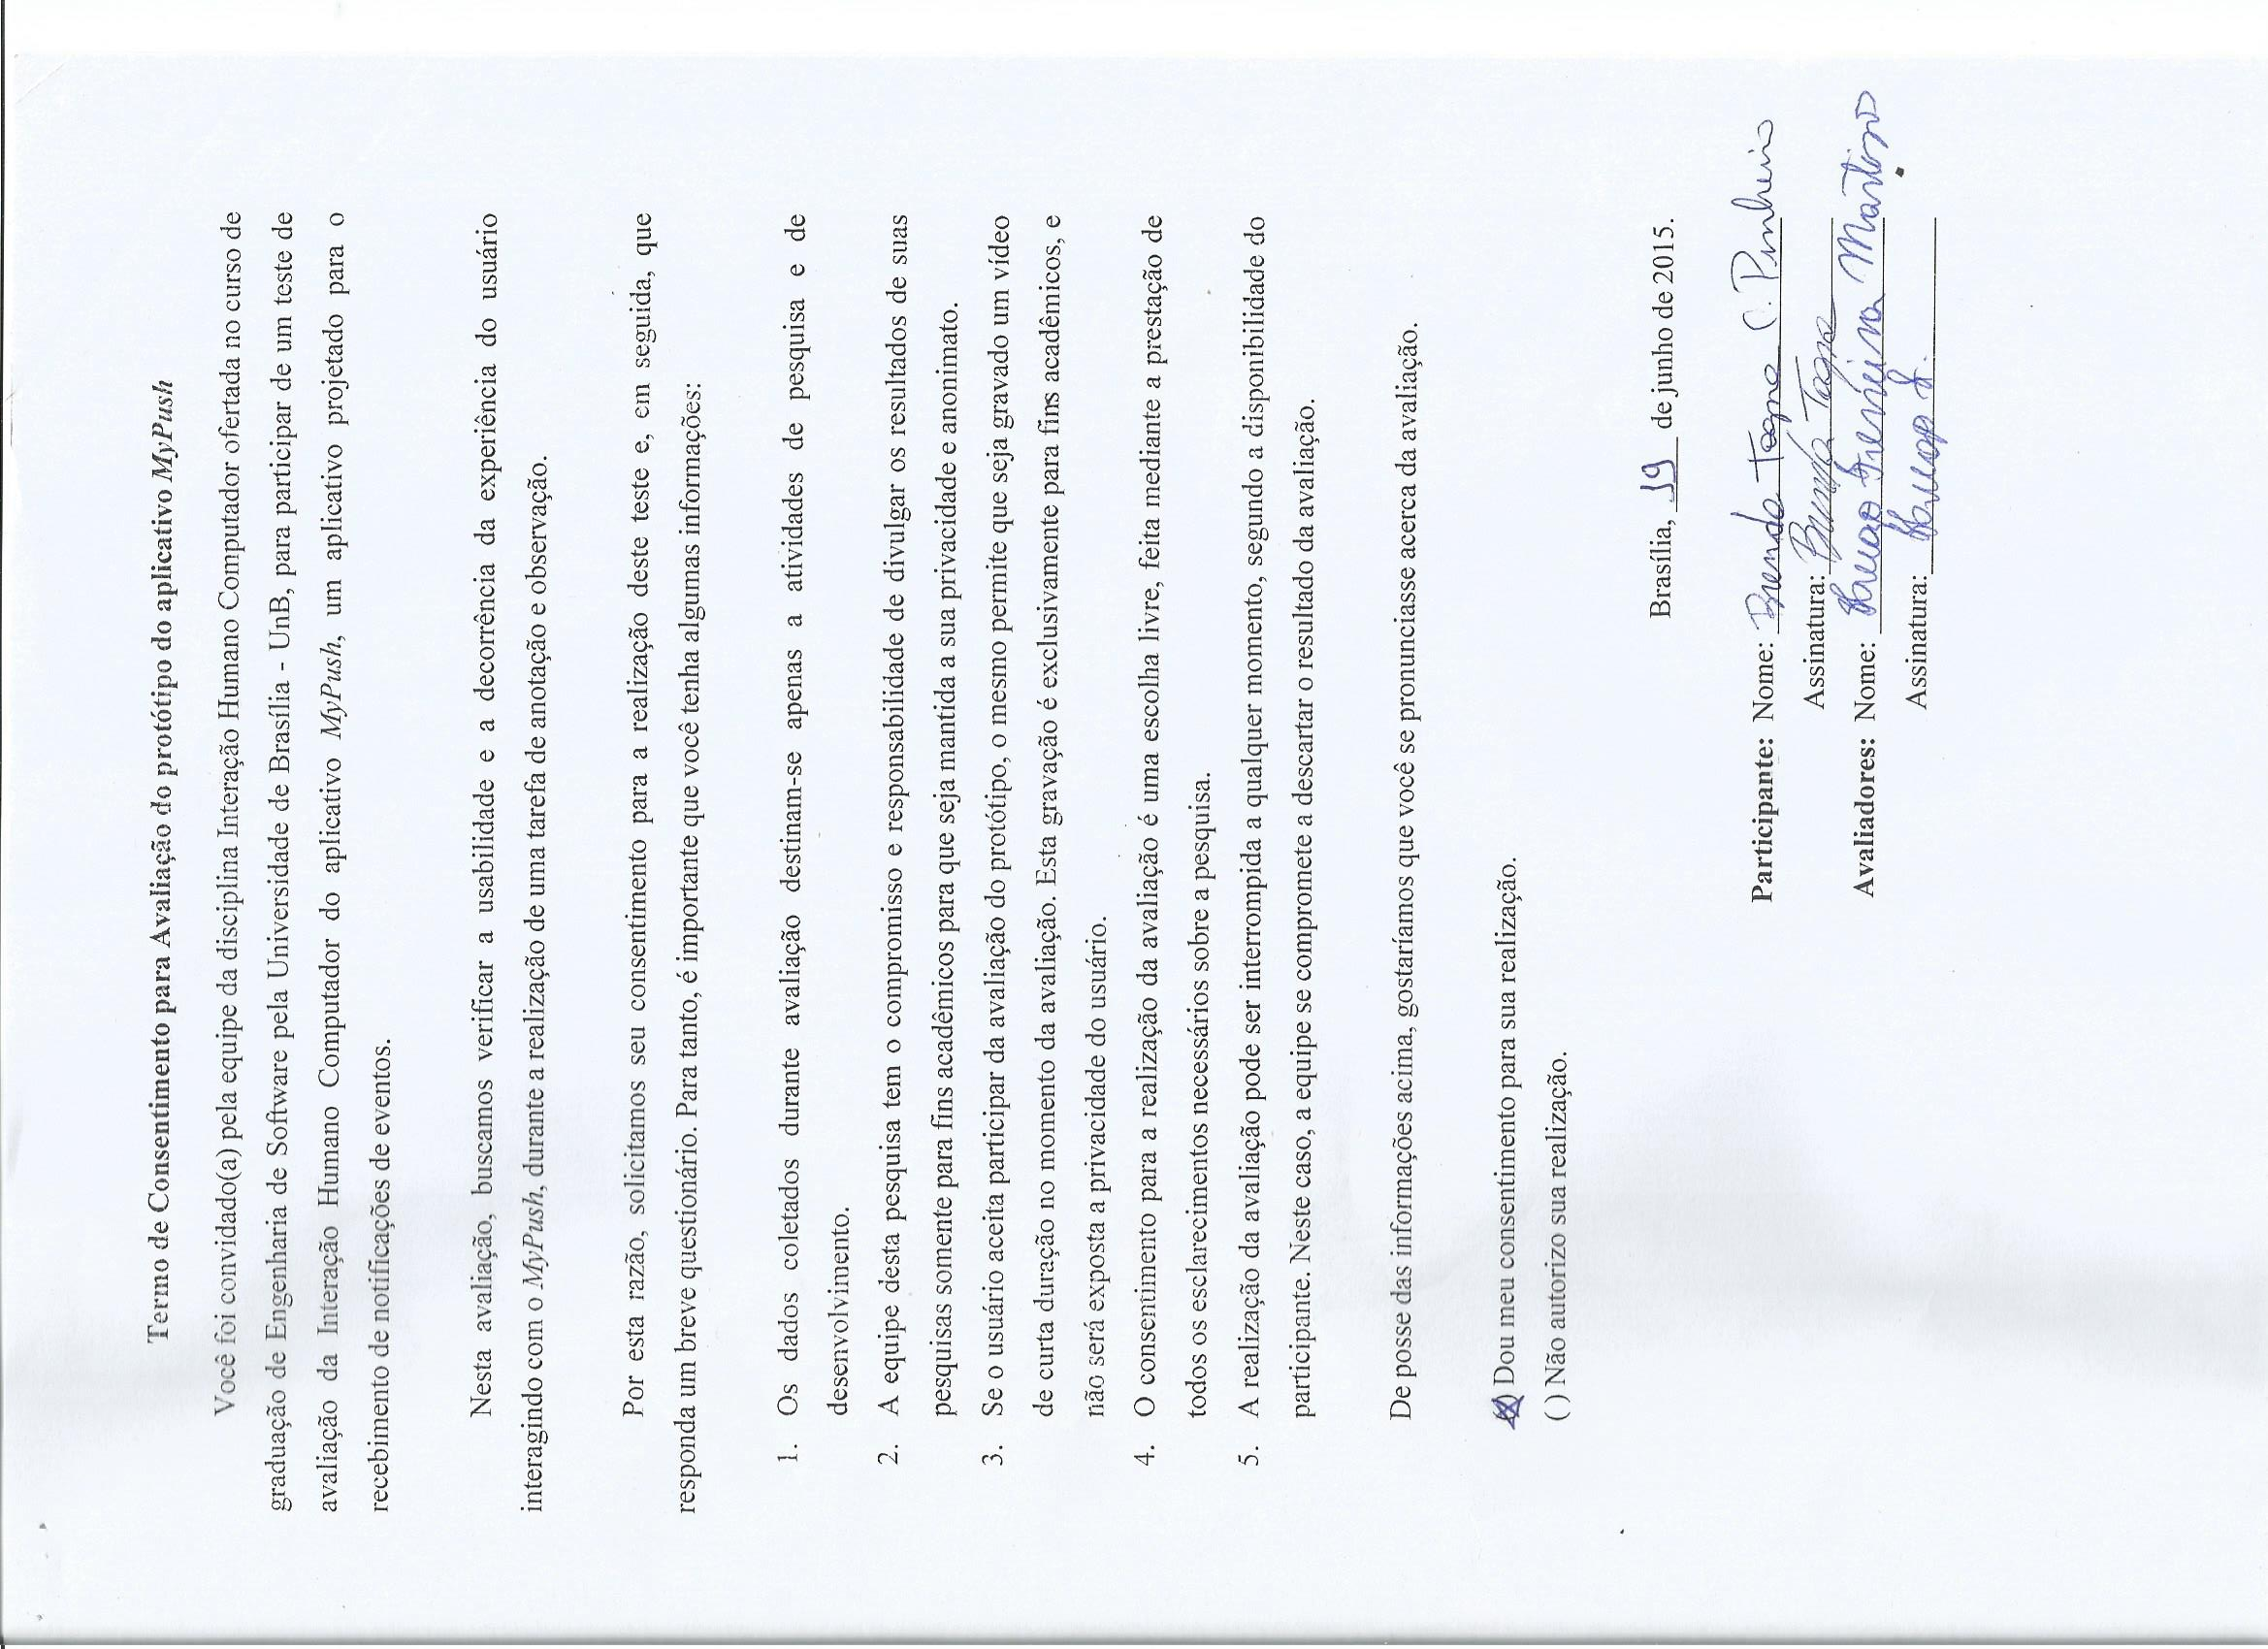
\includegraphics[scale=0.6, angle=-90]{editaveis/figuras/brenda}
      \caption{Termo de consentimento assinado por um dos usuários que participaram da avaliação.}
      \label{termo_consentimento_1}
    \end{figure}
    
    \section*{Usuário 19}
    \begin{figure}[!htbp]
      \centering
      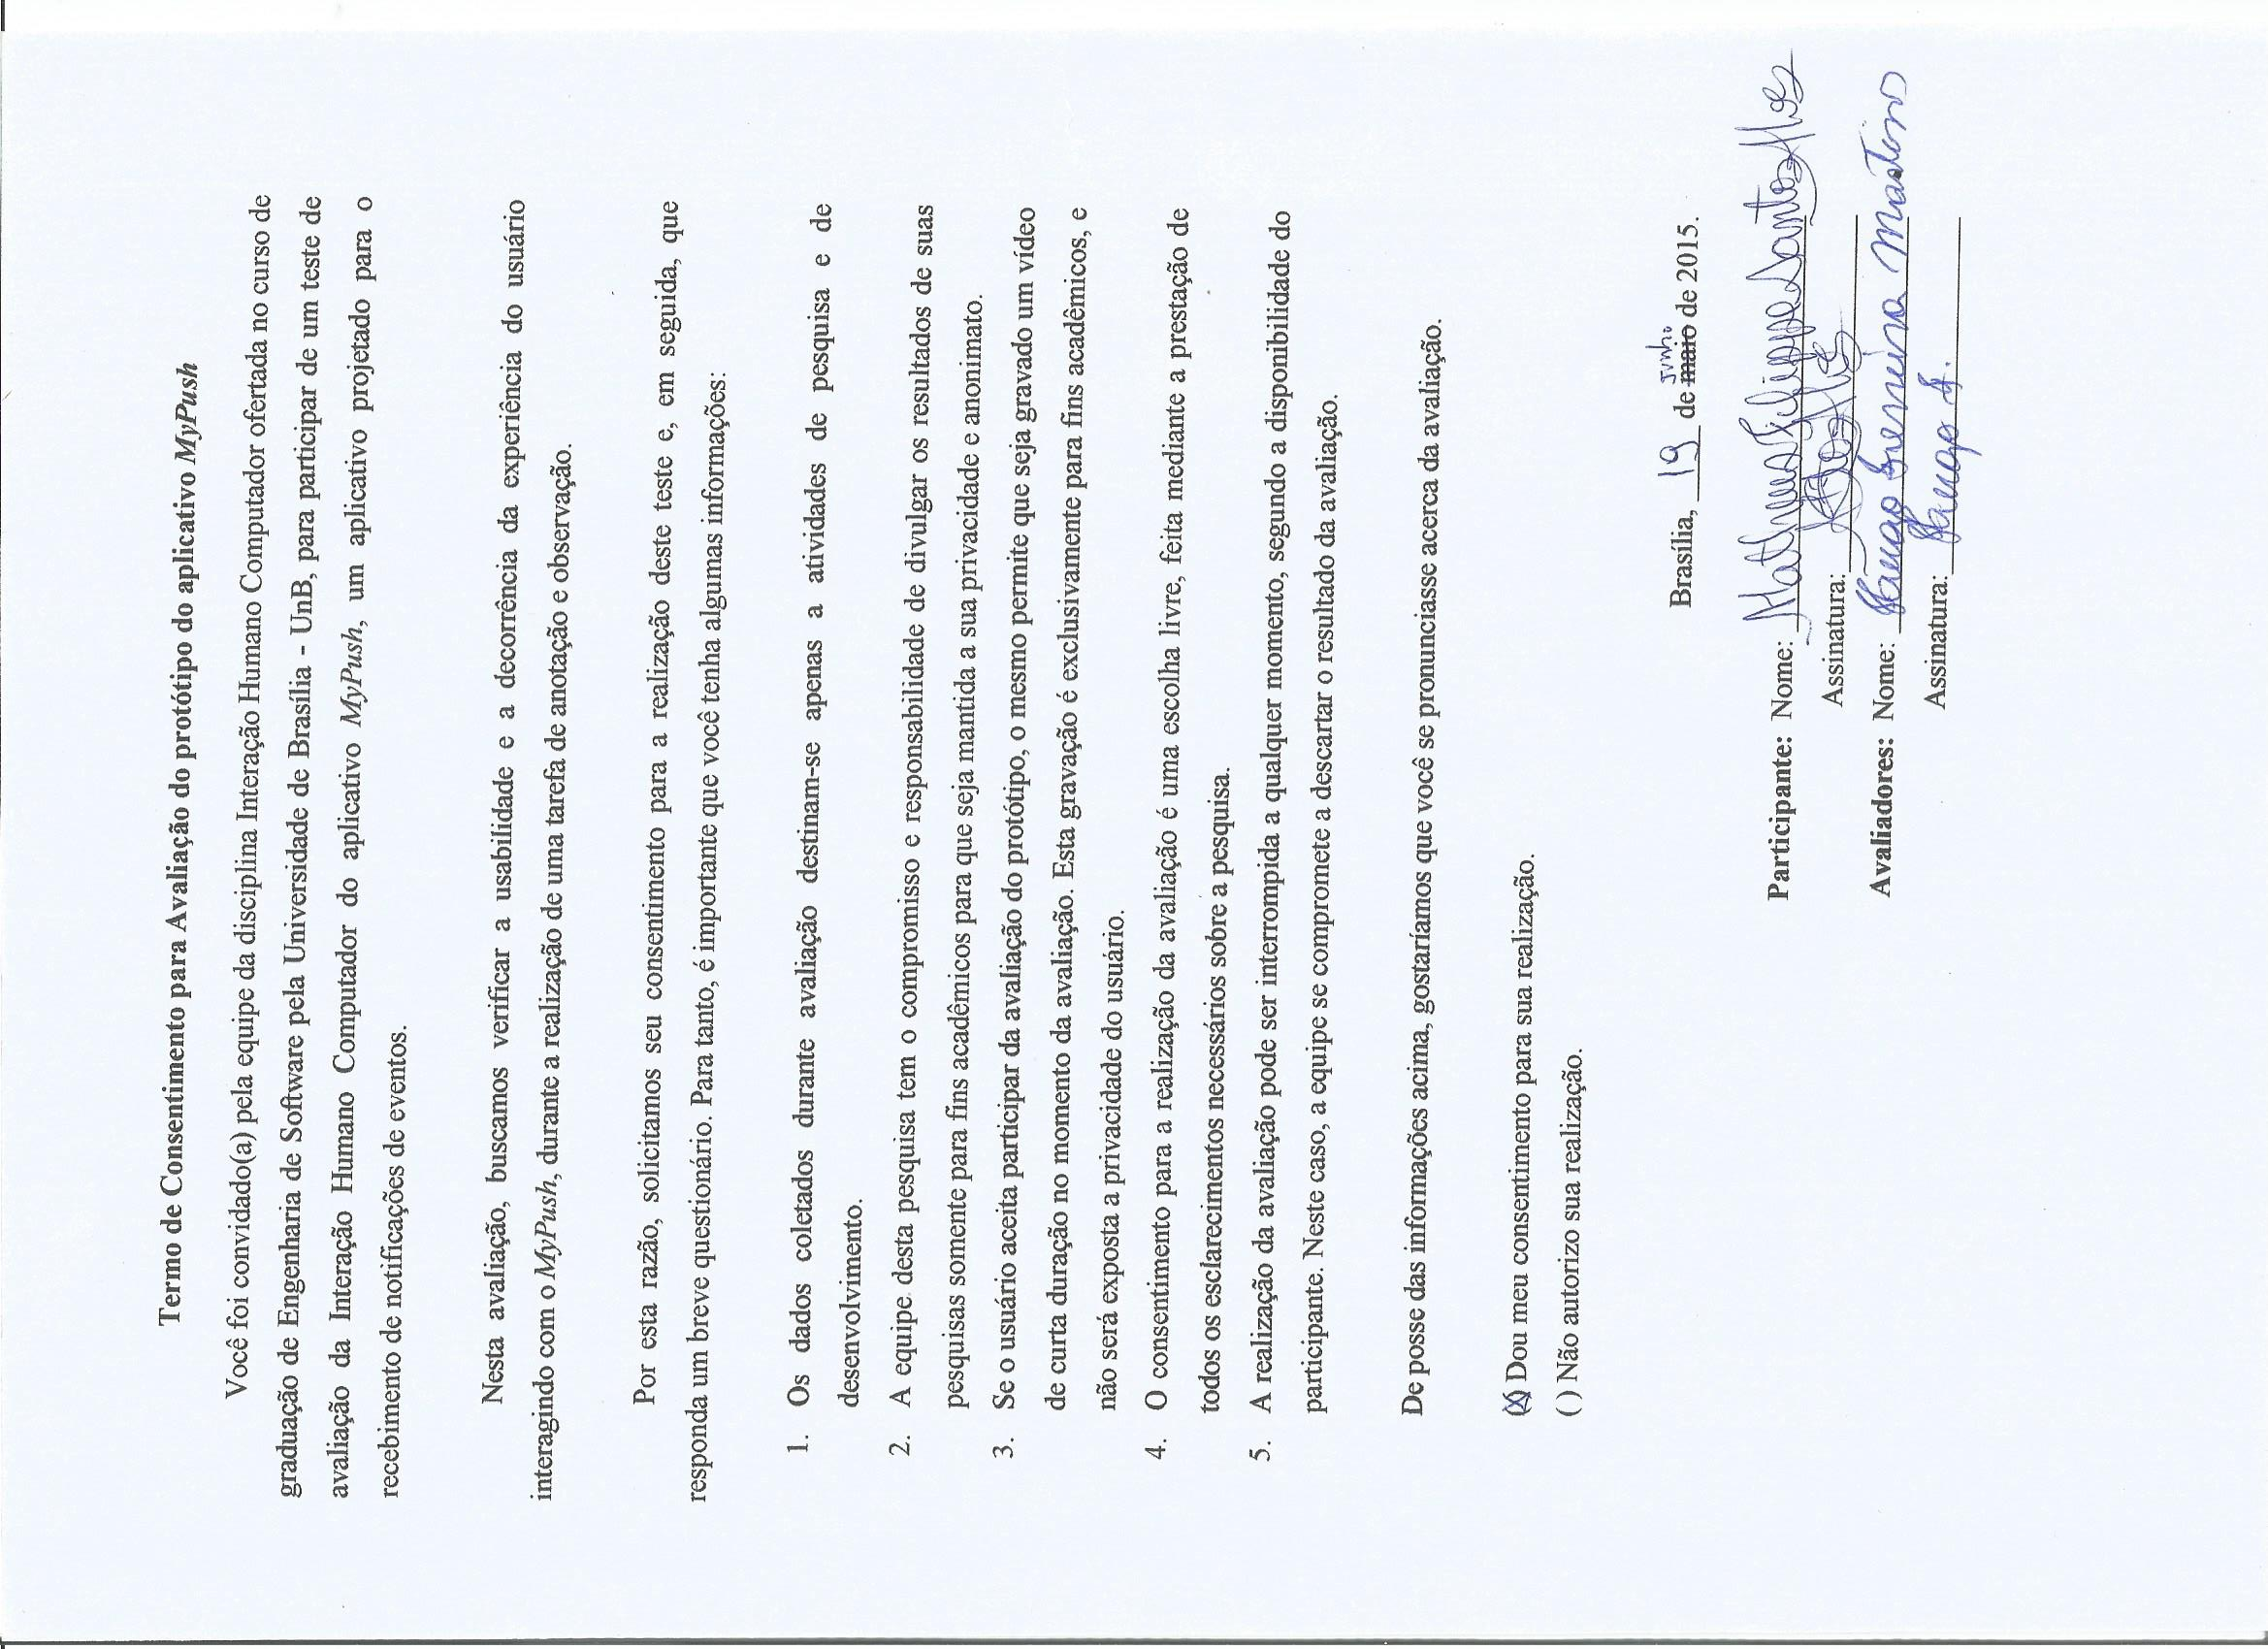
\includegraphics[scale=0.6, angle=-90]{editaveis/figuras/matheus_filippe}
      \caption{Termo de consentimento assinado por um dos usuários que participaram da avaliação.}
      \label{termo_consentimento_1}
    \end{figure}
    
    \section*{Usuário 20}
    \begin{figure}[!htbp]
      \centering
      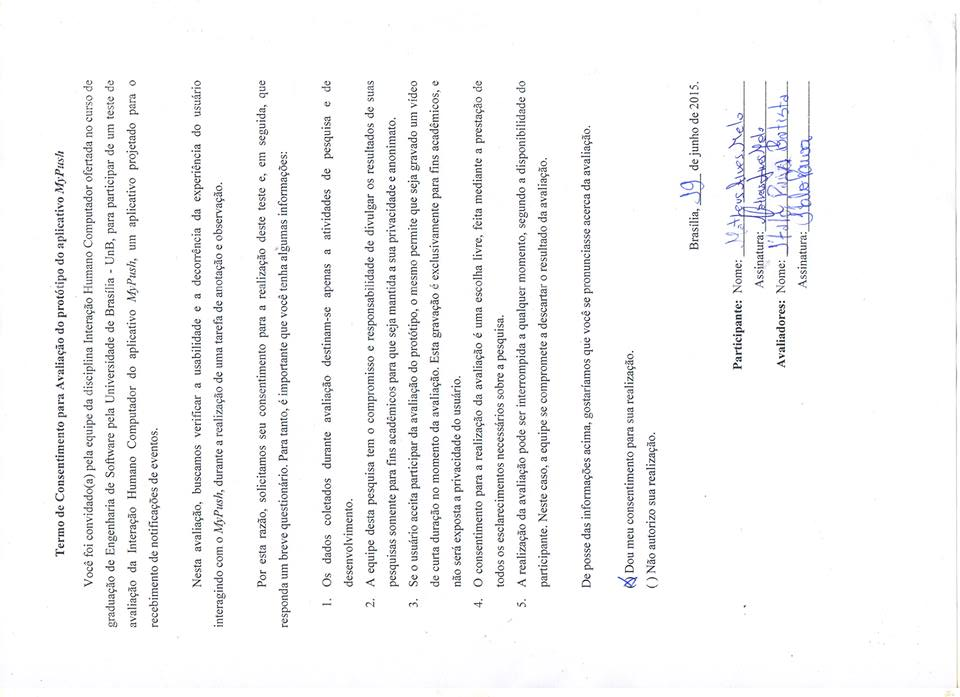
\includegraphics[scale=0.6, angle=-90]{editaveis/figuras/matheus_alves}
      \caption{Termo de consentimento assinado por um dos usuários que participaram da avaliação.}
      \label{termo_consentimento_1}
    \end{figure}
	
	
  \chapter{Questionário ASQ (traduzido)}
      
      O seguinte questionário foi proposto por Lewis (\citeyear{lewis91}) e traduzido para o português pelos autores.
      
      \section*{Itens}
	
	\begin{enumerate}
	  \item No geral, estou satisfeito com a facilidade de completar essa tarefa.
	  \item No geral, estou satisfeito com a quantidade de tempo que levou para completar essa tarefa.
	  \item No geral, estou satisfeito com as informações de suporte (ajudas online, mensagens, documentação)
	    oferecidas ao se completar essa tarefa.
	\end{enumerate}
      
      \section*{Padrão de resposta}
      
	O ASQ segue um padrão de resposta gradativo de sete escalas. Quanto mais perto de 1, mais o usuário concorda com a 
	afirmação feita no respectivo item, enquanto quanto mais perto de 7, mais o usuário discorda com a afirmação feita no
	respectivo item. Ainda é possível escolher a opção de "Não aplicável".\\
            
	\noindent
	\textbf{CONCORDO FORTEMENTE}   1    2    3    4    5    6    7    \textbf{DISCORDO FORTEMENTE}
	
  \chapter{Questionário PSSUQ (traduzido)}
    
    O seguinte questionário foi proposto por Lewis (\citeyear{lewis02}) e traduzido para o português pelos autores.
      
      \section*{Itens}
	
	\begin{enumerate}
	  \item No geral, estou satisfeito com o quão fácil foi de utilizar esse sistema.

	  \item Foi simples utilizar esse sistema.

	  \item Eu pude efetivamente completar as tarefas e cenários utilizando esse sistema.

	  \item Eu fui capaz de completar as tarefas e cenários rapidamente utilizando esse sistema.

	  \item Eu fui capaz de completar as tarefas e cenários utilizando esse sistema, eficientemente.

	  \item Me senti confortável utilizando esse sistema.

	  \item Foi fácil aprender a utilizar o sistema.

	  \item Acredito que poderia me tornar produtivo rapidamente utilizando esse sistema.

	  \item O sistema forneceu mensagens de erros que diziam claramente como consertar os problemas.

	  \item Quando eu cometia erros utilizando o sistema, era possível recuperar facil e rapidamente.

	  \item As informações de suporte fornecidas pelo sistema eram claras.

	  \item Foi fácil achar a informação que eu queria.

	  \item As informações fornecidas pelo sistema eram fáceis de serem compreendidas.

	  \item A informação foi efetiva em me ajudar a completar as tarefas e cenários.

	  \item A organização da informação na tela do sistema era clara.

	  \item A interface desse sistema é agradável.

	  \item Gostei de utilizar a interface desse sistema, era interessante.

	  \item O sistema possui todas as funcionalidades e capacidades que eu esperava.

	  \item No geral, estou satisfeito com esse sistema.
	\end{enumerate}
      
      \section*{Padrão de resposta}
      
	O PSSUQ também segue um padrão de resposta gradativo de sete escalas. Quanto mais perto de 1, mais o usuário concorda com a 
	afirmação feita no respectivo item, enquanto quanto mais perto de 7, mais o usuário discorda com a afirmação feita no
	respectivo item. Ainda é possível escolher a opção de "Não aplicável".\\
            
	\noindent
	\textbf{CONCORDO FORTEMENTE}   1    2    3    4    5    6    7    \textbf{DISCORDO FORTEMENTE}
    
  
\end{anexosenv}

